%======================================================================
% University of Waterloo Thesis Template for LaTeX 
% Last Updated August 2023
% by IST Client Services, 
% University of Waterloo, 200 University Ave. W., Waterloo, Ontario, Canada
% FOR ASSISTANCE, please send mail to ist-helpdesk@uwaterloo.ca

% DISCLAIMER
% To the best of our knowledge, this template satisfies the current uWaterloo thesis requirements.
% However, it is your responsibility to assure that you have met all requirements of the University and your particular department.

% Many thanks for the feedback from many graduates who assisted the development of this template.
% Also note that there are explanatory comments and tips throughout this template.
%======================================================================
% Some important notes on using this template and making it your own...

% The University of Waterloo has required electronic thesis submission since October 2006. 
% See the uWaterloo thesis regulations at
% https://uwaterloo.ca/graduate-studies/thesis.
% This thesis template is geared towards generating a PDF version optimized for viewing on an electronic display, including hyperlinks within the PDF.

% DON'T FORGET TO ADD YOUR OWN NAME AND TITLE in the "hyperref" package configuration below. 
% Search for: PDFTITLE, PDFAUTHOR, PDFSUBJECT, and PDFKEYWORDS.
% THIS INFORMATION GETS EMBEDDED IN THE FINAL PDF DOCUMENT.
% You can view the information if you view properties of the PDF document.

% Many faculties/departments also require one or more printed copies. 
% This template attempts to satisfy both types of output. 
% See additional notes below.
% It is based on the standard "book" document class which provides all necessary sectioning structures and allows multi-part theses.

% If you are using this template in Overleaf (cloud-based collaboration service), then it is automatically processed and previewed for you as you edit.

% For people who prefer to install their own LaTeX distributions on their own computers, and process the source files manually, the following notes provide the sequence of tasks:
 
% E.g. to process a thesis called "mythesis.tex" based on this template, run:

% pdflatex mythesis	-- first pass of the pdflatex processor
% bibtex mythesis	-- generates bibliography from .bib data file(s)
% makeindex         -- should be run only if an index is used 
% pdflatex mythesis	-- fixes numbering in cross-references, bibliographic references, glossaries, index, etc.
% pdflatex mythesis	-- it takes a couple of passes to completely process all cross-references

% If you use the recommended LaTeX editor, Texmaker, you would open the mythesis.tex file, then click the PDFLaTeX button. Then run BibTeX (under the Tools menu).
% Then click the PDFLaTeX button two more times. 
% If you have an index as well,you'll need to run MakeIndex from the Tools menu as well, before running pdflatex
% the last two times.

% N.B. The "pdftex" program allows graphics in the following formats to be included with the "\includegraphics" command: PNG, PDF, JPEG, TIFF
% Tip: Generate your figures and photos in the size you want them to appear in your thesis, rather than scaling them with \includegraphics options.
% Tip: Any drawings you do should be in scalable vector graphic formats: SVG, PNG, WMF, EPS and then converted to PNG or PDF, so they are scalable in the final PDF as well.
% Tip: Photographs should be cropped and compressed so as not to be too large.

% To create a PDF output that is optimized for double-sided printing: 
% 1) comment-out the \documentclass statement in the preamble below, and un-comment the second \documentclass line.
% 2) change the value assigned below to the boolean variable "PrintVersion" from " false" to "true".

%======================================================================
%   D O C U M E N T   P R E A M B L E
% Specify the document class, default style attributes, and page dimensions, etc.
% For hyperlinked PDF, suitable for viewing on a computer, use this:
\documentclass[letterpaper,12pt,titlepage,oneside,final]{book}
 
% For PDF, suitable for double-sided printing, change the PrintVersion variable below to "true" and use this \documentclass line instead of the one above:
%\documentclass[letterpaper,12pt,titlepage,openright,twoside,final]{book}

% Some LaTeX commands I define for my own nomenclature.
% If you have to, it's easier to make changes to nomenclature once here than in a million places throughout your thesis!
\newcommand{\package}[1]{\textbf{#1}} % package names in bold text
\newcommand{\cmmd}[1]{\textbackslash\texttt{#1}} % command name in tt font 
\newcommand{\href}[1]{#1} % does nothing, but defines the command so the print-optimized version will ignore \href tags (redefined by hyperref pkg).
%\newcommand{\texorpdfstring}[2]{#1} % does nothing, but defines the command
% Anything defined here may be redefined by packages added below...

%for margin altering per page
\usepackage{geometry}

% This package allows if-then-else control structures.
\usepackage{ifthen}
\newboolean{PrintVersion}
\setboolean{PrintVersion}{false}
% CHANGE THIS VALUE TO "true" as necessary, to improve printed results for hard copies by overriding some options of the hyperref package, called below.

%\usepackage{nomencl} % For a nomenclature (optional; available from ctan.org)
\usepackage{amsmath,amssymb,amstext} % Lots of math symbols and environments
% \usepackage{rotating}
\usepackage[pdftex]{graphicx} % For including graphics N.B. pdftex graphics driver 
\usepackage{float}
% Hyperlinks make it very easy to navigate an electronic document.
% In addition, this is where you should specify the thesis title and author as they appear in the properties of the PDF document.
% Use the "hyperref" package 
% N.B. HYPERREF MUST BE THE LAST PACKAGE LOADED; ADD ADDITIONAL PKGS ABOVE
\usepackage[pdftex,pagebackref=false]{hyperref} % with basic options
%\usepackage[pdftex,pagebackref=true]{hyperref}
		% N.B. pagebackref=true provides links back from the References to the body text. This can cause trouble for printing.
\hypersetup{
    plainpages=false,       % needed if Roman numbers in frontpages
    unicode=false,          % non-Latin characters in Acrobat’s bookmarks
    pdftoolbar=true,        % show Acrobat’s toolbar?
    pdfmenubar=true,        % show Acrobat’s menu?
    pdffitwindow=false,     % window fit to page when opened
    pdfstartview={FitH},    % fits the width of the page to the window
%    pdftitle={uWaterloo\ LaTeX\ Thesis\ Template},    % title: CHANGE THIS TEXT!
%    pdfauthor={Author},    % author: CHANGE THIS TEXT! and uncomment this line
%    pdfsubject={Subject},  % subject: CHANGE THIS TEXT! and uncomment this line
%    pdfkeywords={keyword1} {key2} {key3}, % list of keywords, and uncomment this line if desired
    pdfnewwindow=true,      % links in new window
    colorlinks=true,        % false: boxed links; true: colored links
    linkcolor=blue,         % color of internal links
    citecolor=green,        % color of links to bibliography
    filecolor=magenta,      % color of file links
    urlcolor=cyan           % color of external links
}
\ifthenelse{\boolean{PrintVersion}}{   % for improved print quality, change some hyperref options
\hypersetup{	% override some previously defined hyperref options
%    colorlinks,%
    citecolor=black,%
    filecolor=black,%
    linkcolor=black,%
    urlcolor=black}
}{} % end of ifthenelse (no else)

\usepackage[automake,toc,abbreviations]{glossaries-extra} % Exception to the rule of hyperref being the last add-on package
% If glossaries-extra is not in your LaTeX distribution, get it from CTAN (http://ctan.org/pkg/glossaries-extra), 
% although it's supposed to be in both the TeX Live and MikTeX distributions. There are also documentation and 
% installation instructions there.

% Setting up the page margins...
% uWaterloo thesis requirements specify a minimum of 1 inch (72pt) margin at the
% top, bottom, and outside page edges and a 1.125 in. (81pt) gutter margin (on binding side). 
% While this is not an issue for electronic viewing, a PDF may be printed, and so we have the same page layout for both printed and electronic versions, we leave the gutter margin in.
% Set margins to minimum permitted by uWaterloo thesis regulations:
\setlength{\marginparwidth}{0pt} % width of margin notes
% N.B. If margin notes are used, you must adjust \textwidth, \marginparwidth
% and \marginparsep so that the space left between the margin notes and page
% edge is less than 15 mm (0.6 in.)
\setlength{\marginparsep}{0pt} % width of space between body text and margin notes
\setlength{\evensidemargin}{0.125in} % Adds 1/8 in. to binding side of all 
% even-numbered pages when the "twoside" printing option is selected
\setlength{\oddsidemargin}{0.125in} % Adds 1/8 in. to the left of all pages when "oneside" printing is selected, and to the left of all odd-numbered pages when "twoside" printing is selected
\setlength{\textwidth}{6.375in} % assuming US letter paper (8.5 in. x 11 in.) and side margins as above
\raggedbottom

% The following statement specifies the amount of space between paragraphs. Other reasonable specifications are \bigskipamount and \smallskipamount.
\setlength{\parskip}{\medskipamount}

% The following statement controls the line spacing.  
% The default spacing corresponds to good typographic conventions and only slight changes (e.g., perhaps "1.2"), if any, should be made.
\renewcommand{\baselinestretch}{1} % this is the default line space setting

% By default, each chapter will start on a recto (right-hand side) page.
% We also force each section of the front pages to start on a recto page by inserting \cleardoublepage commands.
% In many cases, this will require that the verso (left-hand) page be blank, and while it should be counted, a page number should not be printed.
% The following statements ensure a page number is not printed on an otherwise blank verso page.
\let\origdoublepage\cleardoublepage
\newcommand{\clearemptydoublepage}{%
  \clearpage{\pagestyle{empty}\origdoublepage}}
\let\cleardoublepage\clearemptydoublepage

% Define Glossary terms (This is properly done here, in the preamble and could also be \input{} from a separate file...)
% Main glossary entries -- definitions of relevant terminology
\newglossaryentry{computer}
{
name=computer,
description={A programmable machine that receives input data,
               stores and manipulates the data, and provides
               formatted output}
}

% Nomenclature glossary entries -- New definitions, or unusual terminology
\newglossary*{nomenclature}{Nomenclature}
\newglossaryentry{dingledorf}
{
type=nomenclature,
name=dingledorf,
description={A person of supposed average intelligence who makes incredibly brainless misjudgments}
}

% List of Abbreviations (abbreviations type is built in to the glossaries-extra package)
% \newabbreviation{aaaaz}{AAAAZ}{American Association of Amateur Astronomers and Zoologists}

%\newabbreviation{nice}{NICE}{Newton direct and %Inverse Computation for Equilibrium}

\newglossaryentry{gpr}% the label
{%
  name={GPR},%
  description={Gaussian Process Regression is a method of performing inference on continuous values using a Gaussian process prior. A Gaussian process is a collection of random variables that have a joint multivariate normal distribution. A Gaussian process can be completely defined by its mean function and covariance function, which specify the expected value and the correlation of any finite subset of variables. Gaussian process regression uses the observed data to update the prior distribution and obtain a posterior distribution, which can be used to make predictions and estimate the uncertainty of the results.},
  % type={abbreviations},
  first={Gaussian Process Regression (GPR)},%
  text={GPR},%
  plural={GPR's}%
}

\newglossaryentry{mhd}% the label
{%
  name={MHD},%
  description={MHD stands for magnetohydrodynamics. It is a model of electrically conducting fluids that treats all interpenetrating particle species together as a single continuous medium. It is primarily concerned with the low-frequency, large-scale, magnetic behavior in plasmas and liquid metals.},
  % type={abbreviations},
  first={magnetohydrodynamics (MHD)},%
  text={MHD},%
}

\newglossaryentry{imas}% the label
{%
  name={IMAS},%
  description={ Integrated Modeling and Analysis Suite, is a framework and data management system. It is designed to store, manage, and analyze experimental and simulation data. IMAS provides a standardized platform for sharing and exchanging data among researchers from different institutions and countries. IMAS supports the integration of various fusion modeling codes and allows researchers to compare experimental data with simulation results.},
  % type={abbreviations},
  first={Integrated Modeling and Analysis Suite (IMAS)},%
  text={IMAS},%%
}


\newglossaryentry{sqp}% the label
{%
  name={SQP},%
  description={Sequential Quadratic Programming is a numerical optimization technique used to solve nonlinear constrained optimization problems. It is an iterative method that seeks to find the optimal solution to a problem by iteratively approximating it with a quadratic model and then solving this quadratic subproblem. The key idea is to successively update the solution in a way that moves closer to the optimal solution while satisfying the constraints.},%
  % type={abbreviations},
  first={Sequential Quadratic Programming (SQP)},%
  firstplural={Sequential Quadratic Programmings (SQPs)},%
  text={SQP},%
  plural={SQPs}%
}


\newglossaryentry{nice}% the label
{%
  name={NICE},%
  description={Newton direct and Inverse Computation for Equilibrium. A code developed by Blaise Faugeras at the Centre national de la recherche scientifique (CNRS) to numerically solve several plasma free-boundary equilibrium problems within a tokamak including the position of magnetic flux surfaces and the electron density profile.},%
  % type={abbreviations},
  first={Newton direct and Inverse Computation for Equilibrium (NICE)},%
  firstplural={Newton direct and Inverse Computation for Equilibriums (NICEs)},%
  text={NICE},%
  plural={NICE's}%
}

\newglossaryentry{west}% the label
{%
  name={WEST},%
  description={\textbf{Tungsten} (W) Environment in Steady-state Tokamak (WEST) is a French tokamak that aims to test and validate the ITER tungsten divertor components and prepare their safe operation},%
  % type={abbreviations},
  first={\textbf{Tungsten} (W) Environment in Steady-state Tokamak (WEST)},%
  text={WEST},%
  plural={WEST's}%
}

\newglossaryentry{mcmc}% the label
{%
  name={MCMC},%
  description={Markov chain Monte Carlo (MCMC) is a technique for sampling from complex and high-dimensional probability distributions that are difficult to sample from directly.},%
  % type={abbreviations},
  first={Markov chain Monte Carlo (MCMC)},%
  text={MCMC}%
}

\newglossaryentry{iat}% the label
{%
  name={IAT},%
  description={Integrated Autocorrelation Time (IAT) is a measure of how many steps it takes for a Markov chain to forget its initial state and become uncorrelated. It is defined as the sum of the normalized autocorrelations for all possible lags. It can be used to estimate the effective sample size and the Monte Carlo error of a chain.},%
  % type={abbreviations},
  first={Integrated Autocorrelation Time (IAT)},%
  text={IAT}%
}

\newglossaryentry{emcee}% the label
{%
  name={emcee},%
  description={emcee is a Python package that allows you to perform Markov chain Monte Carlo simulations using an ensemble of walkers that explore the parameter space in an affine-invariant way. This means that the shape of the posterior distribution does not affect the efficiency of the sampling.},%
  % type={abbreviations},
  % first={Integrated Autocorrelation Time (IAT)},%
  text={emcee}%
}
% List of Symbols
% \newglossary*{symbols}{List of Symbols}
% \newglossaryentry{rvec}
% {
% name={$\mathbf{v}$},
% sort={label},
% type=symbols,
% description={Random vector: a location in n-dimensional Cartesian space, where each dimensional component is determined by a random process}
% }

% \newglossaryentry{normr}
% {
% name={$\rho$},
% sort={label},
% type=symbols,
% description={Normalised Radius}
% }

% \newglossaryentry{sup}
% {
% name={$sup$},
% sort={label},
% type=symbols,
% description={wassap}
% }

% \newglossaryentry{biz}
% {
% name={$biz$},
% sort={label},
% type=symbols,
% description={biz}
% }
\makeglossaries

%======================================================================
%   L O G I C A L    D O C U M E N T
% The logical document contains the main content of your thesis.
% Being a large document, it is a good idea to divide your thesis into several files, each one containing one chapter or other significant chunk of content, so you can easily shuffle things around later if desired.
%======================================================================
\begin{document}

%----------------------------------------------------------------------
% FRONT MATERIAL
% title page, examining committee membership (for PhD Thesis only), declaration, borrowers' page, abstract, acknowledgements,
% dedication, table of contents, list of tables, list of figures, nomenclature, etc.
%----------------------------------------------------------------------
% T I T L E   P A G E
% -------------------
% Last updated August 24, 2023, by IST-Client Services
% The title page is counted as page `i' but we need to suppress the
% page number. Also, we don't want any headers or footers.
\pagestyle{empty}
\pagenumbering{roman}

% The contents of the title page are specified in the "titlepage"
% environment.
\begin{titlepage}
        \begin{center}
        \vspace*{-4.0cm}
        
\includegraphics[width = 400 px]{images/unilogos.png}

        % \HRule \\[0.4cm] % Horizontal line
        % {\huge \bfseries \ttitle}\\[0.4cm] % Thesis title
        % \HRule \\[1.5cm] % Horizontal line
        \vspace{1cm}
        \hrule % Horizontal line
        \vspace{0.3cm}
        {\Huge \bf Bayesian Inference of the 1D Electron Density Profile within the WEST Tokamak using Interferometry}
        \vspace{0.2cm}
        \hrule % Horizontal line
        
        \vspace*{1.0cm}

        \normalsize
        by \\

        \vspace*{1.0cm}

        \Large
        Daniel Jordan \\

        \vspace*{1.0cm}

        \normalsize
        A masters thesis presented to the University of Padova \\ 
        in fulfillment of the thesis requirement for the degree of \\
        Physics of Data \\

        \vspace*{1.0cm}

        \normalsize
        The research was carried out at Ghent University with onsite supervison from\\
        
        Geert Verdoolaege - Associate Professor\\
        Hao Wu - PhD Student\\
        \vspace{0.5cm}
        Remote supervision from the university of Padova was provided by\\
        
        Lidia Piron - Assistant Professor
        

        \vspace*{2.0cm}

        2023 \\
        \end{center}
\end{titlepage}


% The rest of the front pages should contain no headers and be numbered using Roman numerals starting with `ii'
\pagestyle{plain}
\setcounter{page}{2}

\cleardoublepage % Ends the current page and causes all figures and tables that have so far appeared in the input to be printed.
% In a two-sided printing style, it also makes the next page a right-hand (odd-numbered) page, producing a blank page if necessary.
\phantomsection    % allows hyperref to link to the correct page

% D E C L A R A T I O N   P A G E
% -------------------------------
  % The following is a sample Declaration Page as provided by the GSPA
  % December 13th, 2006.  It is designed for an electronic thesis.
 \addcontentsline{toc}{chapter}{Author's Declaration}
 \begin{center}\textbf{Author's Declaration}\end{center}

 % Author's Declaration Option ONE - line 118:  
 \noindent
I hereby declare that I am the sole author of this thesis. This is a true copy of the thesis, including any required final revisions, as accepted by my examiners.
  % Author's Declaration Option TWO - line 121. Updated August 21st, 2023. Use the following declaration text if appropriate by removing the percent character and space at the beginning of line 121, and add a percent symbol and space at line 118 to change Author's Declaration Option ONE to a remark that is not printed.
 \noindent  
% This thesis consists of material all of which I authored or co-authored: see Statement of Contributions included in the thesis. This is a true copy of the thesis, including any required final revisions, as accepted by my examiners.
  \bigskip
  
  \noindent
I understand that my thesis may be made electronically available to the public.

\cleardoublepage
\phantomsection    % allows hyperref to link to the correct page

% A B S T R A C T
% ---------------
\addcontentsline{toc}{chapter}{Abstract}
\begin{center}\textbf{Abstract}\end{center}

The abstract should briefly highlight the importance of the research and present its key findings. 

The electron density profile is a key parameter that affects the performance and stability of tokamak plasmas. 

\cleardoublepage
\phantomsection    % allows hyperref to link to the correct page

% A C K N O W L E D G E M E N T S
% -------------------------------
\addcontentsline{toc}{chapter}{Acknowledgements}
\begin{center}\textbf{Acknowledgements}\end{center}

A big thank you to Hao Wu, Jeffrey de Rycke, and Yangyang Zhang for their enlightening conversation and mentorship. I thank the rest of the team at infusion UGent, Geert Verdoolaege, Sven Van Loo, Jerome Alhage, Leonardo Caputo, and Joseph Hall for accepting me into their research group and including me in their research discussions. An extra thank you to Geert Verdoolaege for giving me this enriching opportunity.
\cleardoublepage
\phantomsection    % allows hyperref to link to the correct page

% D E D I C A T I O N
% -------------------
% \addcontentsline{toc}{chapter}{Dedication}
% \begin{center}\textbf{Dedication}\end{center}

% This is dedicated to the one I love.
% \cleardoublepage
% \phantomsection    % allows hyperref to link to the correct page

% T A B L E   O F   C O N T E N T S
% ---------------------------------
\renewcommand\contentsname{Table of Contents}
\tableofcontents
\cleardoublepage
\phantomsection    % allows hyperref to link to the correct page

% L I S T   O F   F I G U R E S
% -----------------------------
\addcontentsline{toc}{chapter}{List of Figures}
\listoffigures
\cleardoublepage
\phantomsection		% allows hyperref to link to the correct page

% L I S T   O F   T A B L E S
% ---------------------------
% \addcontentsline{toc}{chapter}{List of Tables}
% \listoftables
% \cleardoublepage
% \phantomsection		% allows hyperref to link to the correct page

% L I S T   O F   A B B R E V I A T I O N S
% ---------------------------
% \renewcommand*{\abbreviationsname}{List of Abbreviations}
% \printglossary[type=abbreviations]
% \cleardoublepage
% \phantomsection		% allows hyperref to link to the correct page

% L I S T   O F   S Y M B O L S
% ---------------------------
% \printglossary[type=symbols]
% \cleardoublepage
% \phantomsection		% allows hyperref to link to the correct page


% Change page numbering back to Arabic numerals
\pagenumbering{arabic}

 

%----------------------------------------------------------------------
% MAIN BODY
% We suggest using a separate file for each chapter of your thesis.
% Start each chapter file with the \chapter command.
% Only use \documentclass or \begin{document} and \end{document} commands in this master document.
% Tip: Putting each sentence on a new line is a way to simplify later editing.
%----------------------------------------------------------------------
% %======================================================================
\chapter{Introduction}
%======================================================================
In the beginning, there was $\pi$:

\begin{equation}
   e^{\pi i} + 1 = 0  \label{eqn_pi}
\end{equation}
A \gls{computer} could compute $\pi$ all day long. In fact, subsets of digits of $\pi$'s decimal approximation would make a good source for psuedo-random vectors, \gls{rvec} 

also \gls{normr}. 

%----------------------------------------------------------------------
\section{State of the Art}
%----------------------------------------------------------------------

See equation \ref{eqn_pi} on page \pageref{eqn_pi}.\footnote{A famous equation.}

\section{Some Meaningless Stuff}

The credo of the \gls{aaaaz} was, for several years, several paragraphs of gibberish, until the \gls{dingledorf} responsible for the \gls{aaaaz} Web site realized his mistake:

"Velit dolor illum facilisis zzril ipsum, augue odio, accumsan ea augue molestie lobortis zzril laoreet ex ad, adipiscing nulla. Veniam dolore, vel te in dolor te, feugait dolore ex vel erat duis nostrud diam commodo ad eu in consequat esse in ut wisi. Consectetuer dolore feugiat wisi eum dignissim tincidunt vel, nostrud, at vulputate eum euismod, diam minim eros consequat lorem aliquam et ad. Feugait illum sit suscipit ut, tation in dolore euismod et iusto nulla amet wisi odio quis nisl feugiat adipiscing luptatum minim nisl, quis, erat, dolore. Elit quis sit dolor veniam blandit ullamcorper ex, vero nonummy, duis exerci delenit ullamcorper at feugiat ullamcorper, ullamcorper elit vulputate iusto esse luptatum duis autem. Nulla nulla qui, te praesent et at nisl ut in consequat blandit vel augue ut.

Illum suscipit delenit commodo augue exerci magna veniam hendrerit dignissim duis ut feugait amet dolor dolor suscipit iriure veniam. Vel quis enim vulputate nulla facilisis volutpat vel in, suscipit facilisis dolore ut veniam, duis facilisi wisi nulla aliquip vero praesent nibh molestie consectetuer nulla. Wisi nibh exerci hendrerit consequat, nostrud lobortis ut praesent dignissim tincidunt enim eum accumsan. Lorem, nonummy duis iriure autem feugait praesent, duis, accumsan tation enim facilisi qui te dolore magna velit, iusto esse eu, zzril. Feugiat enim zzril, te vel illum, lobortis ut tation, elit luptatum ipsum, aliquam dolor sed. Ex consectetuer aliquip in, tation delenit dignissim accumsan consequat, vero, et ad eu velit ut duis ea ea odio.

Vero qui, te praesent et at nisl ut in consequat blandit vel augue ut dolor illum facilisis zzril ipsum. Exerci odio, accumsan ea augue molestie lobortis zzril laoreet ex ad, adipiscing nulla, et dolore, vel te in dolor te, feugait dolore ex vel erat duis. Ut diam commodo ad eu in consequat esse in ut wisi aliquip dolore feugiat wisi eum dignissim tincidunt vel, nostrud. Ut vulputate eum euismod, diam minim eros consequat lorem aliquam et ad luptatum illum sit suscipit ut, tation in dolore euismod et iusto nulla. Iusto wisi odio quis nisl feugiat adipiscing luptatum minim. Illum, quis, erat, dolore qui quis sit dolor veniam blandit ullamcorper ex, vero nonummy, duis exerci delenit ullamcorper at feugiat. Et, ullamcorper elit vulputate iusto esse luptatum duis autem esse nulla qui.

Praesent dolore et, delenit, laoreet dolore sed eros hendrerit consequat lobortis. Dolor nulla suscipit delenit commodo augue exerci magna veniam hendrerit dignissim duis ut feugait amet. Ad dolor suscipit iriure veniam blandit quis enim vulputate nulla facilisis volutpat vel in. Erat facilisis dolore ut veniam, duis facilisi wisi nulla aliquip vero praesent nibh molestie consectetuer nulla, iriure nibh exerci hendrerit. Vel, nostrud lobortis ut praesent dignissim tincidunt enim eum accumsan ea, nonummy duis. Ad autem feugait praesent, duis, accumsan tation enim facilisi qui te dolore magna velit, iusto esse eu, zzril vel enim zzril, te. Nisl illum, lobortis ut tation, elit luptatum ipsum, aliquam dolor sed minim consectetuer aliquip.

Tation exerci delenit ullamcorper at feugiat ullamcorper, ullamcorper elit vulputate iusto esse luptatum duis autem esse nulla qui. Volutpat praesent et at nisl ut in consequat blandit vel augue ut dolor illum facilisis zzril ipsum, augue odio, accumsan ea augue molestie lobortis zzril laoreet. Ex duis, te velit illum odio, nisl qui consequat aliquip qui blandit hendrerit. Ea dolor nonummy ullamcorper nulla lorem tation laoreet in ea, ullamcorper vel consequat zzril delenit quis dignissim, vulputate tincidunt ut."
%======================================================================
\chapter{Introduction}
%======================================================================
Nuclear fusion, the process by which two light atomic nuclei combine to form a heavier nucleus, holds the promise of revolutionizing the world's energy landscape. With the ever-increasing demand for sustainable, clean, and virtually limitless energy sources, nuclear fusion has emerged as a leading candidate. Nuclear fusion, in contrast to the fission processes used in current nuclear power plants, presents a fundamentally safer and more sustainable option. The primary fuel for fusion, isotopes of hydrogen, is abundant and can be extracted from water sources. Fusion reactions produce no long-lived, highly radioactive waste, minimizing environmental hazards and long-term disposal issues. Recent advancements have reignited interest in the field, with notable breakthroughs such as the development of high-temperature superconducting magnets, which enable the efficient confinement of high-energy plasma. An excelent example is the rare earth barium copper oxide high-temperature superconducting magnets that are being deployed in the SPARC experimental reactor \cite{SPARCoverview}. In February 2022, the UK-based JET laboratory reported that it had smashed its own world record for the amount of energy it could extract by squeezing together two forms of hydrogen, deuterium and tritium. The experiments produced 59 megajoules of energy over five seconds (11 megawatts of power), which was more than double what was achieved in similar tests back in 1997. Another breakthrough was announced in December 2022 by US scientists at the National Ignition Facility in California. They confirmed that they had achieved ignition for the first time, by firing up to 192 giant lasers into a peppercorn-sized fuel pellet and triggering a fusion reaction that released more energy than was put in by the lasers \cite{nationalignitionfacilitycali}.

Tokamaks are a class of fusion device with a great potential to achieve commercial fusion energy production. Tokamaks use magnetic fields to confine and heat plasma, a state of matter where atoms are split into electrons and nuclei. The immence pressures and temperatures created induce fusion reactions between light nuclei, such as hydrogen, to produce energy. Tokamaks currently demonste long plasma confinement times, which measure how well the plasma is isolated from the surrounding environment and affect the efficiency of energy production and heat loss. Tokamaks have the most extensive scientific and technological knowledge base, which has been accumulated over decades of research and development. This leads to reliable and robust designs, advanced diagnostics and control systems, and proven solutions for engineering challenges. These advantages make tokamaks the most promising candidates for achieving commercial fusion energy in the near future. Tokamaks have already shown impressive results in terms of fusion power output and energy gain. They are expected to reach even higher levels of performance with the next generation of devices. Tokamaks are also supported by a strong international collaboration and a clear roadmap for development. Therefore, tokamaks have a huge potential to commercialise fusion before other methods: especially with ITER just around the corner and plans for DEMO already underway. ITER and DEMO are complementary projects that will advance fusion energy from the experimental stage to the commercial stage. ITER will provide the scientific and technological basis for DEMO, which will be the first fusion power plant to produce electricity and operate with a closed fuel cycle. The construction of ITER is expected to be completed by 2025, and the first plasma operation is planned for 2026. The full deuterium-tritium operation of ITER is scheduled for 2035, which will coincide with the start of the construction of DEMO. The operation of DEMO is foreseen to begin in the 2040s, and to demonstrate the viability of fusion energy for commercial use.

The electron density profile is a key parameter that affects the performance and stability of tokamak plasmas. It affects the plasma current, the confinement time, the energy transport, the magnetohydrodynamic (MHD) modes, and the coupling of external heating and current drive sources. There are physical limits that constrain the maximum achievable density in tokamak plasmas. One of the most well-known density limits is the Greenwald limit, which states that the line-averaged density cannot exceed a value proportional to the plasma current divided by the plasma cross-sectional area. This limit is empirically observed in many tokamaks, and attempts to exceed it result in disruptions or edge localized modes (ELMs). The physical mechanism behind the Greenwald limit is not fully understood, but it may be related to the stability of the edge pedestal, the bootstrap current, or the core particle transport. A lower electron density leads to runaway electrons. The magnetic fields accelerate the electrons continously and only colisions prevent them from gaining enough energy to escape the magnetic confinement. A low density can mean that collisions are not frequent enough to prevent escape and the electrons can cause serious damage to the plasma facing wall. Thus it is not benificial for the plasmas electron density profile to be such as to have many electrons with a low density near the edge. 

One of the main challenges in measuring the electron density profile is to obtain high spatial and temporal resolution over a wide radial range. Several diagnostic techniques have been developed and applied to tokamaks, such as interferometry, reflectometry, Thomson scattering, and spectroscopy. Each technique has its own advantages and limitations in terms of accuracy, reliability, coverage, and invasiveness. A combination of different techniques is often used to obtain a comprehensive picture of the electron density profile evolution.

Another worthy challenge is to maintain the electron density profile in a desired shape. The electron density profile is influenced by various factors, such as plasma geometry/magnetic configuration, plasma current and pressure, impurity content, fueling and pumping methods, and external heating and current drive sources. Some of these factors can be manipulated by the operators, others can be controlled in real time with sophisticated algorythems and feedback loops; achieving a favorable electron density profile that enhances the plasma performance and stability.

The electron density profile is an important parameter that determines many aspects of tokamak plasmas. Measuring and controlling the electron density profile is a crucial task for optimizing the tokamak operation and achieving fusion energy goals.

This thesis focuses on performing a Bayesian inference of the electron density profile using the interferometry diagnostic and a Gaussian process prior. Bayesian inference with a Gaussian process prior is a powerful technique for nonparametric modeling of complex and nonlinear phenomena. A Gaussian process is a collection of random variables, of which have a joint Gaussian distribution. A Gaussian process can be specified by a mean vector and a covariance matrix, which encode the prior assumptions about the unknown profile to be learned. By applying Bayes’ rule, one can obtain the posterior distribution of the profile given some observed data, and use it for prediction and uncertainty quantification. Interferometry is a technique that uses the interference of electromagnetic waves to measure the properties of a medium. An interferometer consists of a coherent source of radiation, such as a laser, that is split into two beams: one that passes through the plasma and one that bypasses it. The two beams are then recombined and detected by a receiver. The phase difference between the two beams depends on the difference in the optical path length, which is affected by the electron density along the line of sight. By measuring the phase difference, one can calculate the line-averaged electron density of the plasma. The interferometer within a tokamk consists of many such laser beams penetrating the plasma at various angles. This thesis uses the \gls{west} tokmak's laser geometry which covers a span of the polodial cross section. Although there is not enough information to completly and accuratly reconstruct the electron density profile a best guess given the data can be infered. It is difficult or impossible to know how close any inffered profile is to the true profile.

Bayesian integrated analysis is often used to combine multiple diagnostics which measure the same or related physical parameters. to assertain the electron density profile. This involves combining multiple diagnostics with the Bayesian framework which provides a universal way to treat uncertanties of any probability density function. R. Fischera from the Max-Planck-Institut für Plasmaphysik published a paper on using Bayesian integrated analysis with thomson scattering, interferometry and lithium beam diagnostics to combine their information on the electron density profile \cite{IDAmaxPlanck}. Jiahong Chen published a paper on the development of a Bayesian integrated analysis program being developed for the HL-2A tokamak \cite{IDAgeert2023}. For the electron density profile it combines interferometry and reflectrometry. The program is a full bayesian analysis from the raw data to results; whilst Bayesian integrated analysis often combines the results of multiple diagnostics that are not essentialy Bayesian derived. The work in this thesis 

Given the importance of the electron density profile, regular use of interferomety and power of Bayseian inference with Gaussian process priors; it comes to little supprise that these things have been brought together before. **List the papers that do the same / similar thing and say if you do anything more/different. Mention what has been done at west ie NICE. 


write about whats included in each chapter, 

then summarise the introduction

update the interferometry section in the background theory to match this one.

maybe reword somethings to sound like yourself a bit more. Tone down some of the scientific claims/ add refferences.

Add some images to make it more lively. Possibly a nice fuision of whatever fuses in west. 

Introduce the main concepts, ideas and motivation. Include a small literature review on related works, including \gls{nice} and \gls{west}. Introduce the outline of the thesis.

% \begin{itemize}
%     \item introduce magnetic confinement fusion, the tokamak and the electron density profile
%     \item Justify topic, why the electron density profile is important, why interferometry is a good diagnostic, why Bayesian inference is good in particular \gls{gpr}. How this can be expanded to combine other diagnostics in an bayesian integrated analysis. 
%         \subitem{Quality of confinement ie distinguishes between H and L mode}
%         \subitem{Key role in ignition criteria, explain section from Wesson Tokamaks}
%         \subitem{Operation limits, Low density electrons can run away, high density over greenwald limit leads to instabilities. I imagine H-mode reduces runaway electrons}
%     \item give the details of the WEST tokamak and the IMAS database system. 
%     \item explain that NICE exists and that it will be the main source of comparison
%     \item Summarise all work in a few paragraphs
%     \item Give a literature review on what is the current status of the research in this topic.
%         \subitem{Cholinskey Thompson Scattering implementation of \gls{gpr}.}
%         \subitem{Show rough number on papers using GPR in fusion, perhaps a history of it.}
%         \subitem{What other diagnostics can be used, how many have papers that use a \Gls{gpr} analysis?}
%         \subitem{What are the other inference algorithms for accomplishing the same goal. I imagine for each diagnostic the algorithm is very different whilst bayesian methods are more widly applicable, GPR can be used for every diagnostic with a linear forward model and monte carlo sampling techniques can be used for all of them, thus simplifying the field.}
%     \item Describe what is in the other sections of the thesis
% \end{itemize}




\chapter{Background Theory of Bayesian Techniques and WEST Interferometry}

This chapter aims to equip the reader with the necessary background theory required to reproduce this work and to understand the origin of the inferred electron density profiles presented in the results. It first describes a tokamak fusion device and some relevant physics concepts behind its function. It then describes in a high level manner the inference carried out by Blaise Faugeras and team with their code known as \gls{nice} \cite{nice}. After, the chapter outlines Bayesian inference and how a specific implementation can be used to solve a simple regression problem. Interferometry is introduced in enough detail to understand how the electron density profile could be inferred from its data. The Bayesian inference method introduced for the simple regression problem is then altered to allow this inference. Various options for advanced alterations are also explained here and explored in the results section.

\section{The Tokamak}

\begin{figure}[H]
  \centering
  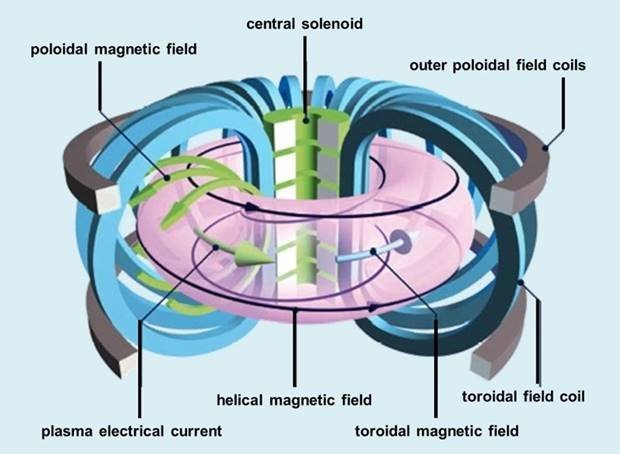
\includegraphics[width=10cm]{images/tokamak.jpg}
  \caption{A tokamak and relevant magnetic fields that create the helical particle trajectory \cite{tokamakSchema}.}
  \label{fig:tokamakSchema}
\end{figure}

Tokamak is a class of fusion devices whose name comes from the abbreviation of a Russian phrase which means ``toroidal chamber with magnetic coils''. It consists of a doughnut shaped vacuum chamber surrounded by powerful magnets that aim to confine a high temperature plasma that would otherwise damage the chamber. The plasma pressure and temperature are fundamental parameters in the context of nuclear fusion because they dictate the conditions required to overcome the electrostatic repulsion between positively charged atomic nuclei and bring them close enough for the strong nuclear force to initiate fusion reactions. In the core of stars like our Sun, the immense pressure and temperature generated by the gravitational collapse create the conditions where hydrogen nuclei (protons) can overcome their natural repulsion and fuse into helium, releasing a tremendous amount of energy in the process. To initiate fusion, hydrogen must be heated to temperatures in the range of 150 million Kelvin. In a tokamak, this is mainly accomplished with ohmic heating via a driving plasma current and neutral gas injection. This involves accelerating hydrogen ions to high speeds with electric fields and neutralising them the instant before they enter the chamber. The resulting plasma attains the required temperature, allowing nuclei to collide with sufficient energy for fusion reactions to occur. Figure \ref{fig:tokamakSchema} shows the position of various magnetic field coils within the tokamak. The toroidal magnetic field exerts an inward force on the plasma thus raising its pressure. High pressure is required to increase the frequency of collisions so that the energy output can exceed the large heating energy input. The central solenoid induces a current in the plasma which produces the majority of the poloidal magnetic field. This field is essential for confinement but it also plays a key role in plasma stability. The outer poloidal field coils can be controlled in real time to help mitigate instabilities. A real time inference of the electron density profile would assist in identifying instabilities and informing the algorithm that drives the control coils to mitigate them. In addition to high temperature and pressure, the tokamak design seeks to maximize the confinement time of the plasma. This is essential to allow a sufficient number of fusion reactions to occur before the plasma cools down or loses its stability. The magnetic fields in a tokamak are carefully optimized to prevent rapid plasma loss and minimize heat loss through various mechanisms, including turbulent transport. The shape of the density profile has a large effect on the confinement time.

The combination of the toroidal and poloidal fields shown in figure \ref{fig:tokamakSchema} creates a helical magnetic field within the plasma. Electrons and ions are accelerated in opposite toroidal directions by the central solenoid yet both follow a trajectory along the magnetic field lines. This is because a charged particle moving across a magnetic field succumbs to a force perpendicular to its motion. This causes them to gyrate around the magnetic field lines and confines them to follow the magnetic field lines. This is an oversimplification and in reality there are drift phenomina that cause the particles the deviate from following the magnetic field lines exactly. Collisions also cause deviations. A detailed description of particle motion within a magnetic field is not needed for this thesis. It is enough to know that the particles in general follow the helical path of the magnetic field lines with a small gyration around the field line. In many models used for data analysis the assumption that particles follow the magnetic field lines is used, including within this thesis. 

The magnetic field lines are confined to magnetic flux surfaces, figure \ref{fig:magfluxsurf}. The toroidal and poloidal flux is constant on magnetic flux surfaces, there is 0 flux across magnetic flux surfaces. Since we assume that the particles follow the magnetic field lines which are strictly bound to these surfaces, we also assume that the density is constant on these surfaces. This allows the density of the entire cross-section to be expressed with a 1D profile as a function of normalised radius $\rho$ for example, see \gls{nice}'s profile, figure \ref{fig:nice_example}. The normalised radius is constant at each flux surface. It is 0 at the magnetic axis and 1 at the plasma boundary. The magnetic axis is the very center point of the core and is defined as where the poloidal magnetic flux is minimum and the plasma boundary is the last closed flux surface. Particles past the plasma boundary are no longer bound and may interact with the plasma wall. The existence of nested magnetic flux surfaces shown in figure \ref{fig:magfluxsurf} rely on the ideal \gls{mhd} assumptions. Experiments frequently discover magnetic islands which discredits the assumption of nested flux surfaces. The electron density profiles inferred by \gls{nice} and this work make the nested flux surface assumption, although for many applications such as real time control, a highly accurate inference is often not required.

\begin{figure}
  \centering
  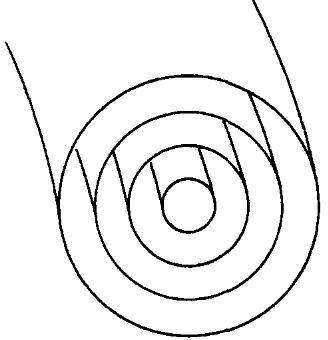
\includegraphics[width=5cm]{images/fluxsurf.png}
  \caption{Magnetic flux surfaces \cite{wessontokamak}.}
  \label{fig:magfluxsurf}
\end{figure}

\section{NICE}

\gls{nice} is an equilibrium reconstruction code that is routinely deployed for the \gls{west} tokamak. It is relevant because it computes an inference of the electron density profile that is available for comparison to the profile inferred in this work, although \glspl{nice} main objective is to infer the shape and position of the magnetic flux surfaces. \gls{nice} uses magnetic diagnostics. At \gls{west} these include 421 pickup coils, 36 flux loops and 12 Rogowski coils \cite{westmagdiag}. Magnetic diagnostics provide the majority of the information. \gls{nice} also uses interferometry, polarimetry, motional stark effect and pressure measurements. Equation \ref{eq:int_phase} and \ref{eq:pol_farad} further in the chapter, show how interferometry and polarimetry together can provide information about the poloidal magnetic field, which directly affects the magnetic flux and thus magnetic flux surfaces. \gls{nice} performs the inference by minimising a cost function. The cost function determines how well a physical state of the system matches the data received. A state is a specific position and shape of the magnetic flux surfaces and electron density profile. This requires a forward model. The forward model takes a state of the system and attempts to compute the signals that would be received by error free diagnostics if that state was the ground truth. The forward model is a simplified mathematical representation of the measurement process and can never be 100\% accurate. This introduces errors in the inference that need to be accounted for. The signals from the forward model can be compared to the actual signals received by the diagnostics to compute the cost function. By minimising the cost function the state that best matches the data is found. \gls{nice} uses \gls{sqp} as the minimisation algorithm. The optimal state of the system is then stored in the \gls{imas} database for \gls{west}. This includes the 1D electron density profile used as a comparison for the profile inferred in this work. \gls{nice} also imposes regularisation terms on their cost function. These penalise the cost function when state properties have features that disagree with prior knowledge. This includes smoothness. We expect the magnetic flux surfaces and electron density profile, to be continuous and smooth. A state inputted into the cost function that is not smooth triggers the regularisation term which causes the cost function to be larger. Minimising the cost function now also leads to smooth magnetic flux surfaces and electron density profile. This leads to a difficult question, how smooth should it be? \gls{nice} also have a regularisation term to penalise the cost function if the electron density profile is far from 0 at the last closed flux surface or plasma boundary. It is prior knowledge that the electron density is near 0 at the plasma boundary. How close to 0, and how strong should the regularisation be is still an open question. This work's approach has direct analogues to these regularisation terms. As explained later in more detail the length scale controls smoothness and an artificial observation ensures the density is close to zero at the plasma boundary. Figure \ref{fig:nice_example} shows an example of a \gls{nice} inferred electron density profile. It is modelled with a cubic spline function. It is the parameters of the cubic spline that are inputted into the cost function. The errors are calculated using a sensitivity method. In short, the error is deemed larger for the electron density of a particular normalised radius if a large change in the density leads to a small change in the cost function. In this case, we cannot be certain what density is better because many lead to a similarly low cost function and thus match the data similarly well. To include some more details, the \gls{sqp} minimisation algorithm computes the hessian of the cost function for minimisation, but this hessian can also be used to measure the sensitivity and thus the errors. The diagonal of the hessian contains the second differential of the cost function for each input parameter. This describes the curvature of the cost function in the direction of each parameter. A smaller curvature means a smaller sensitivity and thus a larger error.

\begin{figure}
  \centering
  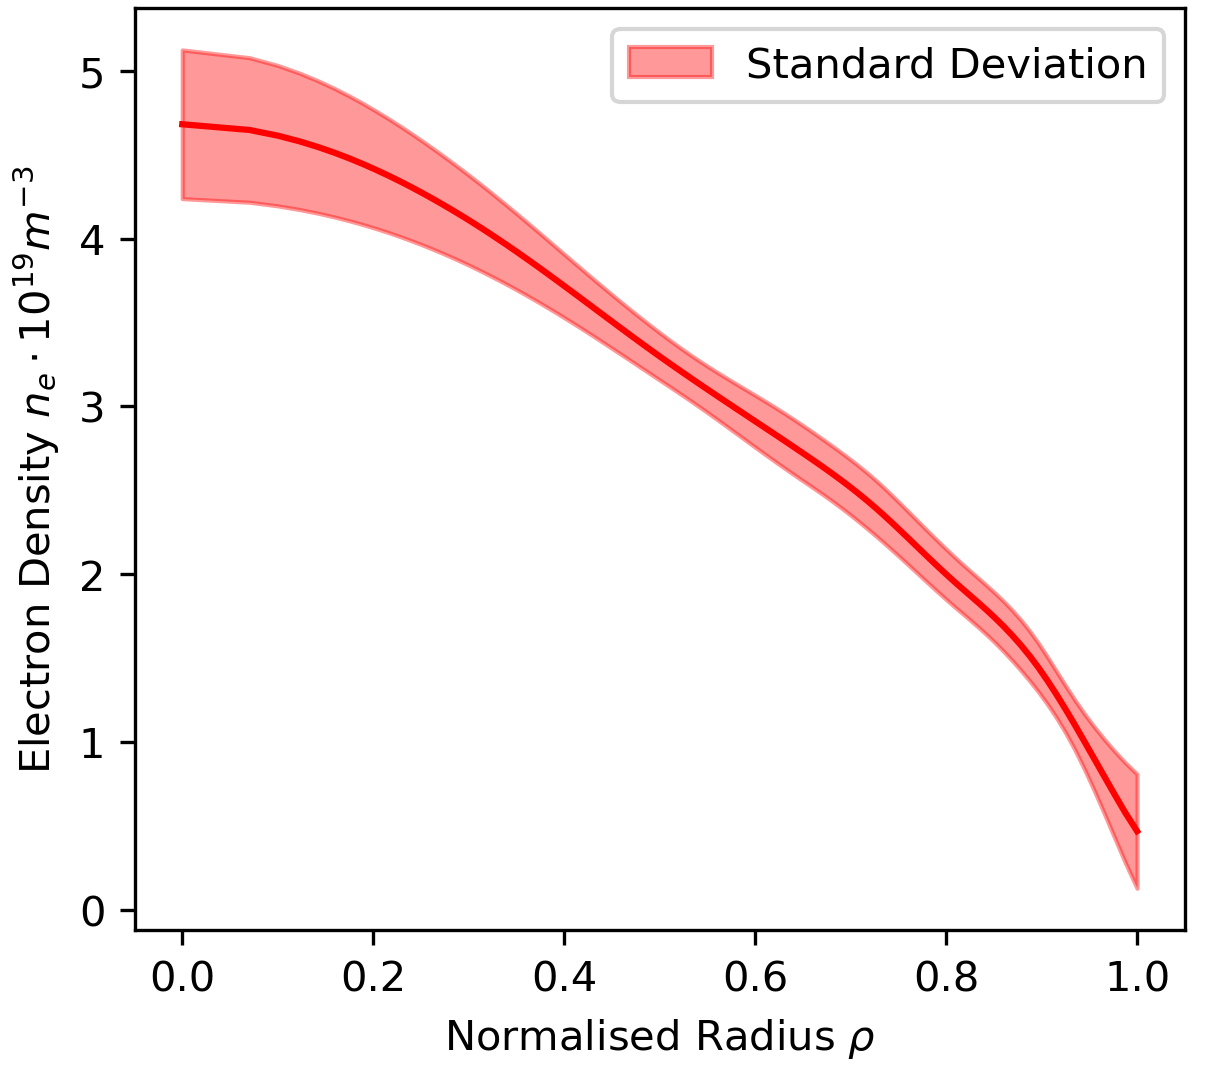
\includegraphics[width=13cm]{images/Final/nice.png}
  \caption{Electron density profile inferred by NICE for an instance in time within the WEST tokamak.}
  \label{fig:nice_example}
\end{figure}

\section{Bayesian Inference and the Simple Regression Problem}
\label{sec:BIandSRP}

This work aims to use Bayesian inference to obtain the electron density profile. Bayesian inference will be introduced generally and then it will be used to define a specific implementation applied to a simple regression problem. The method introduced will later be extended to solve the problem of inferring the electron density profile with interferometry data. The inferative Bayes' theorem for a physical quantity of interest $q$ is expressed as,

\begin{equation}
P(q|D,I) = \frac{P(D|q,I) P(q|I)}{P(D|I)},
\label{eq:bayesth}
\end{equation}

\noindent the posterior $P(q|D,I)$ is the probability density distribution of $q$ given the measured data $D$ and some prior information $I$. The $q$ that maximises the posterior is the most probable value of $q$ given the data and prior information. The uncertainty of $q$ can also be obtained from the posterior. The likelihood $P(D|q,I)$ is the probability density function that expresses the probability of the measured data given a fixed value of $q$ and the prior information. The likelihood is described by the experimental error for the data collection. The prior $P(q|I)$ contains information assumed about $q$ before the data is taken. The marginal likelihood or evidence $P(D|I)$ is simply the probability of the data given the prior information only. For posterior computation, the marginal likelihood serves as a normalisation factor. Normalisation is often carried out with other means to simplify the posterior computation. Although the marginal likelihood can be used to tune hyperparameters; as will be shown later.

The version of Bayes' theorem for a simple 1D regression problem is,

\begin{equation} 
  P(\vec{y}|\vec{d},\vec \epsilon, \theta) = \frac{P(\vec{d}|\vec{y},\vec \epsilon) P(\vec y|\theta)}{P(\vec d|\vec \epsilon, \theta)},
  \label{eq:bayesth_simple_regression}
\end{equation}

\noindent where $\vec y$ contains the values of a curve at regular $x$ values. The goal is to find the most likely $\vec y$ given the data and prior information. $\vec d$ contains curve measurements at known $x$ values with some experimental errors $\vec \epsilon$. $\theta$ is a set of parameters related to the prior form, explained more later. The likelihood and prior are going to be clearly defined as multivariate Gaussians giving a multivariate Gaussian posterior which needs to somehow model the curve $\vec y$. Figure \ref{fig:mvg} illustrates how a multivariate Gaussian can model a curve. The functional form of a multivariate Gaussian is,

\begin{equation}
  \mathcal{N}(\vec y, \vec{\mu}, \Sigma) = \frac{1}{\sqrt{(2\pi)^{\frac{n}{2}}|\Sigma|}} \exp \left[{{-\frac{1}{2}(\vec{y}-\vec{\mu})^T\Sigma^{-1}(\vec{y}-\vec{\mu})}}\right],
  \label{eq:mvg}
\end{equation}

\noindent the mean vector $\vec{\mu}$ holds the $y$ values of the curve at regular intervals along the $x$ axis. The diagonal of the covariance matrix holds the squared standard deviations of each Gaussian within the multivariate. These will be used to represent of the uncertainty of the curve inferred from the data. Figure \ref{fig:mvg} shows 10 Gaussians with each mean connected by a straight line. In practice, many Gaussians are used in a small space so that even a linear interpolation appears as a smooth curve. In our simple regression problem 101 Gaussians are used, thus $\vec y$ has a length of 101. 

For the simple 1D regression problem the posterior distribution is a multivariate Gaussian that represents the most likely curve given the data and prior information, see figure \ref{fig:srpvis} for a visualisation. It can be expressed as,

\begin{figure}
  \centering
  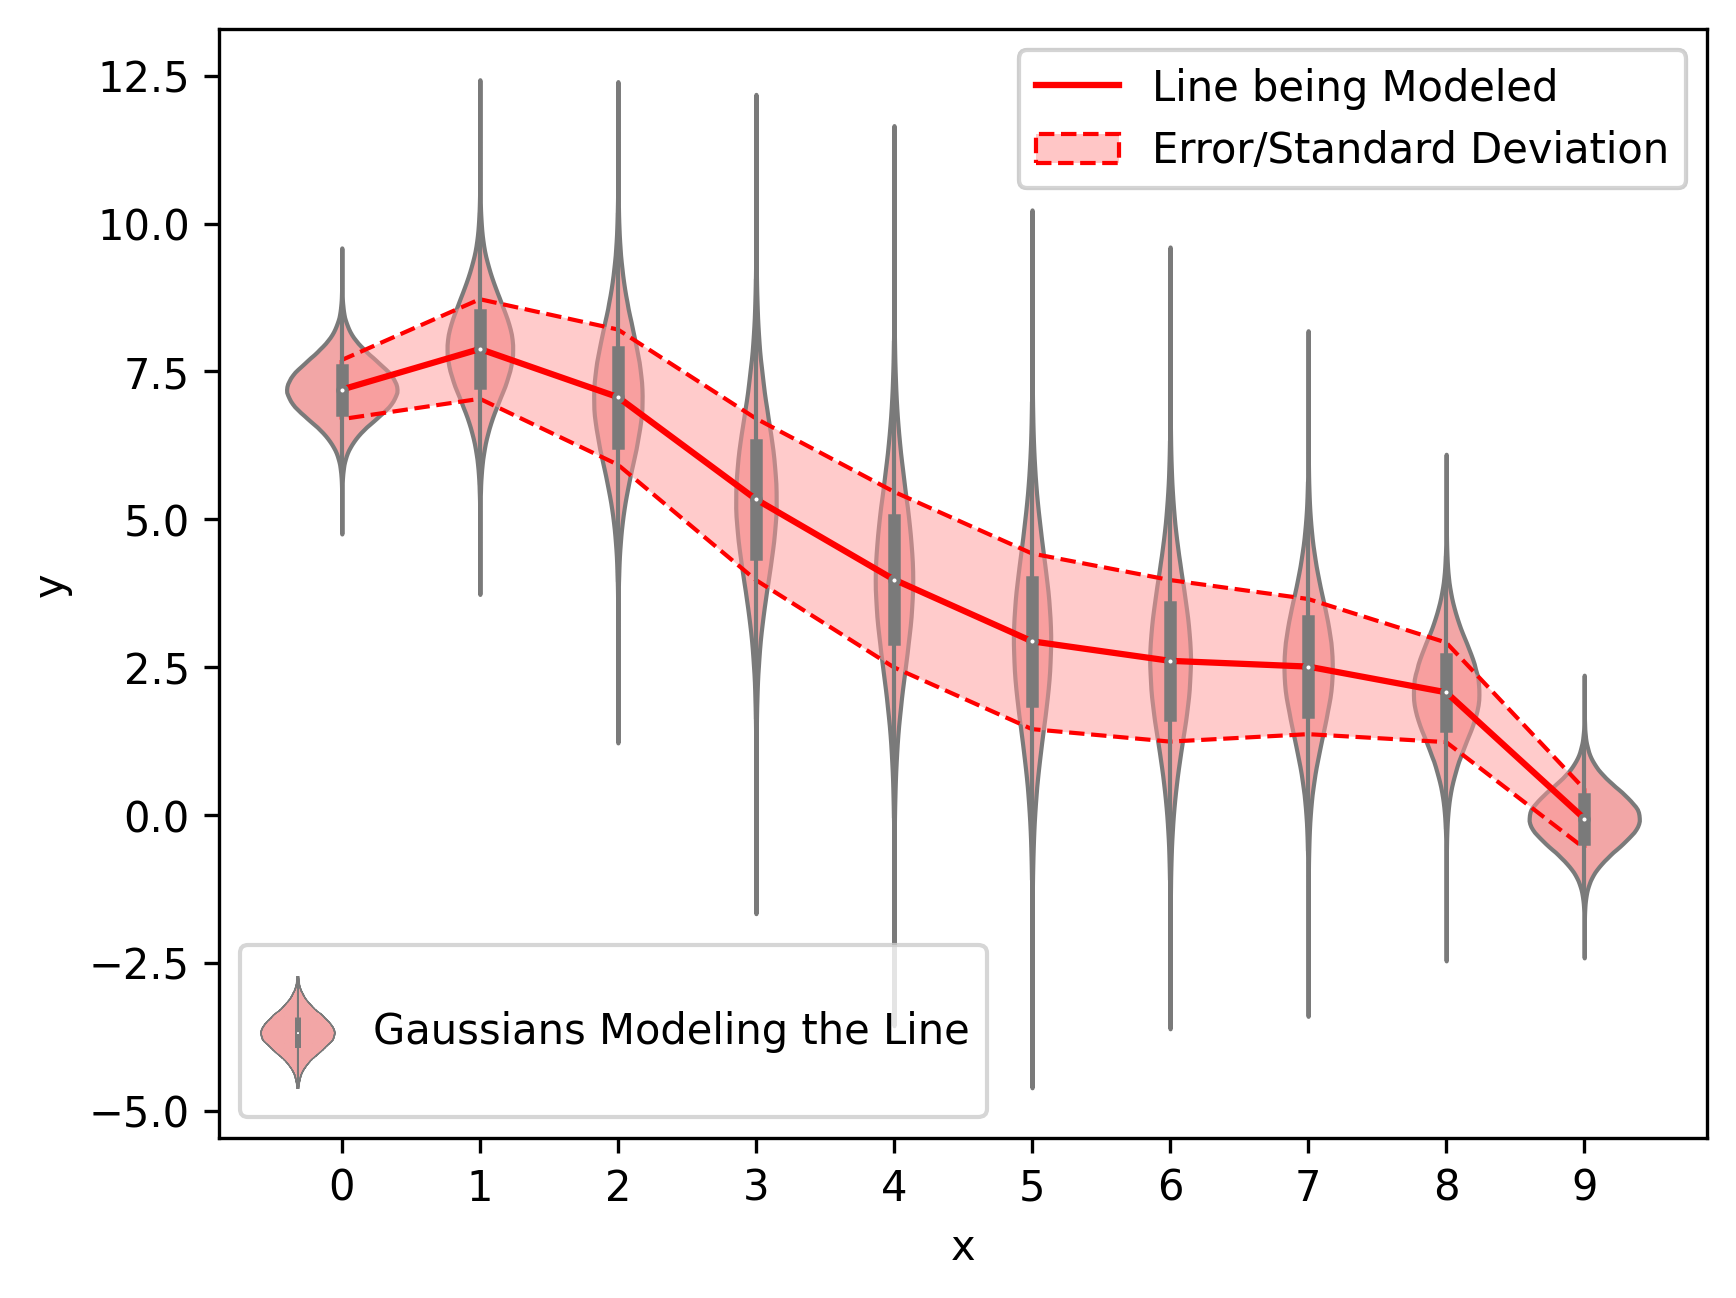
\includegraphics[width=10cm]{images/mvg.png}
  \caption{Illustrating how many Gaussians can model a curved line and its uncertainty.}
  \label{fig:mvg}
\end{figure}

\begin{equation}
  \mathcal{N}(\vec y, \vec{\mu}_{post}, \Sigma_{post}),
\end{equation}

\noindent where $/vec{\mu}_{post}$ has a length of 101, the same as the unknown $y$ values. To compute $\mu_{post}$ and $\Sigma_{post}$ we must define the likelihood and prior. If $m$ measurements are taken the likelihood is defined as, 

\begin{equation}
  P(\vec{d}|\vec{y},\vec \epsilon) = \mathcal{N}(\vec{d}, \vec \mu_{li} = R\vec{y}, \Sigma_{li}),\, \Sigma_{li} = \vec{\epsilon}I = 
    \begin{bmatrix}
        \epsilon_1 & 0 & \hdots & 0\\
        0 & \epsilon_2 & \hdots & 0\\
        \vdots & \vdots & \ddots & 0 \\
        0 & 0 & 0 &\epsilon_m
    \end{bmatrix},
  \label{eq:likelihood}
\end{equation}

\noindent where $R$ is the response matrix. Given some curve $\vec y$ to be true, $R \vec y$ is a vector that has the same length as $\vec d$ and contains the values of the curve $\vec y$ at the same $x$ values that the data was collected at. The response matrix is an error free model of the measurement process. In the likelihood of figure \ref{fig:srpvis} the blue line is an example of a given $\vec{y}$ and if this was the ground truth and we took an error free measurement at the same $x$ points as our original data then we would get the points indicated by the mean of each Gaussian. These points are computed with $R\vec y$ and provide the mean vector of the likelihood. The likelihood represents the probability of getting the black data points given the blue line $\vec y$ is the ground truth. Regression is inherently an inverse problem and the response matrix is a forward model. 

Here is is worth noting what a Gaussian process is and how a multivariate Gaussian is an approximation of it. A Gaussian process is a stochastic process that can be represented by a multivariate Gaussian of infinate dimensions. For example the $x$ variable in \ref{fig:srpvis} is continuous and thus has infinate values between $0$ and $9$. The curve that best fits the data is made of an infinate number of points, each point with an uncertainty. This can be modeled with an infinate number of Gaussians and thus the posterior can be said to be a Gaussian process. Since infinate precision is not possible with a computer a many dimension multivariate Gaussian is used, which is an approximation of the Gaussian process. Regression carried out with Bayesian inference and a Gaussian process prior is often referred to as Gaussian Process Regression; even when the finite dimension multivariate Gaussian approximation is used. The prior for this simple regression problem is a multivariate Gaussian. Although, the method being introduced is more general than the typical implementation of Gaussian Process Regression. This is so that it can easily be extended later to allow regression in situations where the data resides in a different space. To avoid confusion with the typical version of Gaussian Process Regression the term is not used for this implementation. For an introduction to typical Gaussian Process Regression, I suggest the textbook Gaussian Processes for Machine Learning \cite{gp4ml}. The prior can be defined as,

\begin{equation}
  \mathcal{N}(\vec{y}, \vec \mu_{pr} = \vec{0}, K), \, K_{ij} = k(x_i, x_j) = \sigma^2 \exp\left[{\frac{(x_i - x_j)^2}{2l^2}}\right], 
  \label{eq:prior}
\end{equation}

\noindent where $\vec 0$ is a vector of 101 zeros, the same length as $\vec y$. The zero vector is a commonly used `non-informative' prior mean vector. The covariance matrix $K$ is constructed using the kernel $k(x_i,x_j)$. The main role of the amplitude, $\sigma$, in the kernel is to set the prior strength. A high amplitude means the inference has a low prior strength and the resultant curve can be far from the prior mean $\mu_{pr} = \vec 0$. See the prior in figure \ref{fig:srpvis}, the amplitude $\sigma$ is the standard deviation of these Gaussians shown. For visualisation purposes only 5 prior Gaussians are shown in figure \ref{fig:srpvis}, yet in reality there are 101, the same number as there are unknown $y$ values. The length scale, $l$ sets the strength of the correlation between the Gaussians. A low length scale means that only Gaussians close in $x$ are highly correlated. Gaussians further in $x$ would have a low correlation, meaning they can have a very different mean value. A low length scale allows the fitted curve to have more complexity similar to a high order polynomial and can lead to overfitting. A high length scale limits the fit's ability to curve sharply leading to a simple model, similar to a low order polynomial, leading to underfitting. A very high length scale leads to an almost linear fit. This prior is far from perfect. For instance, it is often known that the inferred values must be positive as you cannot have a negative electron density. Since the prior mean vector is set to $\vec{0}$, a negative value is as likely to be inferred as a positive value. Since it is Gaussian, values close to 0 are more likely to be inferred than values far from 0. To mitigate this a high amplitude can be used to lower the prior strength and allow the data in the likelihood to have more influence on the posterior result. The kernel $k(x_i,x_j)$ in equation \ref{eq:prior} is known as the exponential square kernel. It is a very commonly used kernel but far from the only choice. The single value of the length scale prevents the inference from having long smooth regions with few features followed by regions of high variability. This can be an issue when inferring H-mode tokamak plasmas that have a sharp drop-off in density at the plasma edge. For these situations, a non-stationary kernel can be used that allows the length scale to be a function of $x$ which can then allow for posteriors of varying complexity. Regardless of the kernel used, deciding the optimal values of its parameters for a problem is not obvious and various options will be explored. 

\begin{figure}[H]
  \centering
  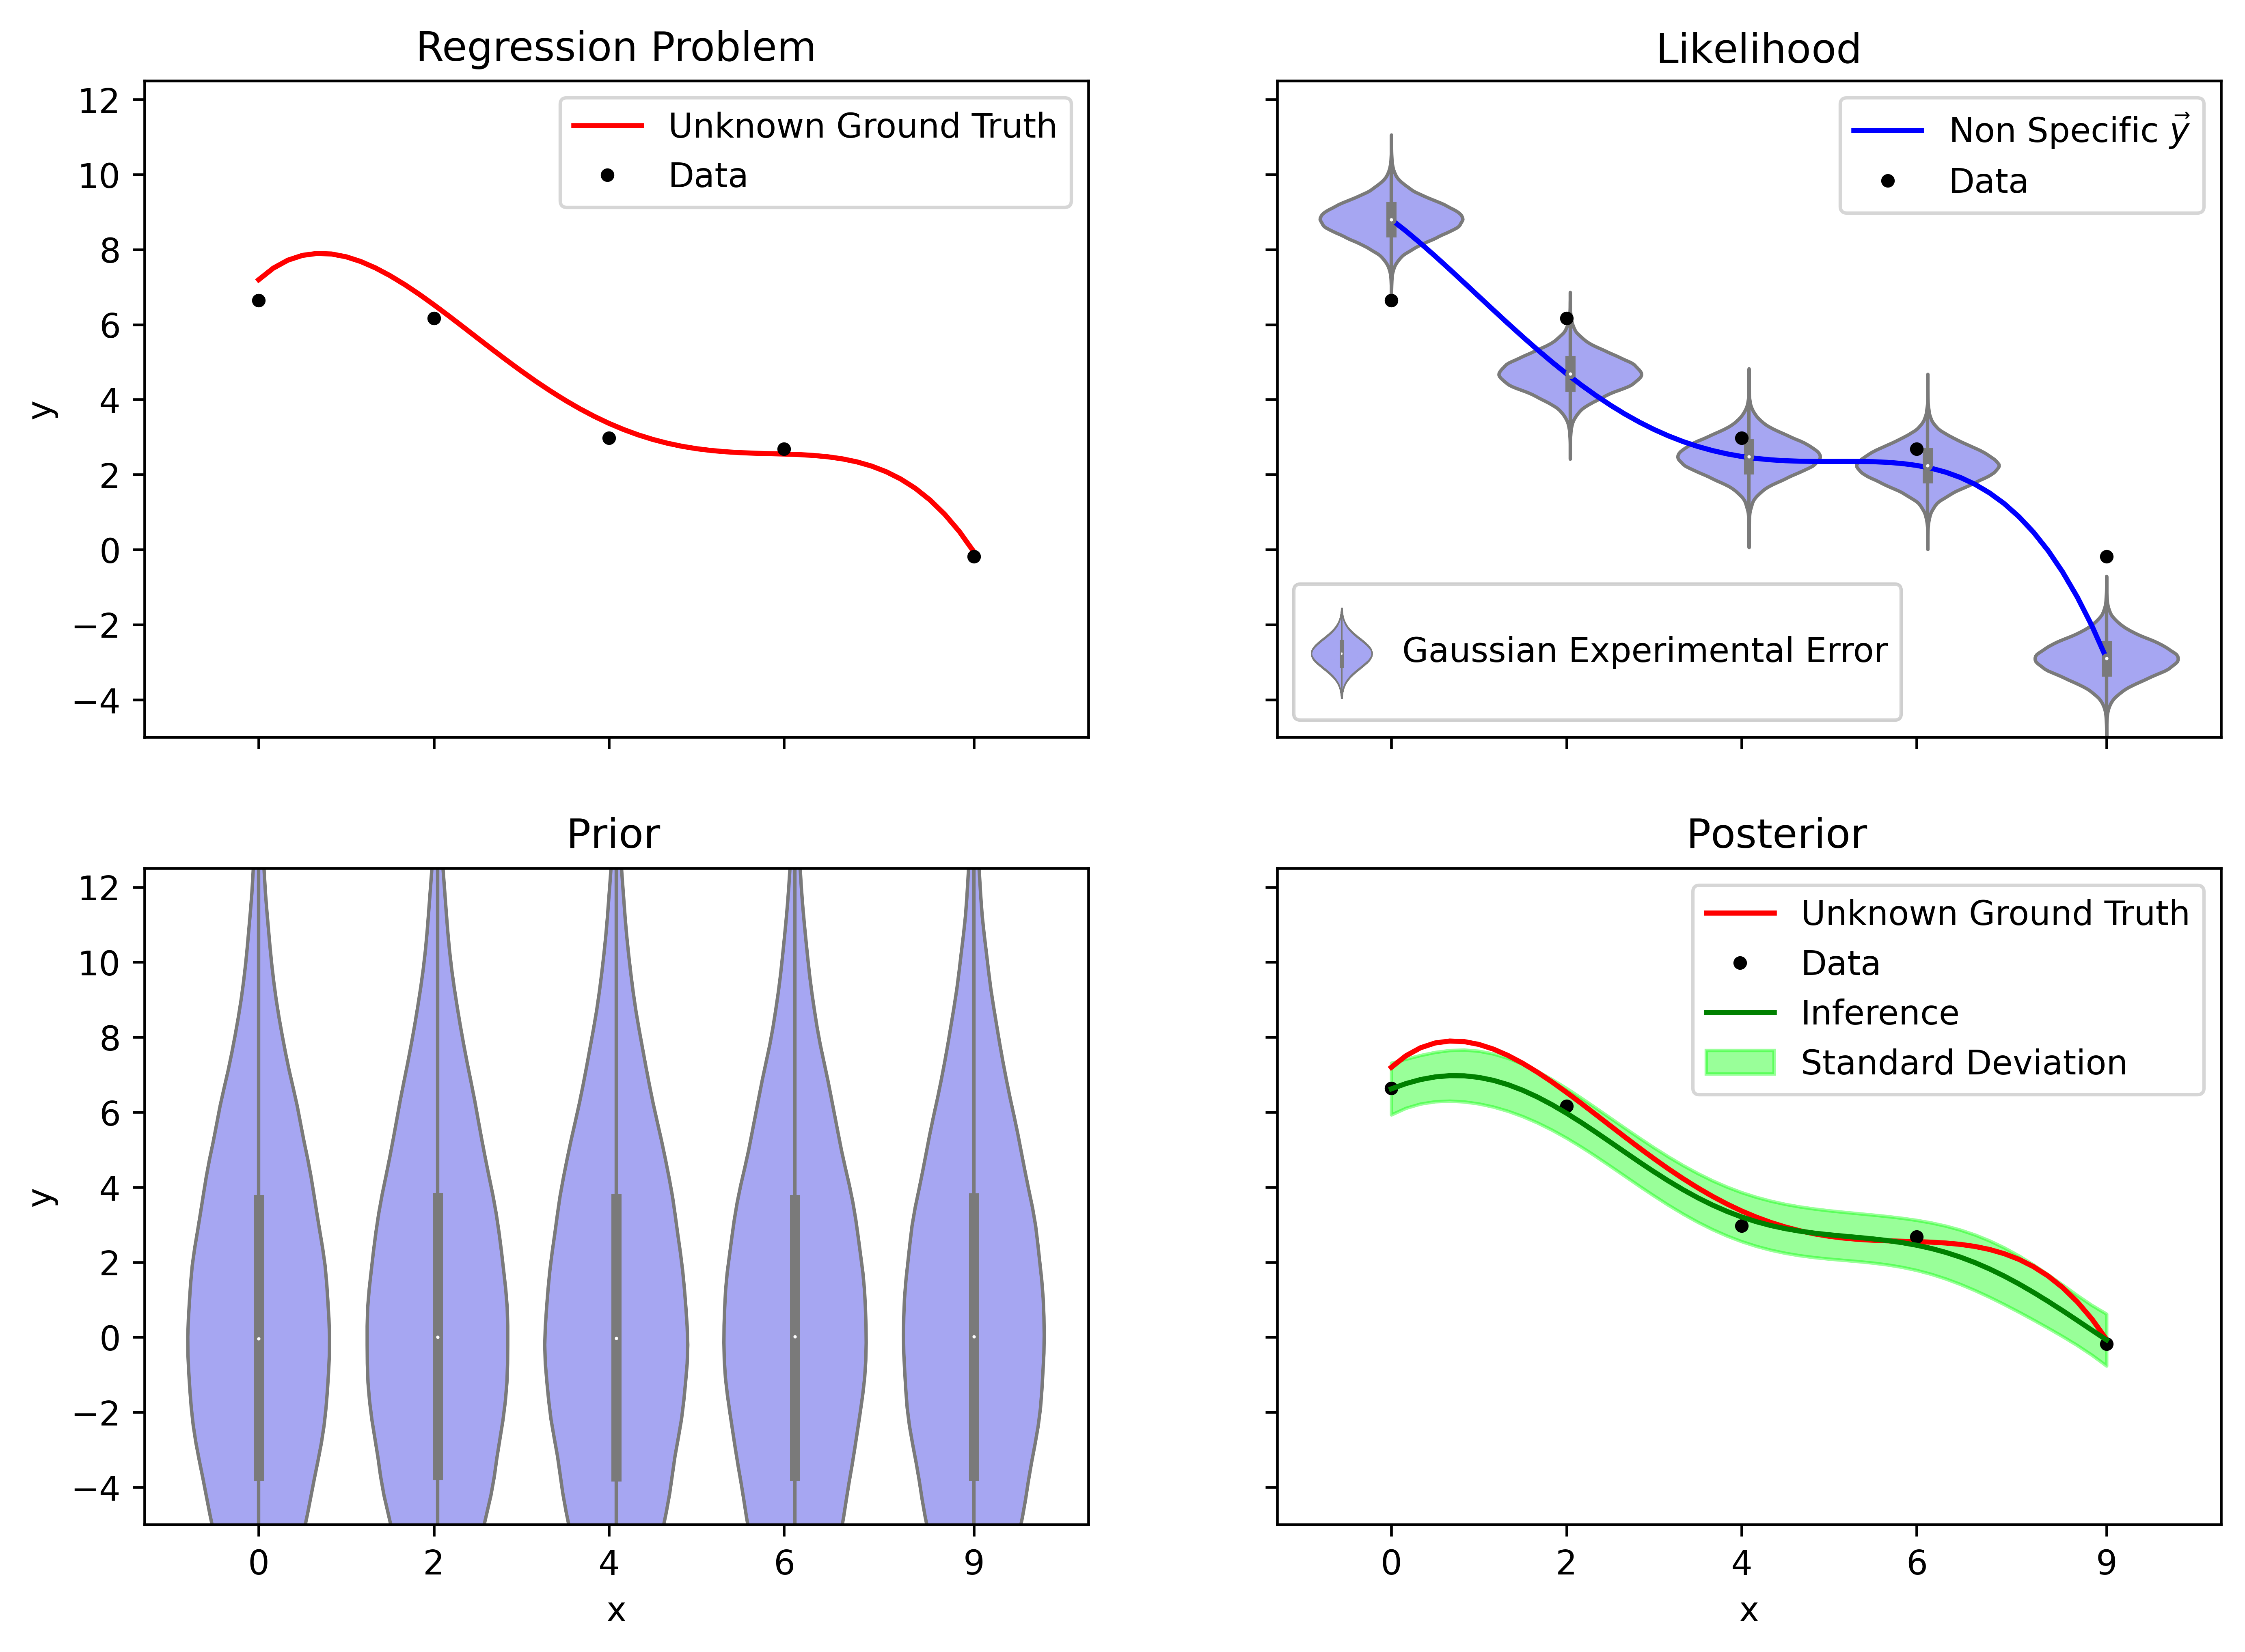
\includegraphics[width=13cm]{images/srpvis.png}
  \caption{A visualisation of the simple regression problem and the various distributions involved in the Bayesian inference solution.}
  \label{fig:srpvis}
\end{figure}

Figure \ref{fig:srpvis} shows the simple regression problem, it then tries to show the Gaussians that make up the likelihood and prior although it is not perfect. We assume the observations are independent giving the likelihood a diagonal covariance matrix. So the multiple Gaussians that make up the likelihood are not dependent on each other, thus representing them individually provides all the information in the likelihood. The prior has a more complex covariance matrix $K$, and figure \ref{fig:srpvis} does not have a complete representation of the priors form. Figure \ref{fig:srpvis} also shows the 101 Gaussians that make up the posterior by plotting the regularly spaced $\vec{\mu}_{post}$ values in green with a green shadow showing the standard deviations of each Gaussian that are found in the diagonal of $\Sigma_{post}$. The posterior mean vector and covariance matrix can be computed with the closed form expressions,

\begin{align}
\label{eq:mupost}
\vec{\mu}_{post} &= \vec{\mu}_{pr} + (K^{-1} + R^{\top} \Sigma_{li}^{-1} R)^{-1} R^{\top} \Sigma_{li}^{-1} (\vec{d} - R \vec{\mu}_{pr}),\\
\label{eq:covpost}
\Sigma_{post} &= \left(R^\top \Sigma_{li}^{-1} R + K^{-1}\right)^{-1},
\end{align}

\noindent which are derived in appendix \ref{append:dervcf}. The main steps include multiplying the functional forms of the prior and likelihood, ignoring all scaling factors, simplifying until they form a single unnormalised multivariate Gaussian and then comparing this with the posterior. 

There is still the issue of deciding the values of the hyperparameters to place in $K$ and the experimental error to place within $\Sigma_{li}$. Often the experimental error is not precisely known and can also be treated as a hyperparameter. To select the hyperparameters we can perform a separate hyperparameter Bayesian inference,

\begin{equation}
  P(\theta, \vec{\epsilon}|\vec d) = \frac{P(\vec d|\theta, \vec{\epsilon}) P(\theta,\vec{\epsilon})}{P(\vec d)},
  \label{eq:parambayes}
\end{equation}

where the most probable hyperparameters given the same data can be found by maximising the hyperparameter posterior, $P(\theta,\vec{\epsilon}|\vec d)$. This method is known as \gls{map}. Notice the likelihood $P(\vec d| \theta, \vec{\epsilon})$ is exactly the marginal likelihood from the inferative Bayesian formula \ref{eq:bayesth}. The prior $P(\theta, \vec{\epsilon})$ needs to accurately represent our prior knowledge of the hyperparameters. By maximising the numerator of Bayes theorem the posterior is also maximised. The marginal likelihood from the hyperparameter Bayes theorem $P(\vec d)$, can safely be ignored as it is a normalisation constant. All further mentions of marginal likelihood refer to the inferative distributions marginal likelihood $P(\vec d|\theta,\vec{\epsilon})$; as is the usual terminology for this procedure. It can be computed by integrating the numerator of the inferative Bayesian over the quantity of interest:

\begin{equation}
  \begin{aligned}
   P(\vec d|\vec\epsilon,\theta) &= \int P(\vec{d}|\vec{y},\vec\epsilon)P(\vec{y}|\theta)  \, d\vec y \\
   &= \frac{1}{(2\pi)^{\frac{m}{2}} \sqrt{|\Sigma_{li} + RKR^\top|}} \exp\left[ -\frac{1}{2} (\vec{d} - R\vec{\mu}_{pr})^{\top} (\Sigma_{li} + R K R^{\top})^{-1} (\vec{d} - R\vec{\mu}_{pr}) \right].
   \label{eq:margeli}
  \end{aligned}
\end{equation}

\noindent The values of the marginal likelihood can become very large and troublesome to compute with standard 64-bit float precision. For this reason, the logarithm is computed. It is the convention when performing optimisation to define a loss function to be minimised, thus the negative log marginal likelihood is used. Scaling constants do not affect the minimum value and can be ignored. The negative log marginal likelihood used as a loss function for hyper-parameters is then,

\begin{equation}
loss(\vec \epsilon,\theta) = \ln(|\Sigma_{li}+RKR^\top|) +  (\vec{d} - R\vec{\mu}_{pr})^{\top} (\Sigma_{li} + R K R^{\top})^{-1} (\vec{d} - R\vec{\mu}_{pr}),
\label{eq:loss}
\end{equation}

\noindent the full derivation of this expression can be found in appendix \ref{append:dervml}. To include a uniform prior for the hyperparameters $P(\theta, \vec{\epsilon})$, the loss function can be programmed to return infinity (or a very large number) when the proposed hyperparameters are outside their bounds. Although some minimisation algorithms can avoid proposing values outside of determined bounds.

An alternative solution is to perform a full Bayesian analysis where the hyperparameters are marginalised out of the inferative posterior. This allows the inferative posterior to become independent of the hyperparameters and allows for a more robust and flexible inference. Marginalisation of the posterior can be written as,

\begin{equation} 
  P(\vec{y}|\vec{d}) = \int \int P(\vec y, \theta, \vec \epsilon|\vec d) \, d\theta \, d\vec \epsilon ,
\end{equation}

and with conditional probability rules,

\begin{equation}
  P(\vec{y}|\vec{d}) = \int \int P(\vec y | \theta, \vec \epsilon, \vec d) P(\theta, \vec \epsilon|\vec d) \, d\theta \, d\vec \epsilon.
\end{equation}

Notice that $P(\vec y|\theta, \vec \epsilon)$  is our original inferative posterior and $P(\theta, \vec \epsilon|\vec d)$ is the hyperparamter posterior from earlier. Sampling $y$ from the joint distribution $P(\vec y|\theta, \vec \epsilon) P(\theta, \vec \epsilon|\vec d)$ is equivalent to sampling from the posterior $P(\vec y|\vec d)$, that does not depend on the hyperparameters. To accomplish this a first step is to use \gls{mcmc} sampling techniques to sample $\theta$ and $\vec \epsilon$ from the hyperparameter posterior. This only requires the ability to compute the log of the hyperparameter likelihood and prior given a proposed set of hyperparameters. The prior is defined by us and so must be computable and the likelihood is exactly the inferative marginal likelihood and has an analytical form given previously in equation \ref{eq:margeli}. MCMC sampling involves initalising at a random position in the parameter space and using a stochastic proposal function to suggest a new position given the current position. If the new position satisfies the Metropolis Hastings criterion, it is accepted and the values of the hyperparameters at the new position are collected as a sample. Otherwise the sample is rejected and the proposal distribution suggests a new position. After some number of iterations, the samples closely represent samples from the true posterior. The first few samples are usually a poor representation of the posterior, especially if they are initialised far from the posterior maximum. For this reason, the first few samples are often discarded as a burn in. The final samples of $\theta$ and $\vec \epsilon$ can be used to sample $\vec y$ from the inferative posterior $P(\vec y|\theta, \vec \epsilon)$; which is a multivariate Gaussian of mean and covariance given by equations \ref{eq:mupost} and \ref{eq:covpost}. Sampling from a known multivariate Gaussian can be done with more simple sampling techniques that have zero possibility of sample rejection: \gls{mcmc} sampling is not required. Remember that each sampled $\vec y$ is a curve where the vector items correspond to $y$ values of the curve at regularly spaced $x$ intervals; as shown in figure \ref{fig:srpvis}. Thus the most likely value of the curve is the mean or median of the posterior samples at each $x$ value. For uncertainty, the standard deviation of certain quantiles can be computed.marginal likelihood

This thesis uses the Python package emcee for the \gls{mcmc} sampling. This involves initialising a group of `walkers' at random parameter positions. They then explore the space of the provided posterior distribution using a proposal function and the Metropolis-Hastings criteria. The proposal function suggests a new position in the hyperparameter space based on the current position.

An additional caveat of \gls{mcmc} sampling is that the samples from a walker's chain are autocorrelated, yet a true sample from the posterior would not depend on the current position of a walker. To reduce autocorrelation the chains are often thinned. Thinning by a degree of three means removing every third sample. This reduces autocorrelation and the samples more accurately represent samples from the posterior. Over-thinning limits the number of samples obtainable with the given computation power and time limits, leading to a loss of precision of the inference. To aid in deciding the thinning degree one can compute the \gls{iat}. This is a measure of how many steps it takes for a Markov chain to forget its initial state and become uncorrelated. Thinning by a degree of the \gls{iat} will ensure there is almost no autocorrelation between the samples but this is extreme and often means very long run times for a few samples that produce much less precise results than if more samples are kept.

Another way to reduce autocorrelation is to tune the \gls{mcmc} algorithms hyperparameters. The proposal function often has tunable parameters. The choice of prior also plays a major role.

\section{Interferometry and Polarimetry}

\begin{figure}[H]
  \centering
  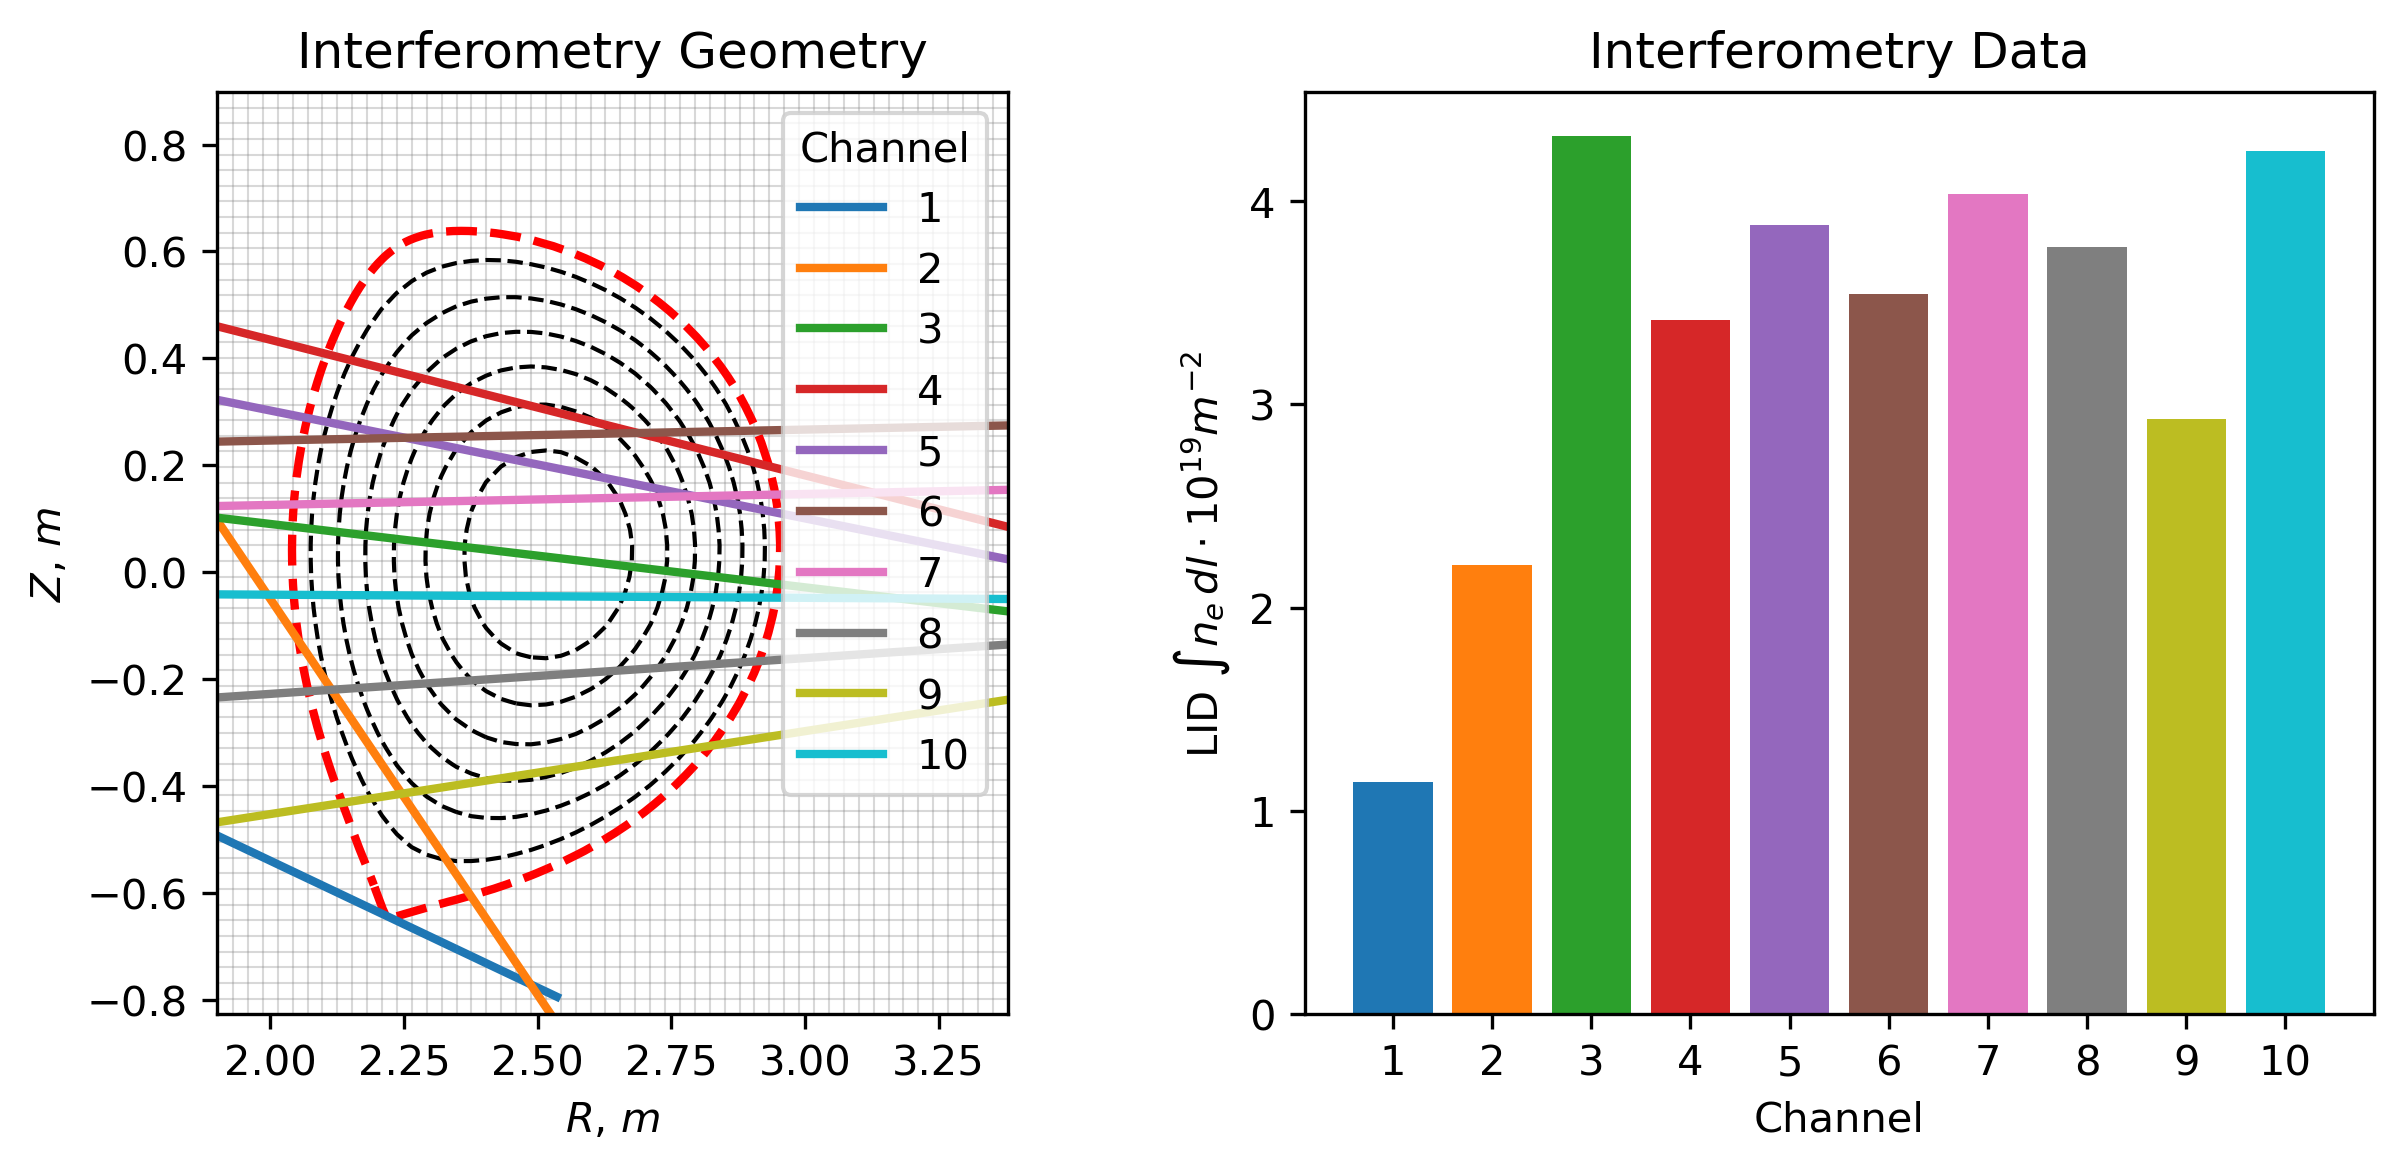
\includegraphics[width=15cm]{images/54344_7s_interf.png}
  \caption{Polodial cross section showing the geometry of interfero-polarimetry lasers at WEST \cite{westinterfero} and some example interferometry data.}
  \label{fig:interfgeo}
\end{figure}

Interferometry and Polarimetry are techniques that use the interference of electromagnetic waves to measure the properties of a medium. Interfero-polarimetry lasers within a tokamak penetrate the plasma at various angles. The geometry at \gls{west} is shown in figure \ref{fig:interfgeo}. Each laser is split into two beams: one that passes through the plasma and one that bypasses it. The two beams are then recombined and detected by a receiver. The phase difference between the two beams depends on the difference in the optical path length, which is affected by the electron density along the line of sight. Interferometry measures the phase difference; allowing one to calculate the line integrated electron density of the plasma $\int n_e \, dl$, 

\begin{equation} 
  \label{eq:int_phase}
  \Delta\phi = \frac{\lambda e^{2}}{4 \pi \epsilon_0 m_e c^2 } \int n_e \, dl \, \cite{princPlasDiag}.
\end{equation}

\noindent The laser wavelength $\lambda$, is combined with other common physical constants to ascertain the constant of proportionality. \gls{west} has stored the line integrated electron density as raw interferometry data in the \gls{imas} database. This is the data that will be used for this work. Although there is not enough information to completely and accurately reconstruct the electron density profile a best guess given the data can be inferred.

Polarimetry measures the Faraday rotation angle of the lasers. The linearly polarised lasers experience a rotation as the circularly polarised components travel through the plasma at different speeds. This is due to the small gyration of the electrons around the magnetic field. The Faraday rotation angle is proportional to the line integrated density of $n_e B_{||}$ along the line of sight of the lasers, 

\begin{equation}
  \label{eq:pol_farad}
  \theta_F = \frac{\lambda^2 e^3}{8 \pi^2 c^3 \epsilon_0 m_e^2} \int n_e B_{||} \, dl \, \cite{princPlasDiag},
\end{equation}

\noindent where $B_{||}$ is the magnetic field strength parallel to the line of sight. Polarimetry has information about electron density and this work could be extended to become a Bayesian integrated analysis which includes this information in the inference. Only interferometry information is used in this thesis. Polarimetry can be used in combination with interferometry to gain information about the poloidal magnetic field and this is why \gls{nice} uses it to determine the position of the magnetic flux surfaces.

\section{Bayesian Inference for Interferometry}\label{sec:InfForInterf}

To infer the electron density profile with interferometry, the previously defined regression process is altered. $\vec{y}$ becomes $\vec{n_e}$, the $\vec{0}$ prior mean can remain the same. The amplitude $\sigma$ and length-scale $l$ can be re-optimised by maximising the marginal likelihood. The data is now in a different space and thus is the likelihood. The response matrix $R$ must be created so that it will transform a profile $\vec{n_e}$ into what would be measured by an error free version of the \gls{west} interferometry system given $\vec{n_e}$ is the true profile. The result of $R \vec{n_e}$ is a vector the same length as the data $\vec{d}$ where each element corresponds to a different interferometry laser or channel. 

The response matrix computation can be summarised in a few steps. \Gls{nice} provides the magnetic flux at a set of grid points on the tokamak poloidal cross-section. It also provides the flux at a set of flux surfaces. The normalised radius $\rho$ of each flux surface is known. A simple 1D interpolation can be used to determine the normalised radius at each grid point. Then using $\vec{n_e}$ another 1D interpolation can be done to determine the electron density at each grid point. After the density at any point along a laser's line of sight $n_e(l_i)$, can be computed using triangular mesh interpolation. The density at the golden cross in figure \ref{fig:meshtriangle} can be computed as a weighted sum of the density at the three nearest grid points $\{g_1, g_2, g_3\}$ that form the golden triangle,

\begin{figure}
  \centering
  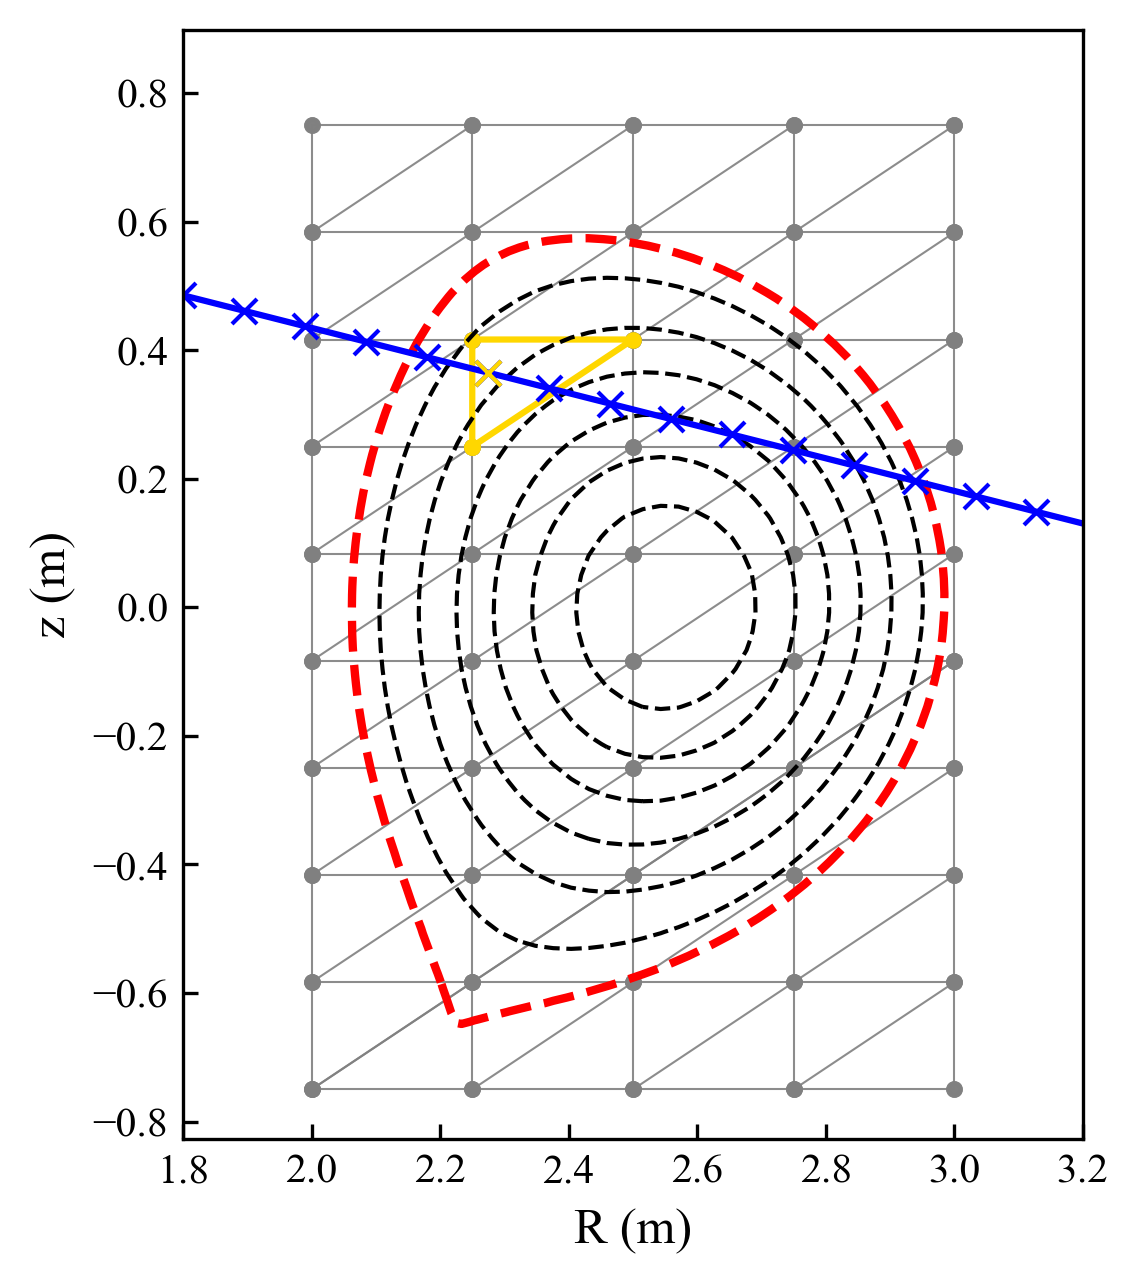
\includegraphics[width=10cm]{images/meshtriangle.png}
  \caption{An example mesh grid to aid visualisation of the triangular mesh grid interpolation used in the response matrix construction.}
  \label{fig:meshtriangle}
\end{figure}

\begin{equation}
  n_e(l_i) = \lambda_1 n_e(g_1) + \lambda_2 n_e(g_2) + \lambda_3 n_e(g_3),
\end{equation}

\noindent where $\lambda$ values can be computed using the $(R_1,z_1), (R_2,z_2), (R_3,z_3)$ coordinates of the 3 known density points and the point of interest $(R, z)$,

\begin{gather}
\lambda_1 = \frac{(z_2 - z_3)(R - R_3) + (R_3 - R_2)(z - z_3)}{(z_2 - z_3)(R_1 - R_3) + (R_3 - R_2)(z_1 - z_3)},\\
\lambda_2 = \frac{(z_3 - z_1)(R - R_3) + (R_1 - R_3)(z - z_3)}{(z_2 - z_3)(R_1 - R_3) + (R_3 - R_2)(z_1 - z_3)},\\
\lambda_3 = 1-\lambda_1-\lambda_2.
\end{gather}

\noindent These $\lambda$ values are known as the barycentric coordinates of the point of interest. The line integrated density can be approximated as a sum of electron densities at many points along the line of sight, $l_i$, times the width of their separation $\Delta l$,

\begin{equation}
  \int n_e \, dl \approx \sum_i n_e(l_i) \Delta l.
  \label{eq:neapprox}
\end{equation}

\noindent The contribution $w(g_i)$ of each grid point $g_i$ is a sum of all the mesh interpolation coefficiants $\lambda_j$ used on that point,

\begin{equation}
  \int n_e \, dl \approx \Delta l \sum_i w(g_i) n_e(g_i), \, w(g_i) = \sum_j \lambda_j.
\end{equation}

\noindent Each point can be associated with the nearest flux surface $f_i$ equally spaced in $\rho$. This way the contribution $w(f_i)$ of each flux surface is a sum of the contribution at each of its associated grid points $g_j$,

\begin{equation}
  \int n_e \, dl \approx \Delta l \sum_i w(f_i) n_e(f_i), \, f = \sum_j g_j.
  \label{eq:neapproxFS}
\end{equation}

\noindent All of these steps equate to a simple re-ordering of the original summation \ref{eq:neapprox} to extract the contribution of each flux surface on the final integrated density value. Equation \ref{eq:neapproxFS} can be computed using a vector product,

\begin{equation}
  \int n_e \, dl \approx \Delta l \vec{w}^{\top} \vec{n_e}.
\end{equation}

\noindent The contribution vector applies to one line of sight. The computation for all lines of sight can be performed by placing the $\Delta l \vec{w}$ vector for each line of sight as a row in the response matrix $R$. Thus, a vector of line integrated densities for the likelihood can be created,

\begin{equation}
  \vec{\mu_{li}} = R \vec{n_e}.
\end{equation}

\noindent This responce matrix $R$ can then be used in the closed form expressions \ref{eq:mupost} and \ref{eq:covpost}, to perfrom a 1D electron density profile inference.

Some further alterations to the inference method can be made to further increase reliability. These include altering the kernel and adding artificial observations to include prior knowledge. The kernel can be changed to a non-stationary kernel, 

\begin{equation}
  K_{ij} = k(\rho_i, \rho_j) = \sigma^2 \left( \frac{2l(\rho_i)l(\rho_j)}{l(\rho_i)^2 + l(\rho_j)^2} \right)^{1/2} \exp\left(-{\frac{(\rho_i - \rho_j)^2}{l(\rho_i)^2+l(\rho_j)^2}}\right),
\end{equation}

\noindent this allows the length scale to change as a function of $\rho$. The length scale controls smoothness, model complexity and curvature. If these are free to change for different regions of the plasma then there is a greater range of possibilities for the final inference. A cubic spline function can be used for significant flexability. This is where cubic functions are fitted to a set of points known as knots so that the second derivative of each cubic matches on each point. Chilenski used a hyperbolic tangent function,

\begin{equation}
  l(\rho) = \frac{l_{core} + l_{edge}}{2} + \frac{l_{core} - l_{edge}}{2} \tanh\left(\frac{\rho-\rho_{step\,center}}{\rho_{step\,width}}\right) \, \cite{chilenski}, 
  \label{eq:smoothstep}
\end{equation}

\noindent to form a smooth step down from a high length scale at the core to low at the edge, see figure \ref{fig:smoothstep}. The extra freedom at the edge allows the inference to accommodate for a large sudden drop in electron density, which is a common feature for H-mode plasmas. H-mode plasmas are known to have a longer confinement time and thus better fusion performance. \gls{west} does not operate in H-mode, although this method is tested with synthetic data from a simple H-mode simulation.

\begin{figure}[H]
  \centering
  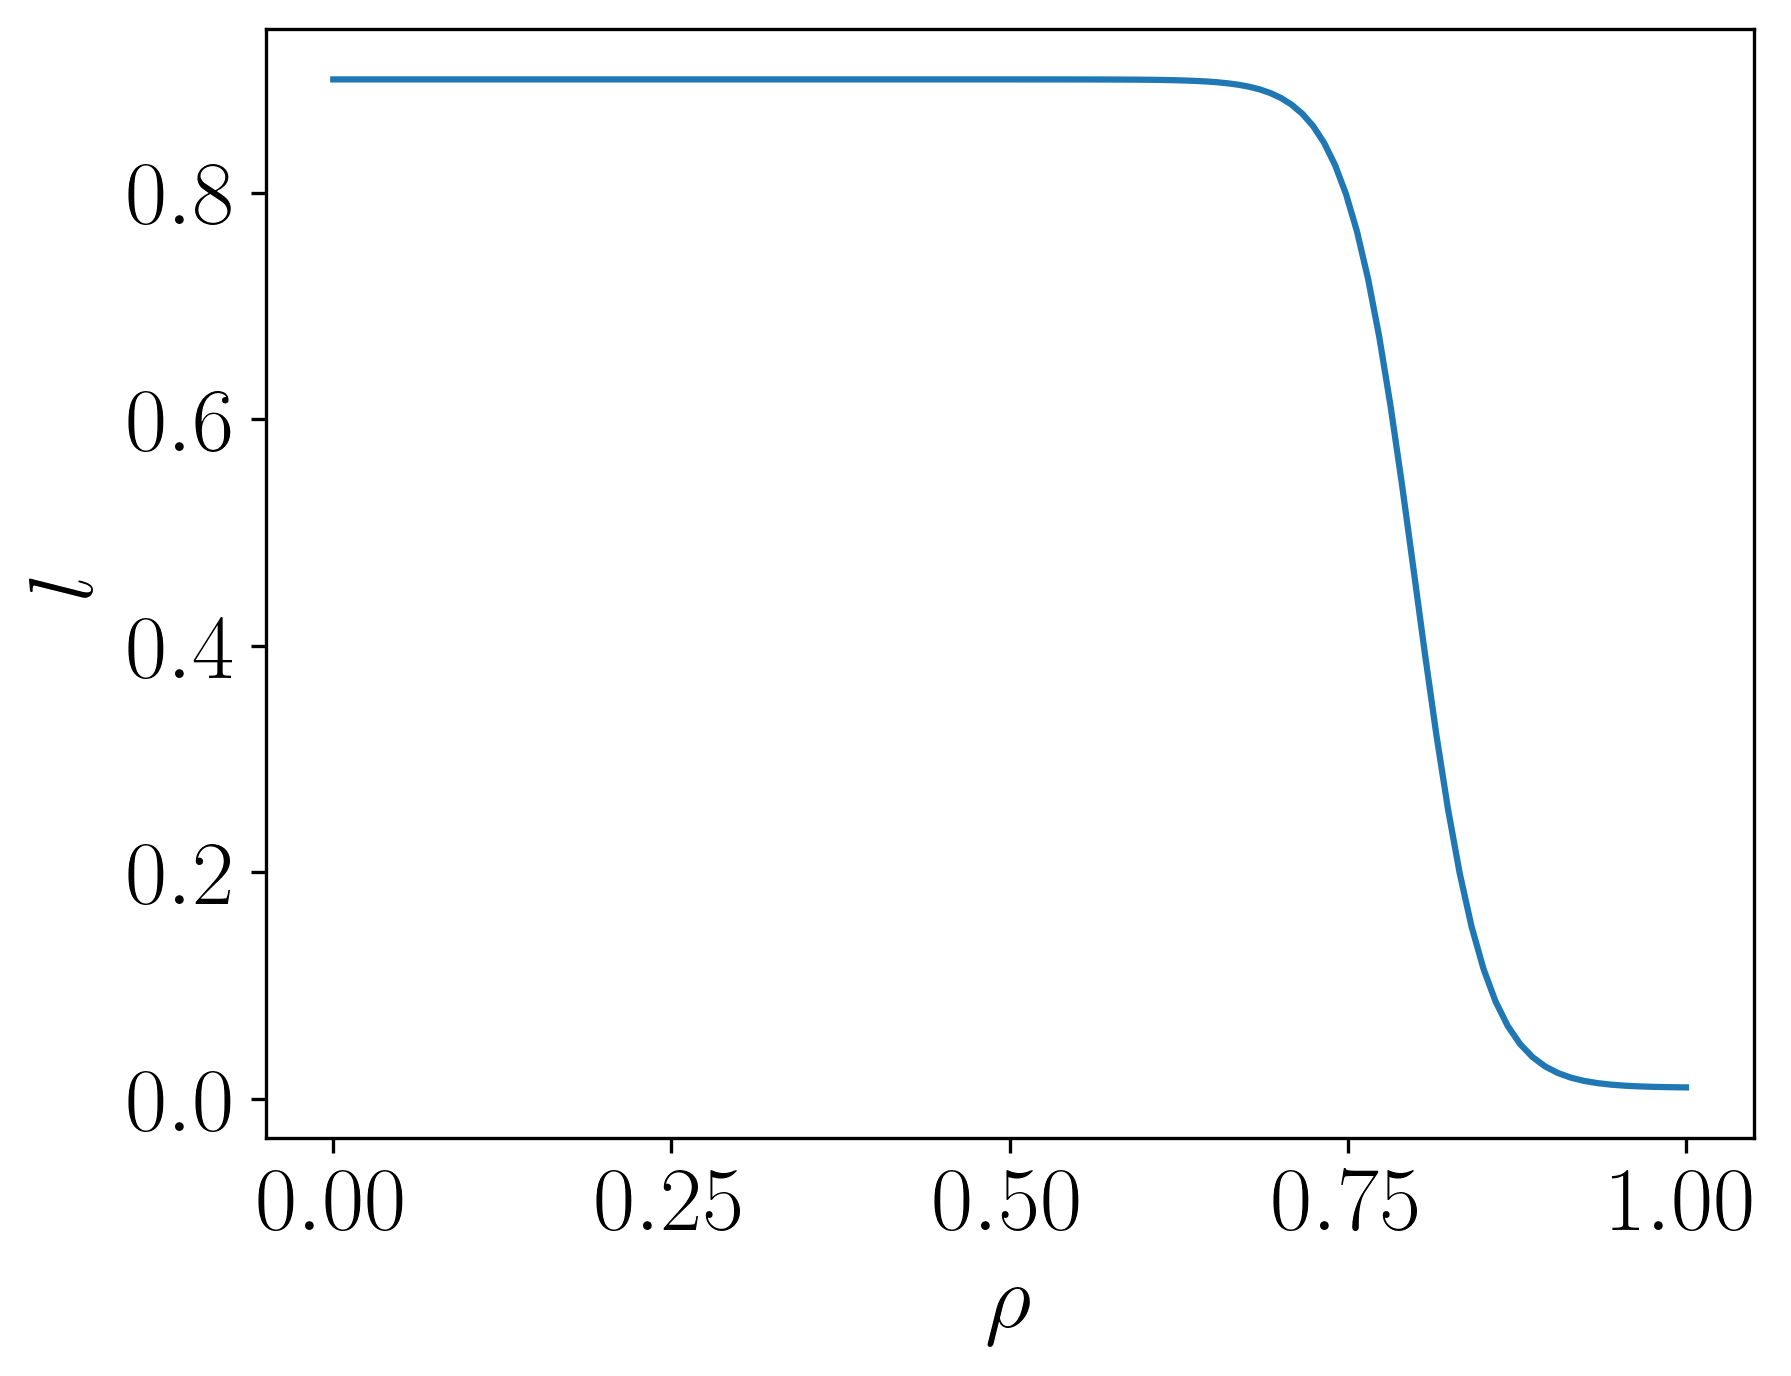
\includegraphics[width=10cm]{images/smoothstep.png}
  \caption{Hyperbolic tangent smooth step function for length scale, equation \ref{eq:smoothstep}. Used to capture the drop at the edge of H-mode plasmas \cite{chilenski}.}
  \label{fig:smoothstep}
\end{figure}

Traditionally prior information should be included in the prior distribution. However, in practice this often makes the required inversion of the priors covariance matrix difficult or impossible. This is either due to limited computational precision or because the covariance matrix becomes non-positive definate. The inversion is required because the closed form expressions for $\vec{\mu}_{post}$ and $\Sigma_{post}$ involve inversions of both the likelihood and prior covariance matrices. Although the likelihood covariance matrix $\Sigma_{li}$ is diagonal and so is certainly positive definite and inversion does not suffer from precision errors. This is not true for the priors covariance matrix $K$. It is difficult to define a prior covariance matrix that includes all the prior information, remains non-positive definite and does not suffer from precision errors. For these reasons, it is often more convenient to place prior information into the likelihood in the form of artificial observations. This method was also adopted by Chilenski \cite{chilenski}. The density is known to be close to 0 at the plasma boundary, ($\rho=1$). It is also known that the density profile is smooth and symmetric meaning the gradient of the profile on the magnetic axis must be close to 0. This information can be included in the data, $\vec{d}$, with an artificial experimental error determining the strength of the information included in $\vec{\epsilon}$. Other parts of the method need to be altered to accommodate the new information. The vector to be infered $\vec{a}$ is not only $\vec{n_e}$ but also includes $n_e(\rho=1)$ and $n_e'(\rho=0)$ concatenated onto the end. This allows the response matrix alteration to be simple,

\begin{equation}
  R^{alt} = 
\begin{bmatrix}
 R_{m\times n} &   O_{m\times2} \\
 O_{2\times n} &   I_{2\times 2} \\
\end{bmatrix}
=
\begin{bmatrix}
 &       &    & 0         & 0\\
  &   R_{m\times n}    &    &  \vdots  & \vdots\\
  &       &    & 0        & 0\\
0 & \cdots & 0  & 1        & 0 \\
0 & \cdots & 0  & 0        & 1
\end{bmatrix},
  \label{eq:Ralt}
\end{equation}

\noindent where $n$ is the number of unknown electron density values in $\vec n_e$ and $m$ is the number of interferometry lasers. The prior covariance matrix must also be altered. The covariance between a gradient and non-gradient data point is simply the differential of the covariance over the gradient data point. For two gradient data points, it is a differential over each point.

\begin{equation}
  K'_{ij} = k'(\rho_i, \rho_j) = \frac{\partial k'(\rho'_i, \rho_j)}{\partial \rho'_i} \, \cite{chilenski},
\end{equation}

\begin{equation}
  K''_{ij} = k''(\rho'_i, \rho'_j) = \frac{\partial k''(\rho'_i, \rho'_j)}{\partial \rho'_i \partial \rho'_j} \, \cite{chilenski}.
\end{equation}

\noindent In this notation $\rho'$ indicates the position of a gradient data point. The alternate kernel is then,

\begin{equation}
  K^{alt} = 
    \begin{bmatrix}
      K & K'\\
      K'^{\top} & K''
    \end{bmatrix}.
\end{equation}

The necessary adaptations to our defined Bayesian regression method to accommodate interferometry data have been described. For reference, the various final distributions and expressions after the adaptations are fully shown in appendix \ref{append:distexpres}.

\section{Chapter Summary}

The electron density profile is important as it plays a key role in determining the energy confinement time and informing real time control systems. With the assumption of magnetic flux surfaces, one can express it as a 1D profile. \gls{nice} is an equilibrium reconstruction code that also infers the electron density profile that can be used as a comparison in this thesis. Bayesian inference with multivariate Gaussians describing the various distributions can be applied to interferometry data to infer the electron density profile. A non-stationary kernel can be used to allow the inference to have a model complexity that varies with $\rho$. Hyperparameters can be tuned by minimising the negative log marginal likelihood. Alternatively, the hyperparameters can be marginalised. Prior information can be easily included in the likelihood with artificial observations. In the results section, these methods will be deployed on synthetic data. The inference performance can be determined by how closely it fits the ground truth profile. They will also be deployed on real \gls{west} data and the results will be compared to that obtained by \gls{nice}.

% \begin{figure}
%   \centering
%   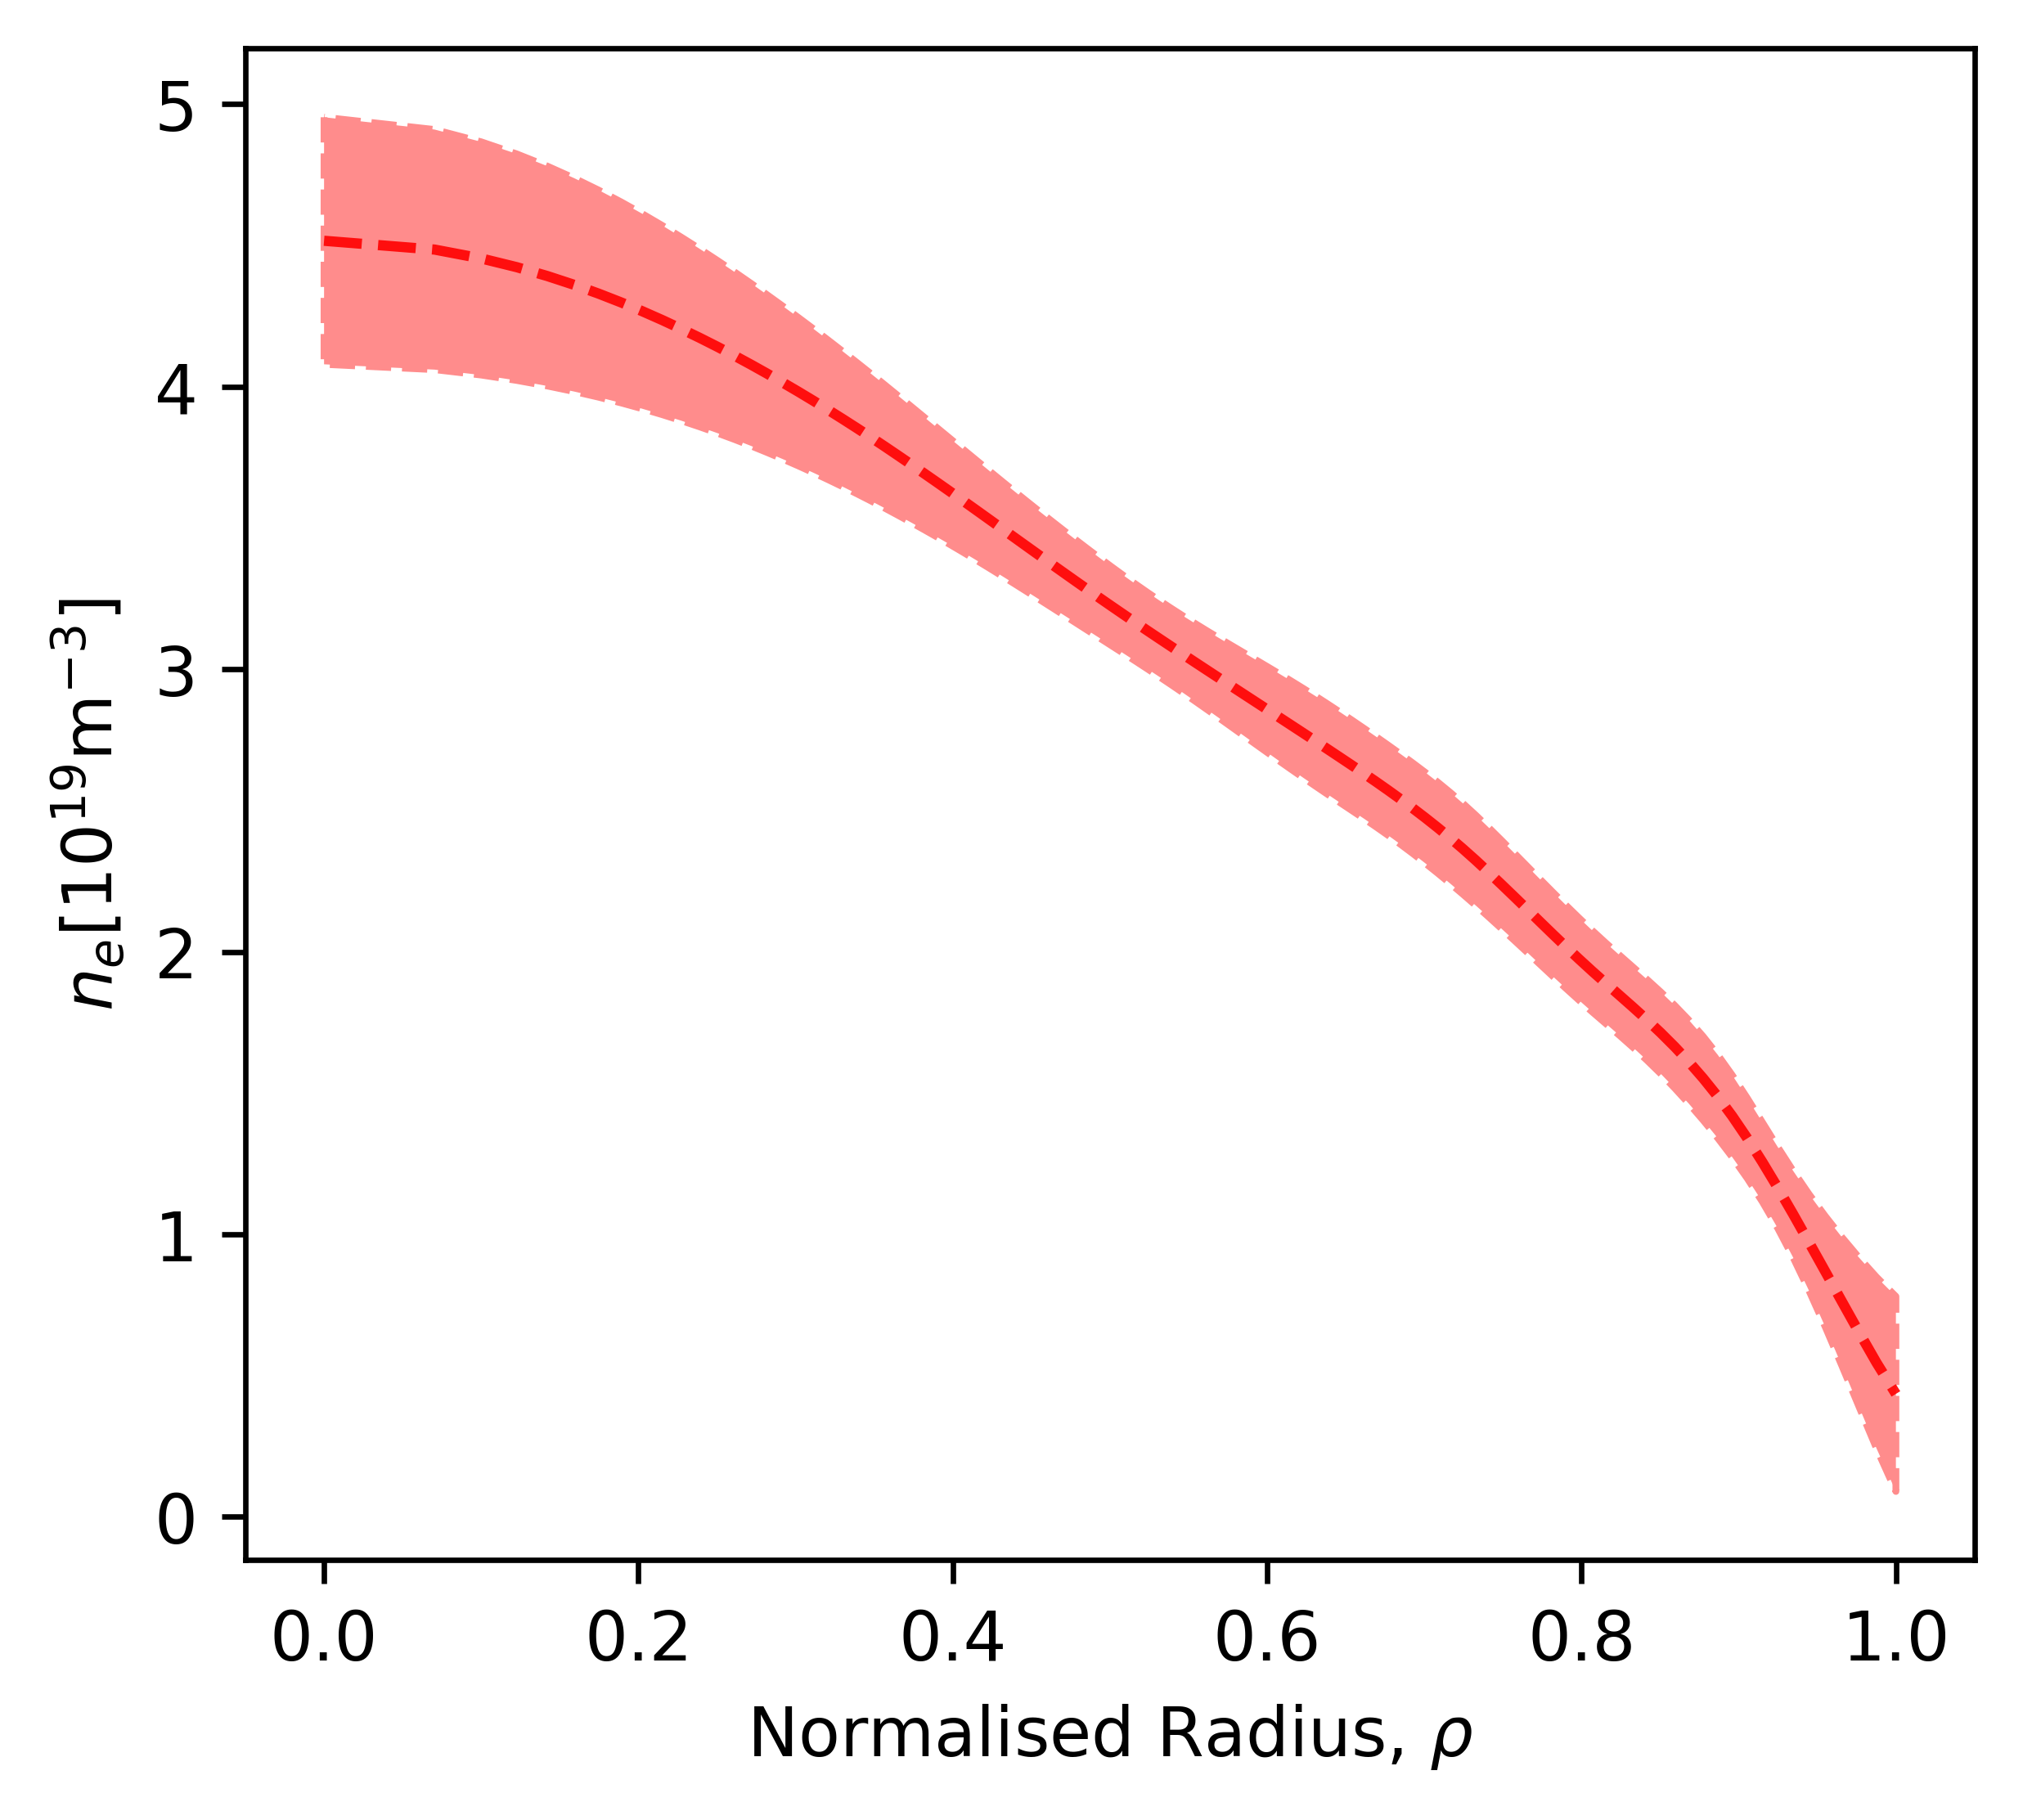
\includegraphics[width=\columnwidth]{images/niceExample.png}
%   \hskip 1mm
%   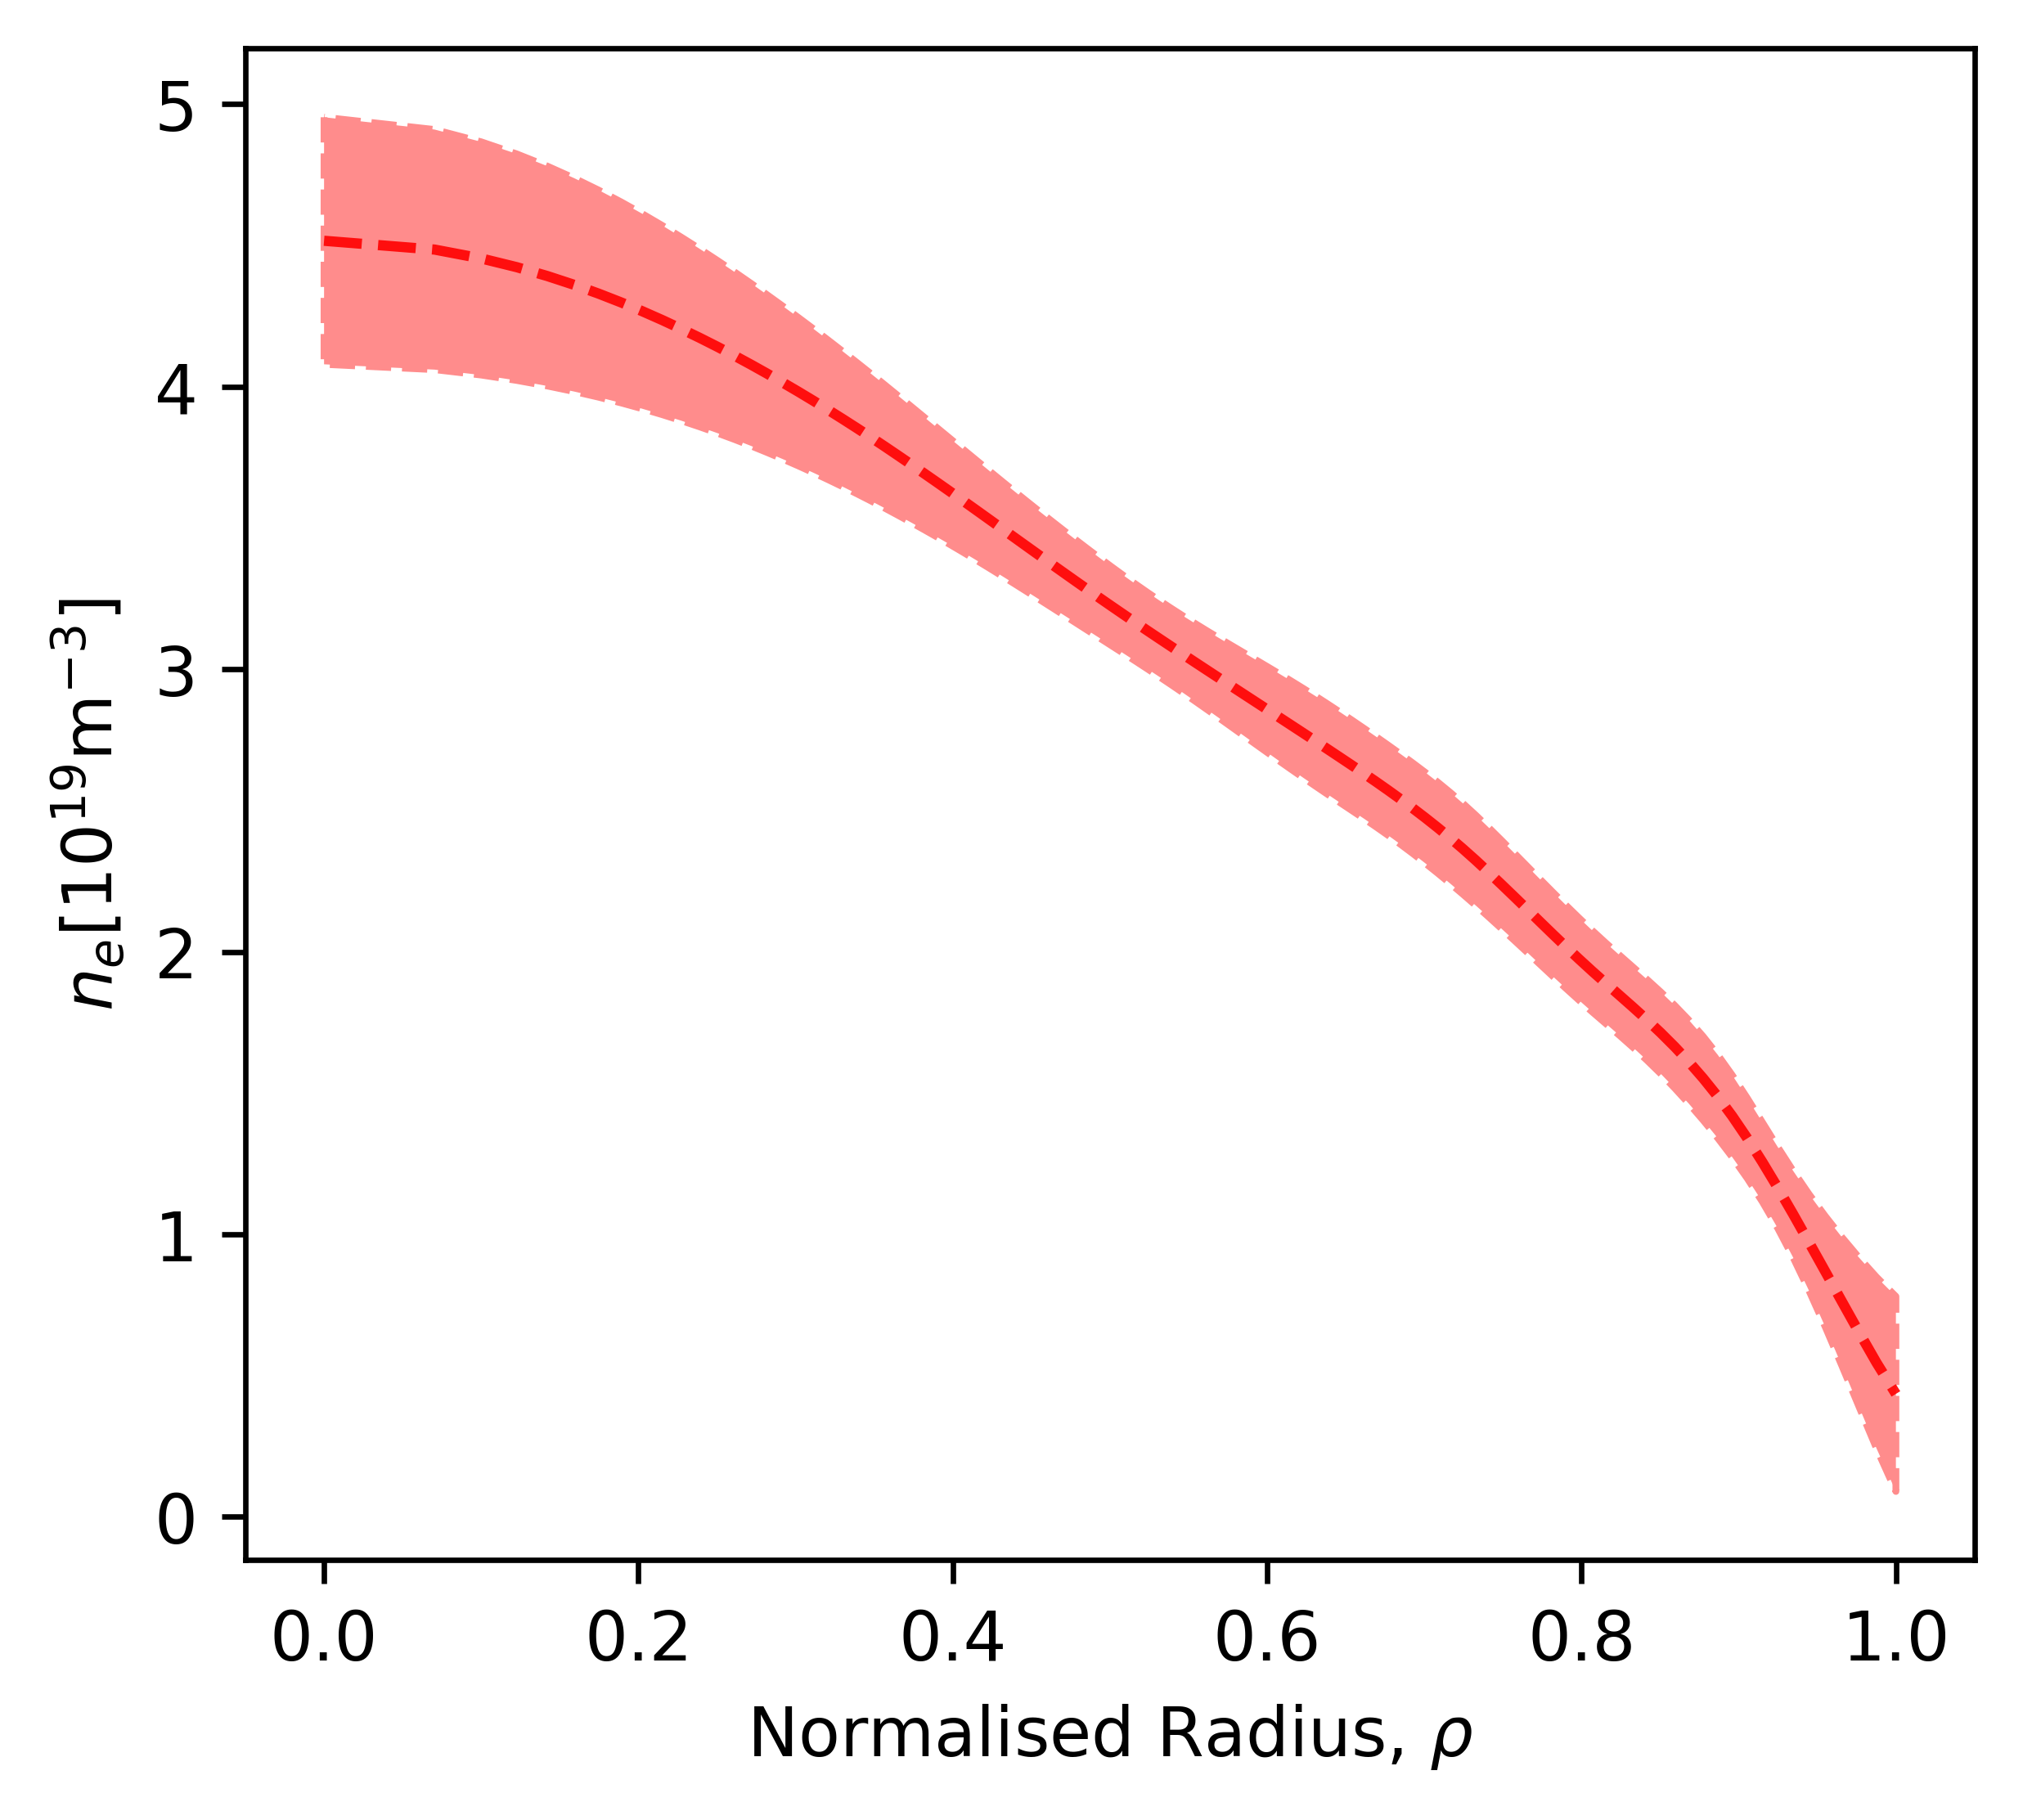
\includegraphics[width=\columnwidth]{images/niceExample.png}
%   \hskip 1mm
%   \vspace{-1cm}
%   \caption{Predictions on completely sampled space.}
%   \label{fig:flowe_grid}
% \end{figure}

% \label{sec:intpol}
% \section{Interfero-polarimetry}


% \begin{itemize}
%     \item Some basic background theory of a tokamak as a fusion device. Including the schematics of the magnetics and different systems present. Including the magnetic flux surfaces and what they are, assumptions made. What is $\rho$? Also highlights a little why the plasma density profile is important. 
%     \item Explain the theory of how NICE did their inference to some degree. ***
%     \item Bayes' theorem for inference problems, each distribution involved and why the marginal likelihood is useful. ***
%     \item Explian how a multivariate Gaussian can model a curve. ***
%     \item Explain Gaussian Process Regression for a generic line fitting problem, including the various distributions constructed and how they are used in the closed form expressions. A little on marginal liklyhood again for parameter optimisation. Mention briefly the alterations to this algorithm that will be made to allow it to be used for interferometry including the response function change, and virtual observations.
%     \item Explain Interferometry and a little on polarimetry, show west laser geometry
%     \item Explain the magnetic flux surfaces again a little and how this allows us to make the electron density profile 1D again.
%     \item Explain the forward model and how it is computed with the response matrix.
%     \item Explain how the prior edge and core information can be added and the complications of inserting it into the prior.
%     \item Explain why a non-stationary kernel (smooth step) might be beneficial 
%     \item summarise the chapter and explain how it ties into the methodology
% \end{itemize}

\chapter{Methodology and Results}

THE TEXTHEIGHT IS \the\textheight
THE TEXt width IS \the\textwidth

The previous section outlined the procedure for using Bayesian inference to solve a simple regression problem. It then expanded the concept to allowing for regression where the data is not in the same space as the inference result. The two spaces being connected by a forward model or responce matrix. This is exactly what is required as interferometry data is not in the same space as the profile to be inferred. Two main methods for dealing with the hyperparameters were also outlined. They are \gls{map} and marginalisation. Results will be presented for both sections. Both allow for hyperpriors to be included. A uniform prior is used for all hyperparameters and the bounds were selected by carefully observing how the parameters affect the resulting inferrence and allowing generous amount of room for profile extreamities to exist. The amplitude is constrained between $0$ and $100$ and is on the same scale as the electron density $\cdot 10^{20}$. Each length scale is bounded between 0 and 3 and is on the same scale as the normalised radius. This includes the non static kernel varients hyperbolic tangent length scale and cubic spline length scale. 5 knots were used for the cubic spline. To reduce the dimensionality of the problem they were evenly spaced across the normalised radius. Each interferometry channel is assumed to have the same experimental error and it is bounded between $0.03$ and $0.3\, \cdot10^{-19}m^2$. WEST reports a no plasma noise in the order of $0.03 \cdot10^{-19}m^2$. The hyperparameter \gls{map} is found by minimising the loss function based on the marginal likelihood, see equation \ref{eq:loss}. When any trialed parameters exceed their prior bounds the loss returns infinity (or a very high number). SciPy minimise and PyTorch SGD are both gradient based methods that were trialed and achieved similar results. In order to precisely measure the accuracy of the inferences a known ground truth profile is required. The metric used is mean square error and is included on each graph as `mse'. There are a few main profile types of interest to the scientific community. L mode or low confinement profiles are typically parabolic like in shape and are the bread an butter of tokamak operation. It is the easiest profile to achieve and is often a stepping stone to achiving other profiles within a plasma shot. This is the main profile used within the \gls{west} tokamak. H mode or high confinement mode is achieved by increasing external heating power from sources such as neutral bean injection and electron cyclotron resonance heating. H mode profiles have a distinct sharp drop in density near the plasma boundary. H mode profiles are well known for largely increasing the energy confinement time of the plasma which is a cruicial factor for net positive energy production. Although they do introduce extra instabilites known as ELMS. Another interesting profile feature is known as peaking. The external heating elements can be tuned to target the core. The extra heat ionises more of the fuel and decreases electrion-ion recombination rates. This increases the electron density in the core and creates a peak or bell shape profile. This can be achieved with both L mode and H mode. Peaking is known to increase the stability and performance of the plasma. It helps reduce the impurities in the core that contribute to radiation loss. Versions of these profiles are shown in figure \ref{fig:groundtruth}. The interferomety data that would be measured given a profile as the ground truth is computed with the responce matrix. The responce matrix is created using real magnetic field lines inffered by \gls{nice}. A generously small Gaussian experimental error is added with a standard deviation of $3\cdot10^-17 \, m^2$. This is what \gls{west} reports as the no plasma noise of the interferometer. 


\begin{figure}[ht]
    \centering
    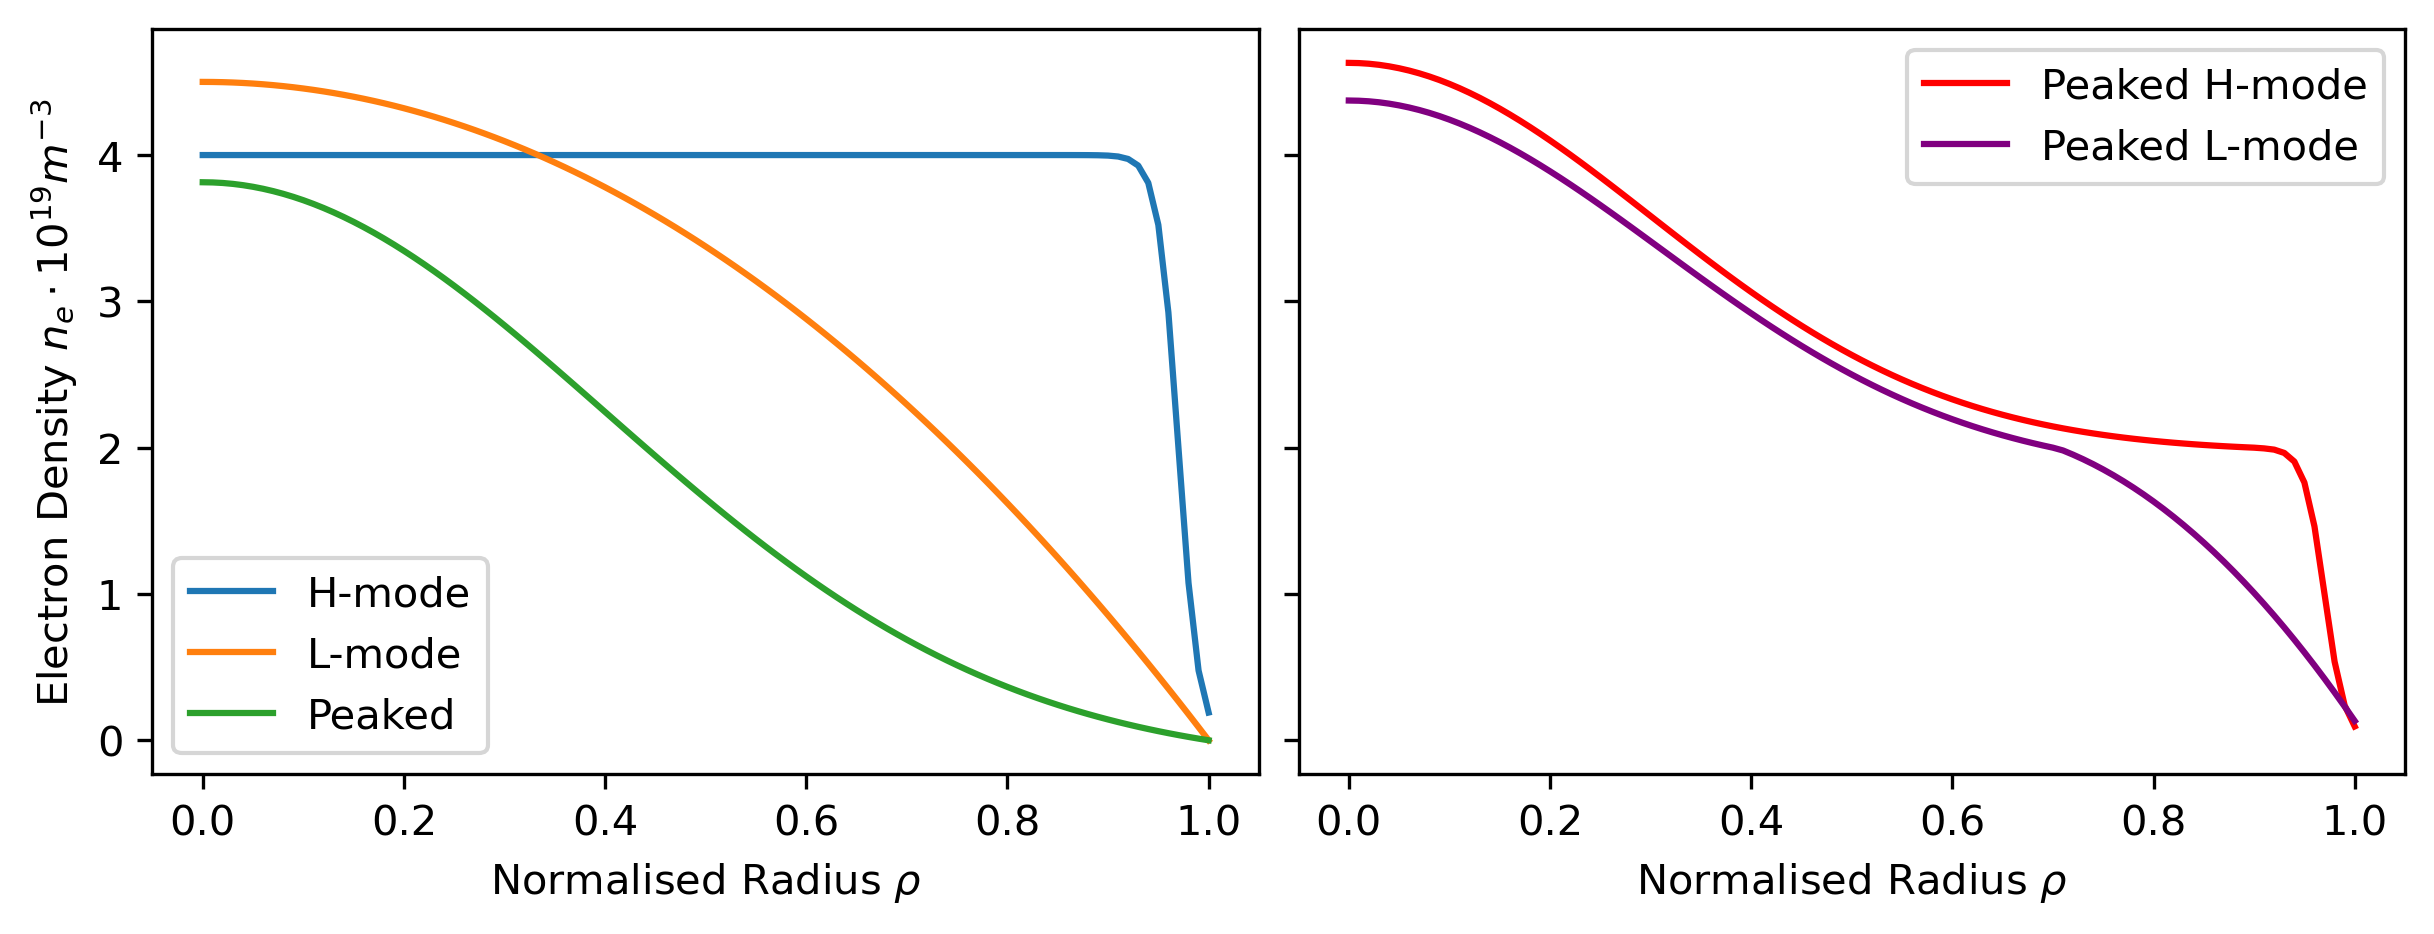
\includegraphics[width=\textwidth]{images/syntheticProfiles.png}
    \caption{Ground truth profiles used to generate synthetic interferometry data.}
    \label{fig:groundtruth}
\end{figure}

\begin{figure}[ht]
    \centering
    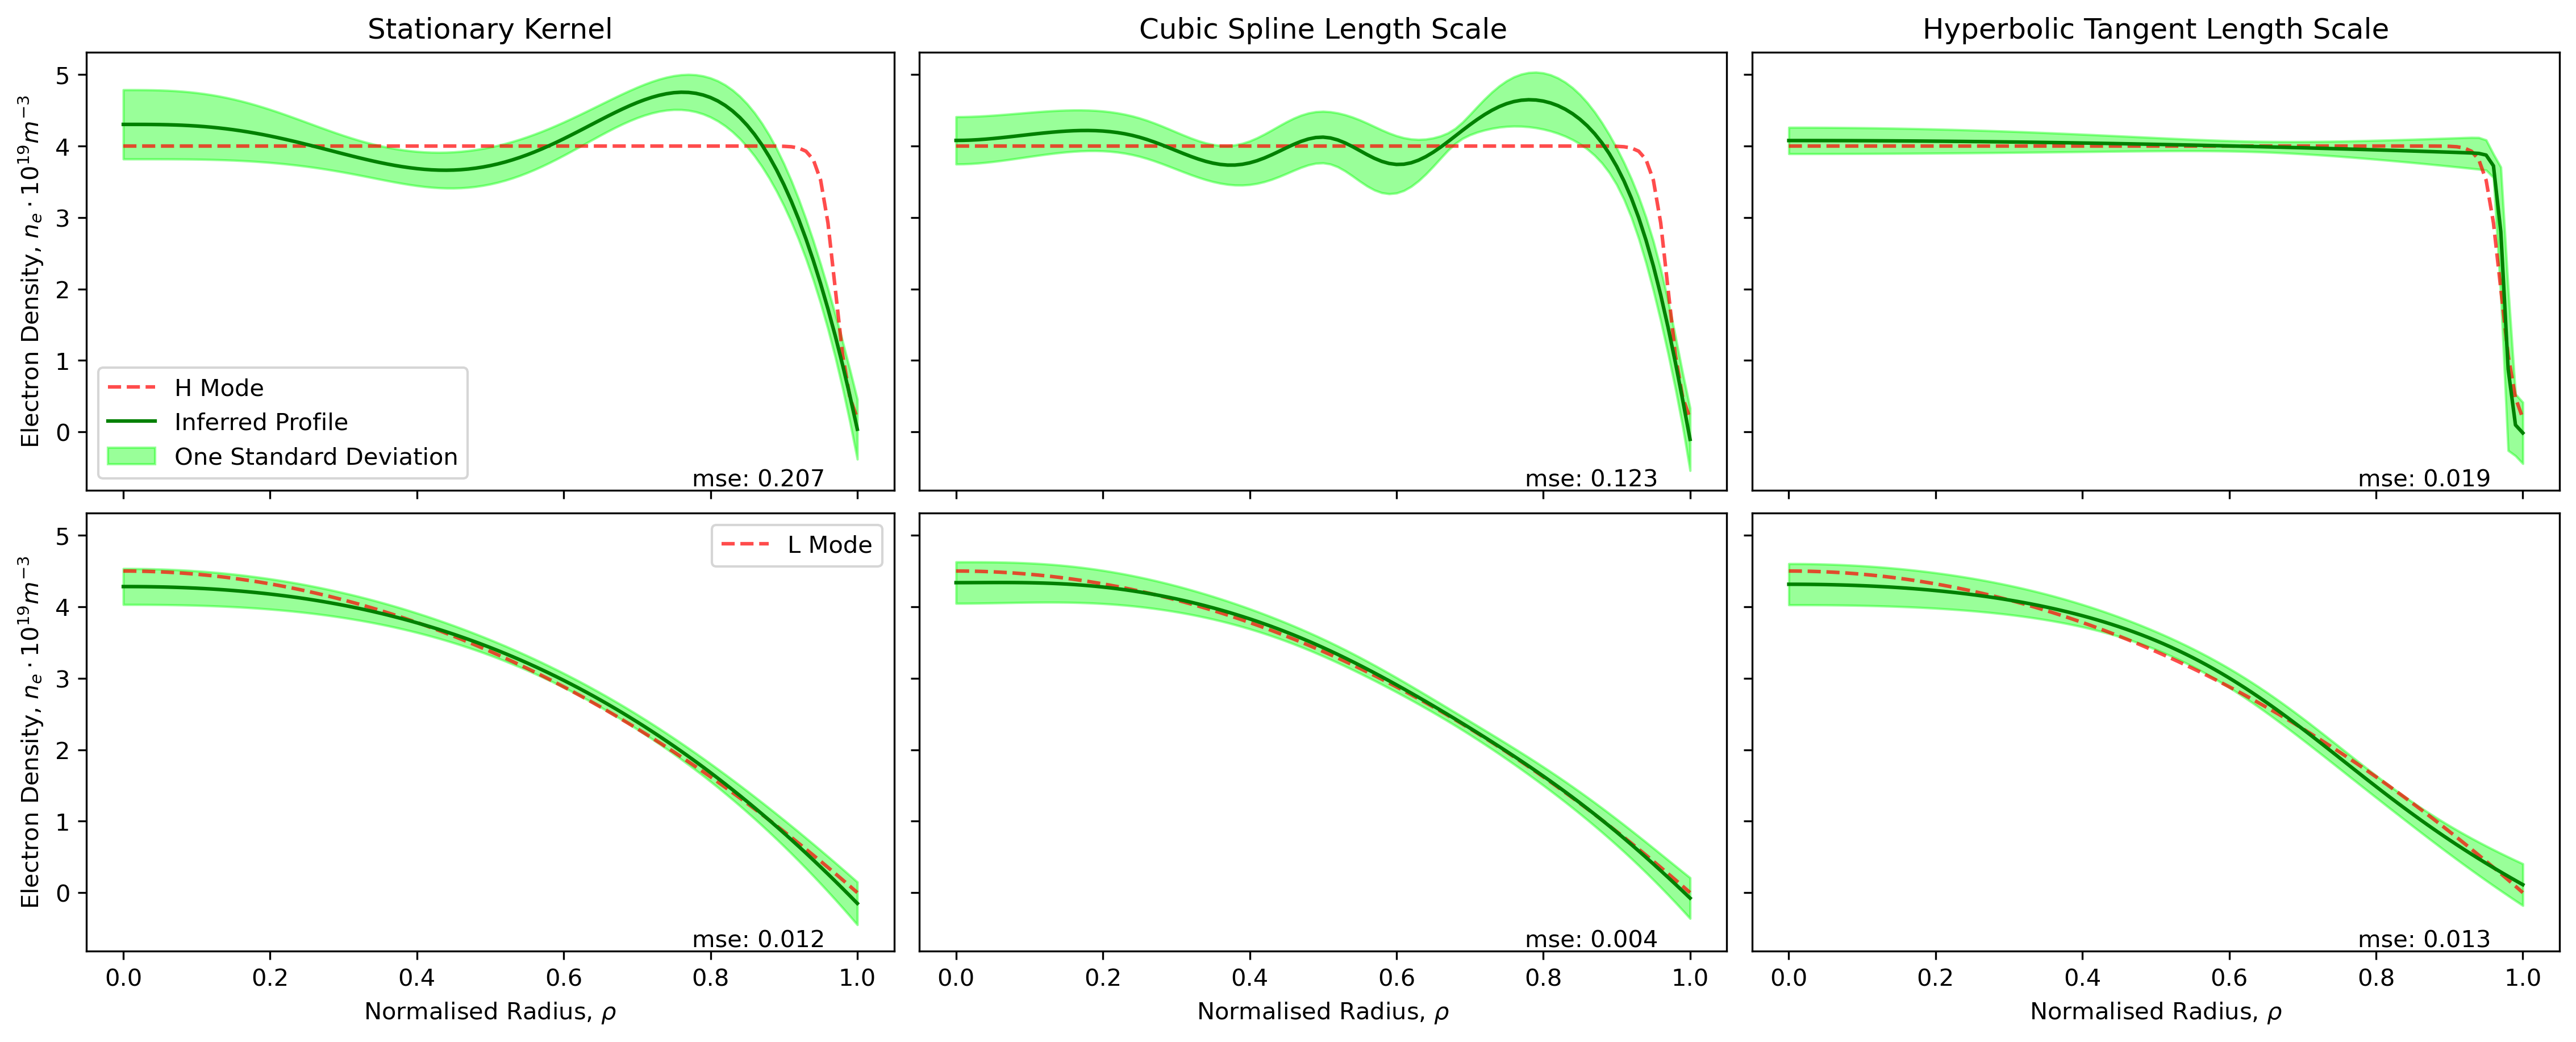
\includegraphics[width=500pt, angle=90]{images/Final/MAPsynthetic_final_hl.png}
    \caption{Electron density inference using the hyperparameter MAP method on synthetic interferometry data from H and L mode profiles.}
    \label{fig:mapsynthetic_hl}
\end{figure}

As expected the hyperbolic tangent was the most sucessfull at inferring the H mode profile, see figure \ref{fig:mapsynthetic_hl}. This is because the constant flat top requires a high length scale yet the sharp drop requires a low length scale. A low lengthscale reduces the correlation between neighbouring inferred electron densities which is required for the high gradient at the edge. It is impressive how equally accurate and precise the three kernels are at inferring the L mode profile.  

\begin{figure}[ht]
    \centering
    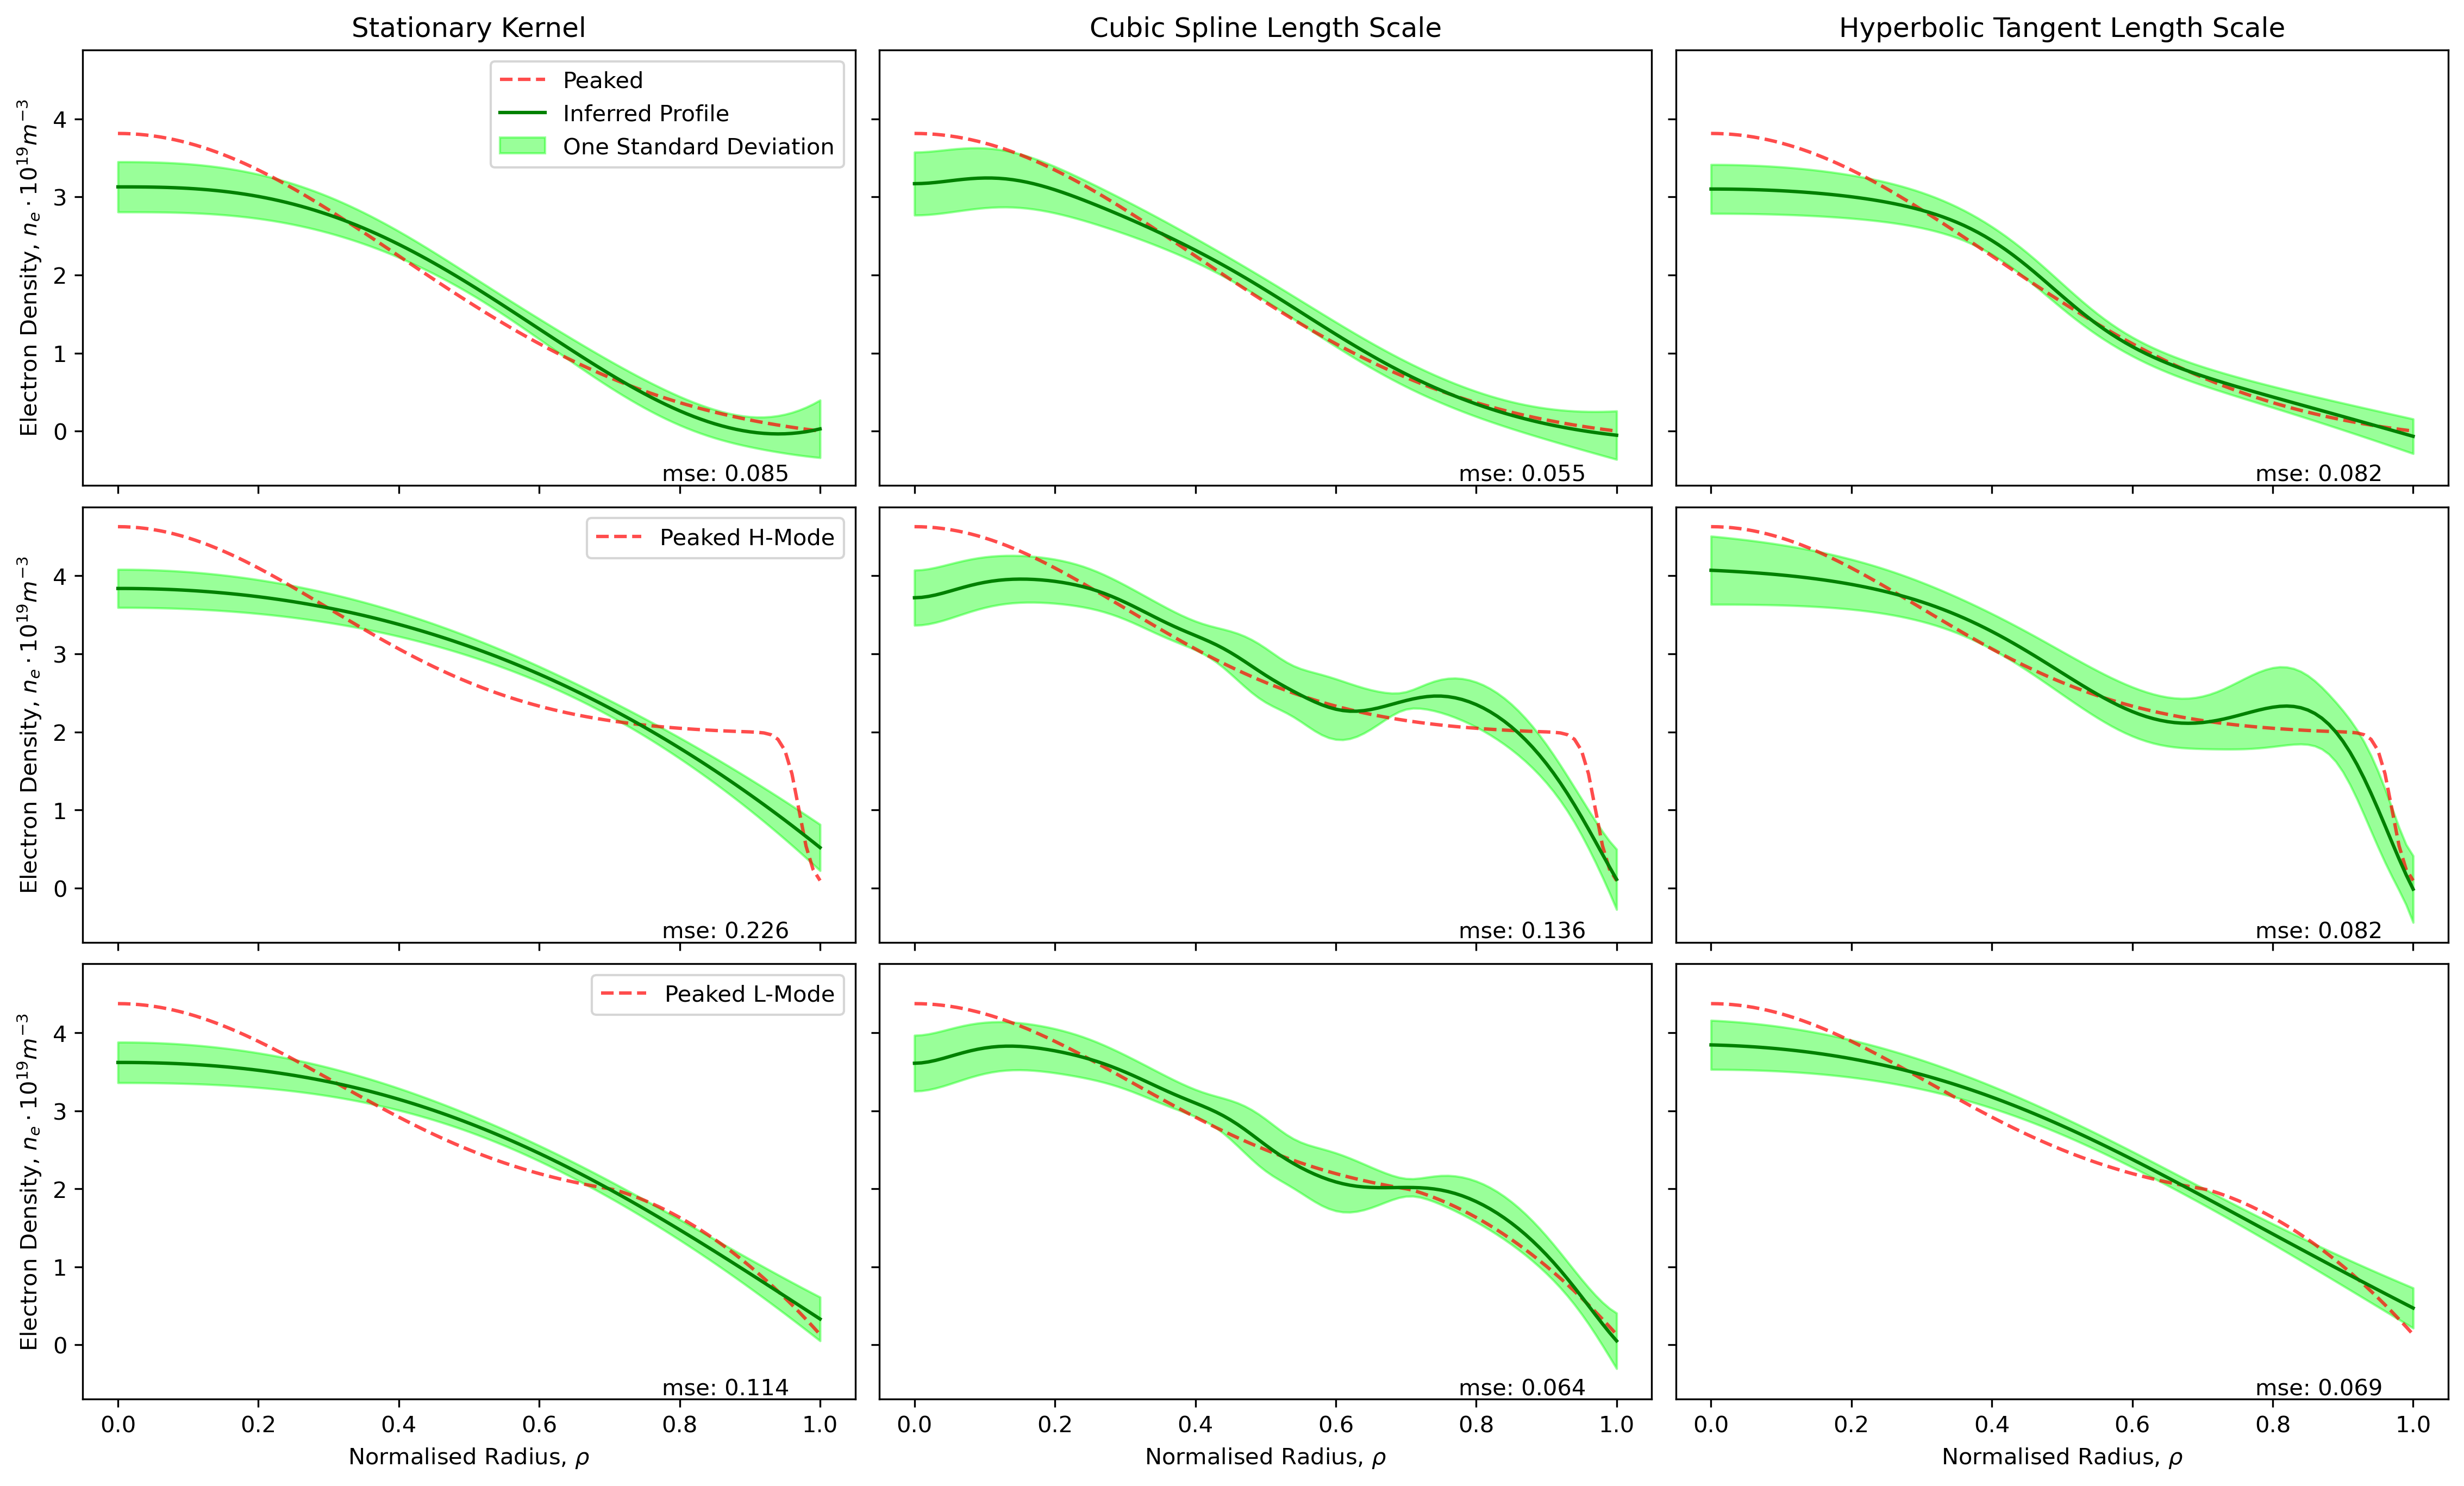
\includegraphics[width=500pt, angle=90]{images/Final/MAPsynthetic_final_p.png}
    \caption{Electron density inference using the hyperparameter MAP method on synthetic interferometry data for peaked profiles. The mean square error is shown as `mse'.}
    \label{fig:mapsynthetic_p}
\end{figure}

The static kernel performed poorly when faced with a more complex shape such as the peaked L and H mode profiles, see figure \ref{fig:mapsynthetic_p}. It appears close to parabolic and this is likely due to the length scale being inferred too large. The cubic spline length scale showcases its flexability, allowing it to find some of the profile features although this appears to come at a price of smoothness. The hyperbolic tangent was able to find the H mode edge but not as closely as it was in the pure H mode profile as the core lengthscale needed to be lower to allow for the curvy peak. It still outperformed the other kernels for the H mode peak. The hyperbolic tangent has the lowest average 'mean square error' over all the profiles at $0.053$. Cubic splines is second with $0.076$ and the stationary kernel performed the worst with $0.129$.

Marginalising the hyperparameters is an alternative approach that was introduced. This involves using \gls{mcmc} to sample from the hyperparameter posterior. This thesis uses the emcee python package which is based on the affine-invariant ensemble sampler proposed by Goodman and Weare \cite{emceeGoodman}. This method uses many `walkers' that explore the parameter space in parallel, and update their positions by placing the position of another walker into the proposal function. The advantage of this method is that it is invariant to affine transformations of the parameter space. Since a unique posterior distribution can be analytically computed from the hyperparameters, sampling hyperparameters is equilivant to sampling many posterior distributions. Since each posterior is a multivariate Gaussian sampling from them is trivial and this thesis uses the scipy stats multivariate Gaussian random variable sampler to perform the operation. One $\vec n_e$ sample is taken from each distribution. Overall this is equivalent to sampling from a posterior that is independent of the hyperparameters $P(\vec n_e | \vec d)$. To perform the \gls{mcmc} sampling the analytical expression for the predictive log marginal likelihood is used. The same prior bounds are enforced as in the \gls{map} method. 

To minimise autocorelation the emcee hyperparameters are tuned. For emcee the main hyperparameter is called `moves', which is their term for the proposal function. It is also possible to pass multiple moves and weights when sampling. Emcee will then randomly select a move in proportion to the weights. In theory, this should make the next sample more random and less correlated to the previous. Each move also has a single parameter. These can be trialled with smaller sample numbers in an attempt to minimise the autocorrelation. Optuna is a hyperparameter tuning framework for Python that proposes trials in an attempt to minimise the objective function. By default, it uses the tree-structured Parzen estimator algorithm which is also a Bayesian method. In this thesis four of the moves and their parameters are trialled with Optuna. Each trial was allowed to take 500 samples and 100 trials were made for the stationary kernel. The autocorrelation for each chain on each parameter is averaged. The lowest average autocorrelation time for each move is used to determine the parameter value of each move. It also determines the weights, allowing for the best performing move to be used more frequently. The computed weights are shown in figure \ref{fig:optuna} and this is also a probability distribution for their use when sampling.

\begin{figure}[ht]
    \centering
    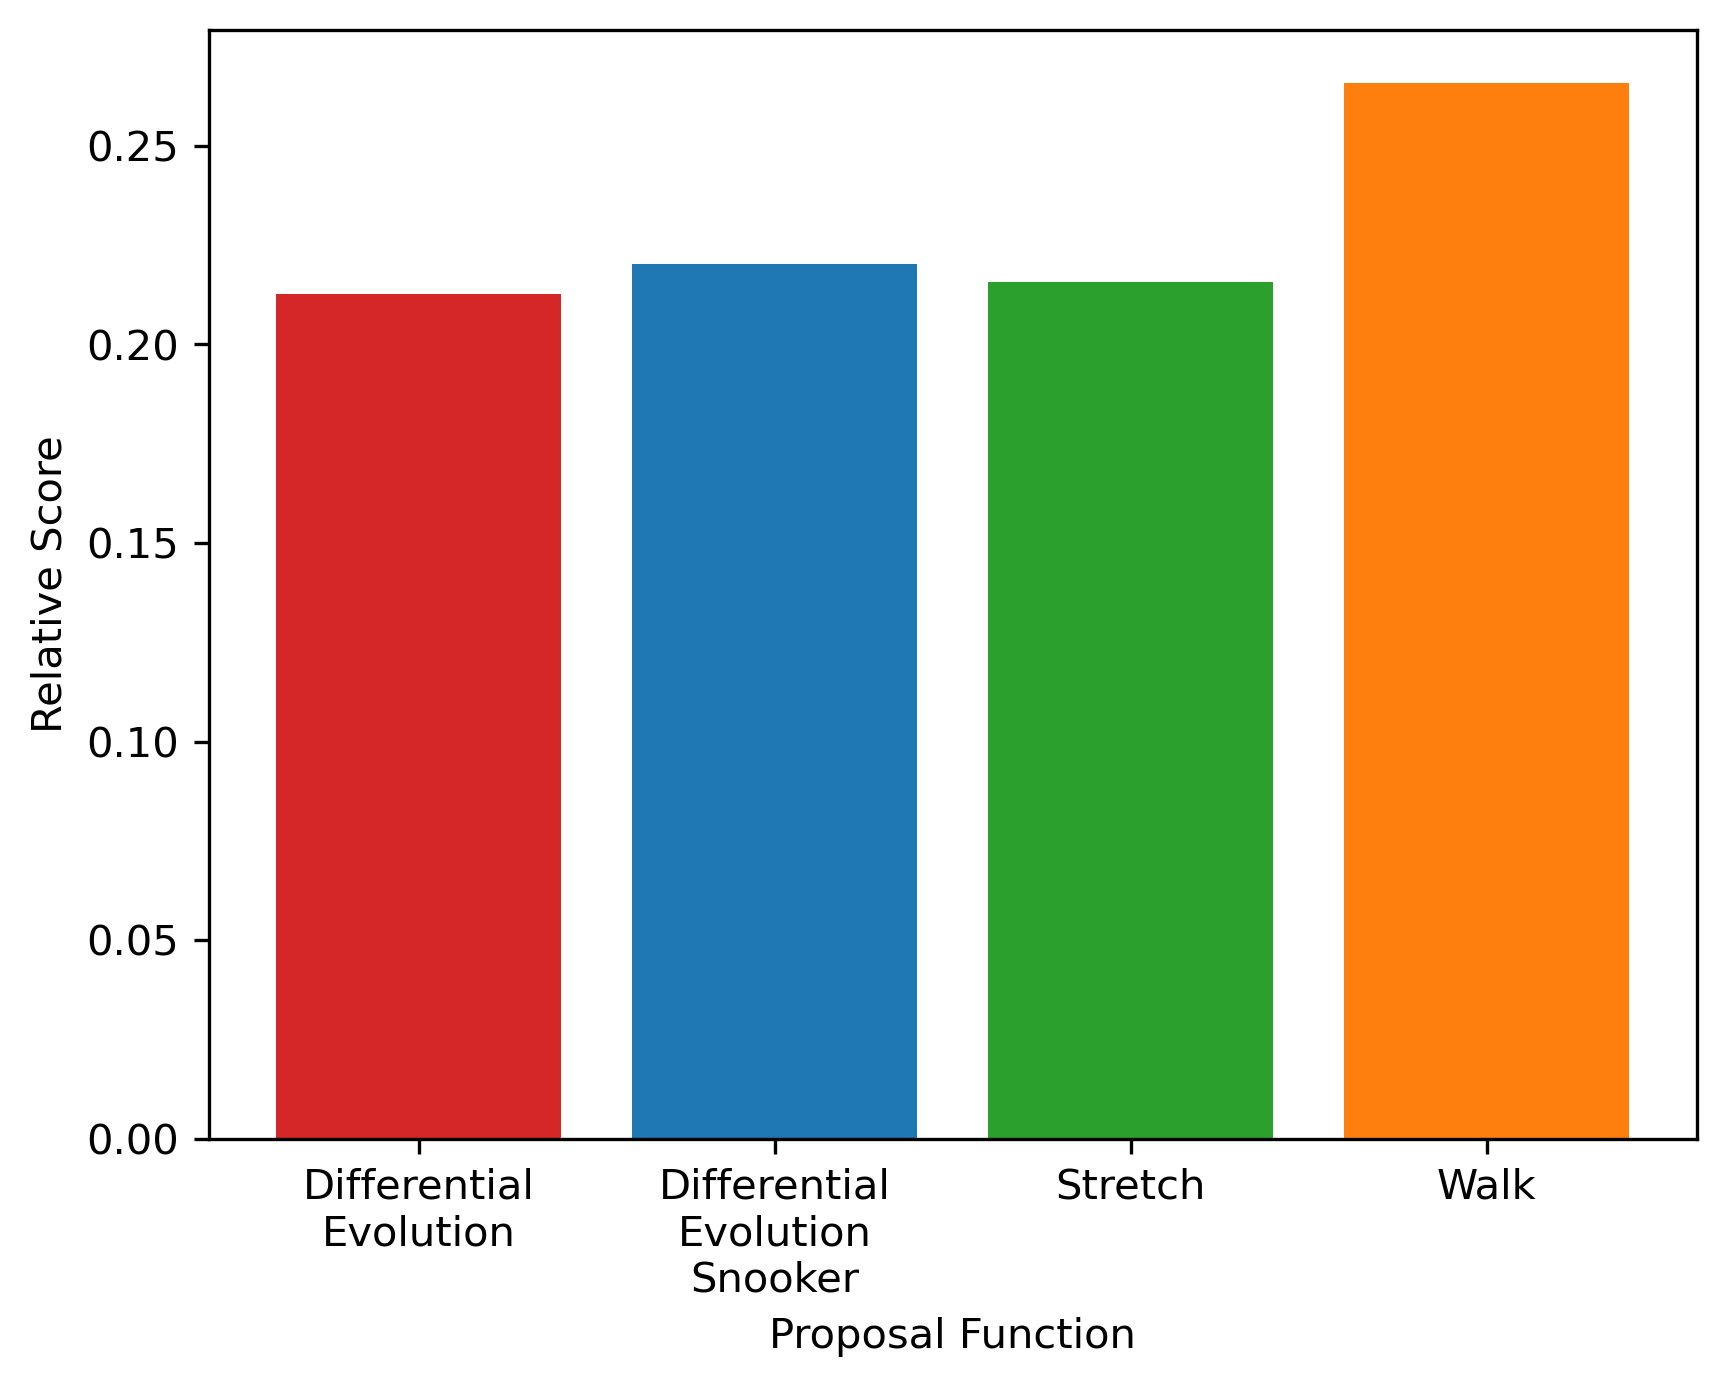
\includegraphics[width=300pt]{images/Final/optuna.png}
    \caption{The distrubution from which emcee proposal functions (moves) are selected based on perfomance in an Optuna evaluation.}
    \label{fig:optuna}
\end{figure}

They performed similarly well. Using the tuned moves combined with a burn in period of 1000 and thinning by degree 10 the autocorrlation was computed to be 23,6 for an example chain shown in figure \ref{fig:tracethin}. There still apears to be a significant amount of autocorrelation and this could affect the reliability of the results.  

\begin{figure}[ht]
    \centering
    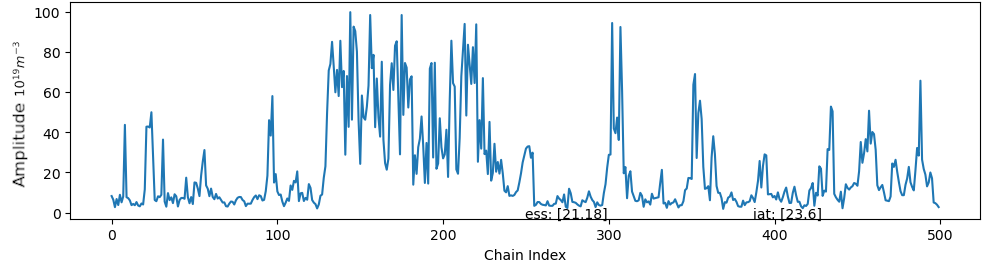
\includegraphics[width=\textwidth]{images/Final/TraceBurn1000_thin10.png}
    \caption{A trace plot showing the amplitude samples left after a burn of 1000 and thin of degree 10. The integrated autocorrelation time and effective sample size is shown as `iat' and `ess', respectivly.}
    \label{fig:tracethin}
\end{figure}

Tuning the emcee moves was not repeated for each kernel to save on computation. The same move weights are used to sample hyper parameters for the hyperbolic tangent and cubic spline non stationary kernels. 6000 samples with a burn of 1000 and thining of 10 is also used for these. The remaining 500 samples is used to compute 500 fixed parameter posteriors. One $\vec n_e$ is sampled per posterior with SciPy stats. Finally a mean and standard deviation is taken of these 500 $\vec n_e$ samples to obtain the final inferrence and uncertianty, see figures \ref{fig:fb_inference_hl} and \ref{fig:fb_inference_p}. Taking the mean and standard deviation allows for an easier comparison to the \gls{map} results. The distribution of $n_e$ at a point of normalised radius is plotted to ensure the mean is a suitable average to use, see figure \ref{fig:ne_dist}. The median and quantiles are also acceptable measures.

\begin{figure}[ht]
    \centering
    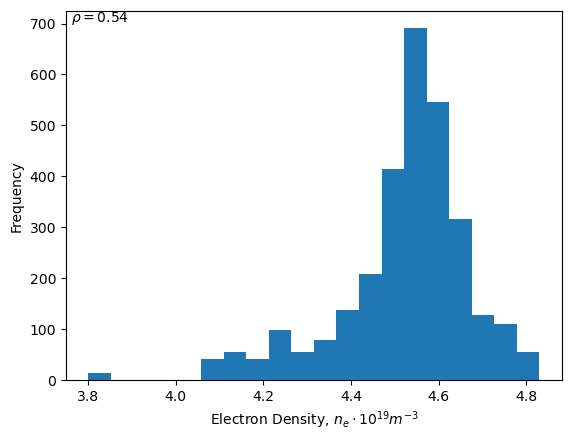
\includegraphics[width=300pt]{images/Final/sampled_ne_dist.png}
    \caption{An example distribution of $n_e$ for $\rho=0.54$ from the full Bayesian sampling method.}
    \label{fig:ne_dist}
\end{figure}

\begin{figure}[ht]
    \centering
    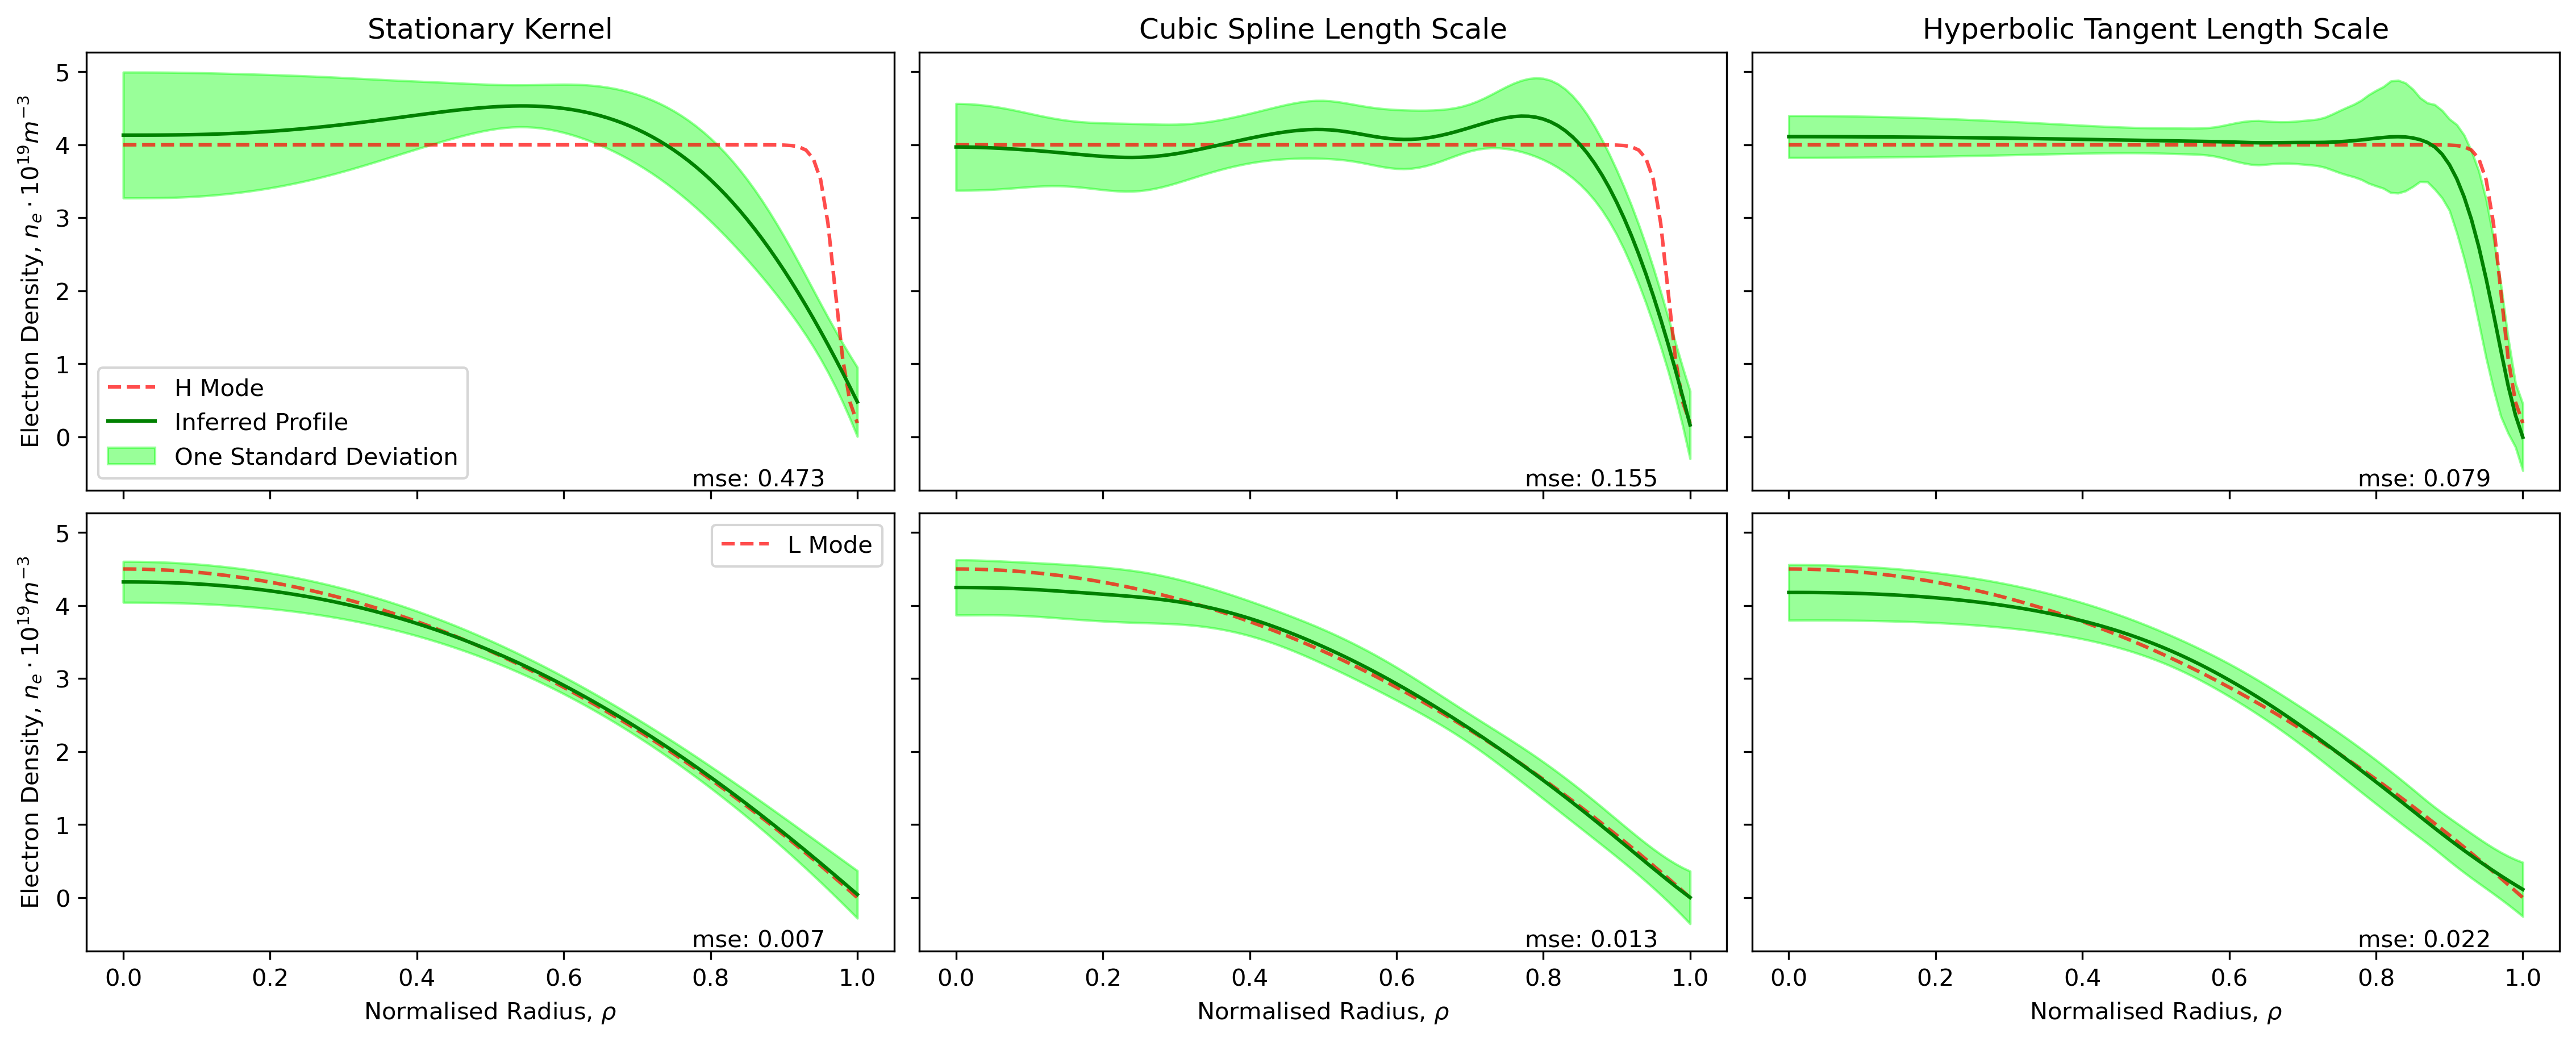
\includegraphics[width=500pt, angle=90]{images/Final/FB6000compute_noMAP_hl_burn1000_thin10.png}
    \caption{Electron density inference based on the full Bayesian method for synthetic interferometry data from H and L mode profiles. The mean square error is shown as `mse'.}
    \label{fig:fb_inference_hl}
\end{figure}


\begin{figure}[ht]
    \centering
    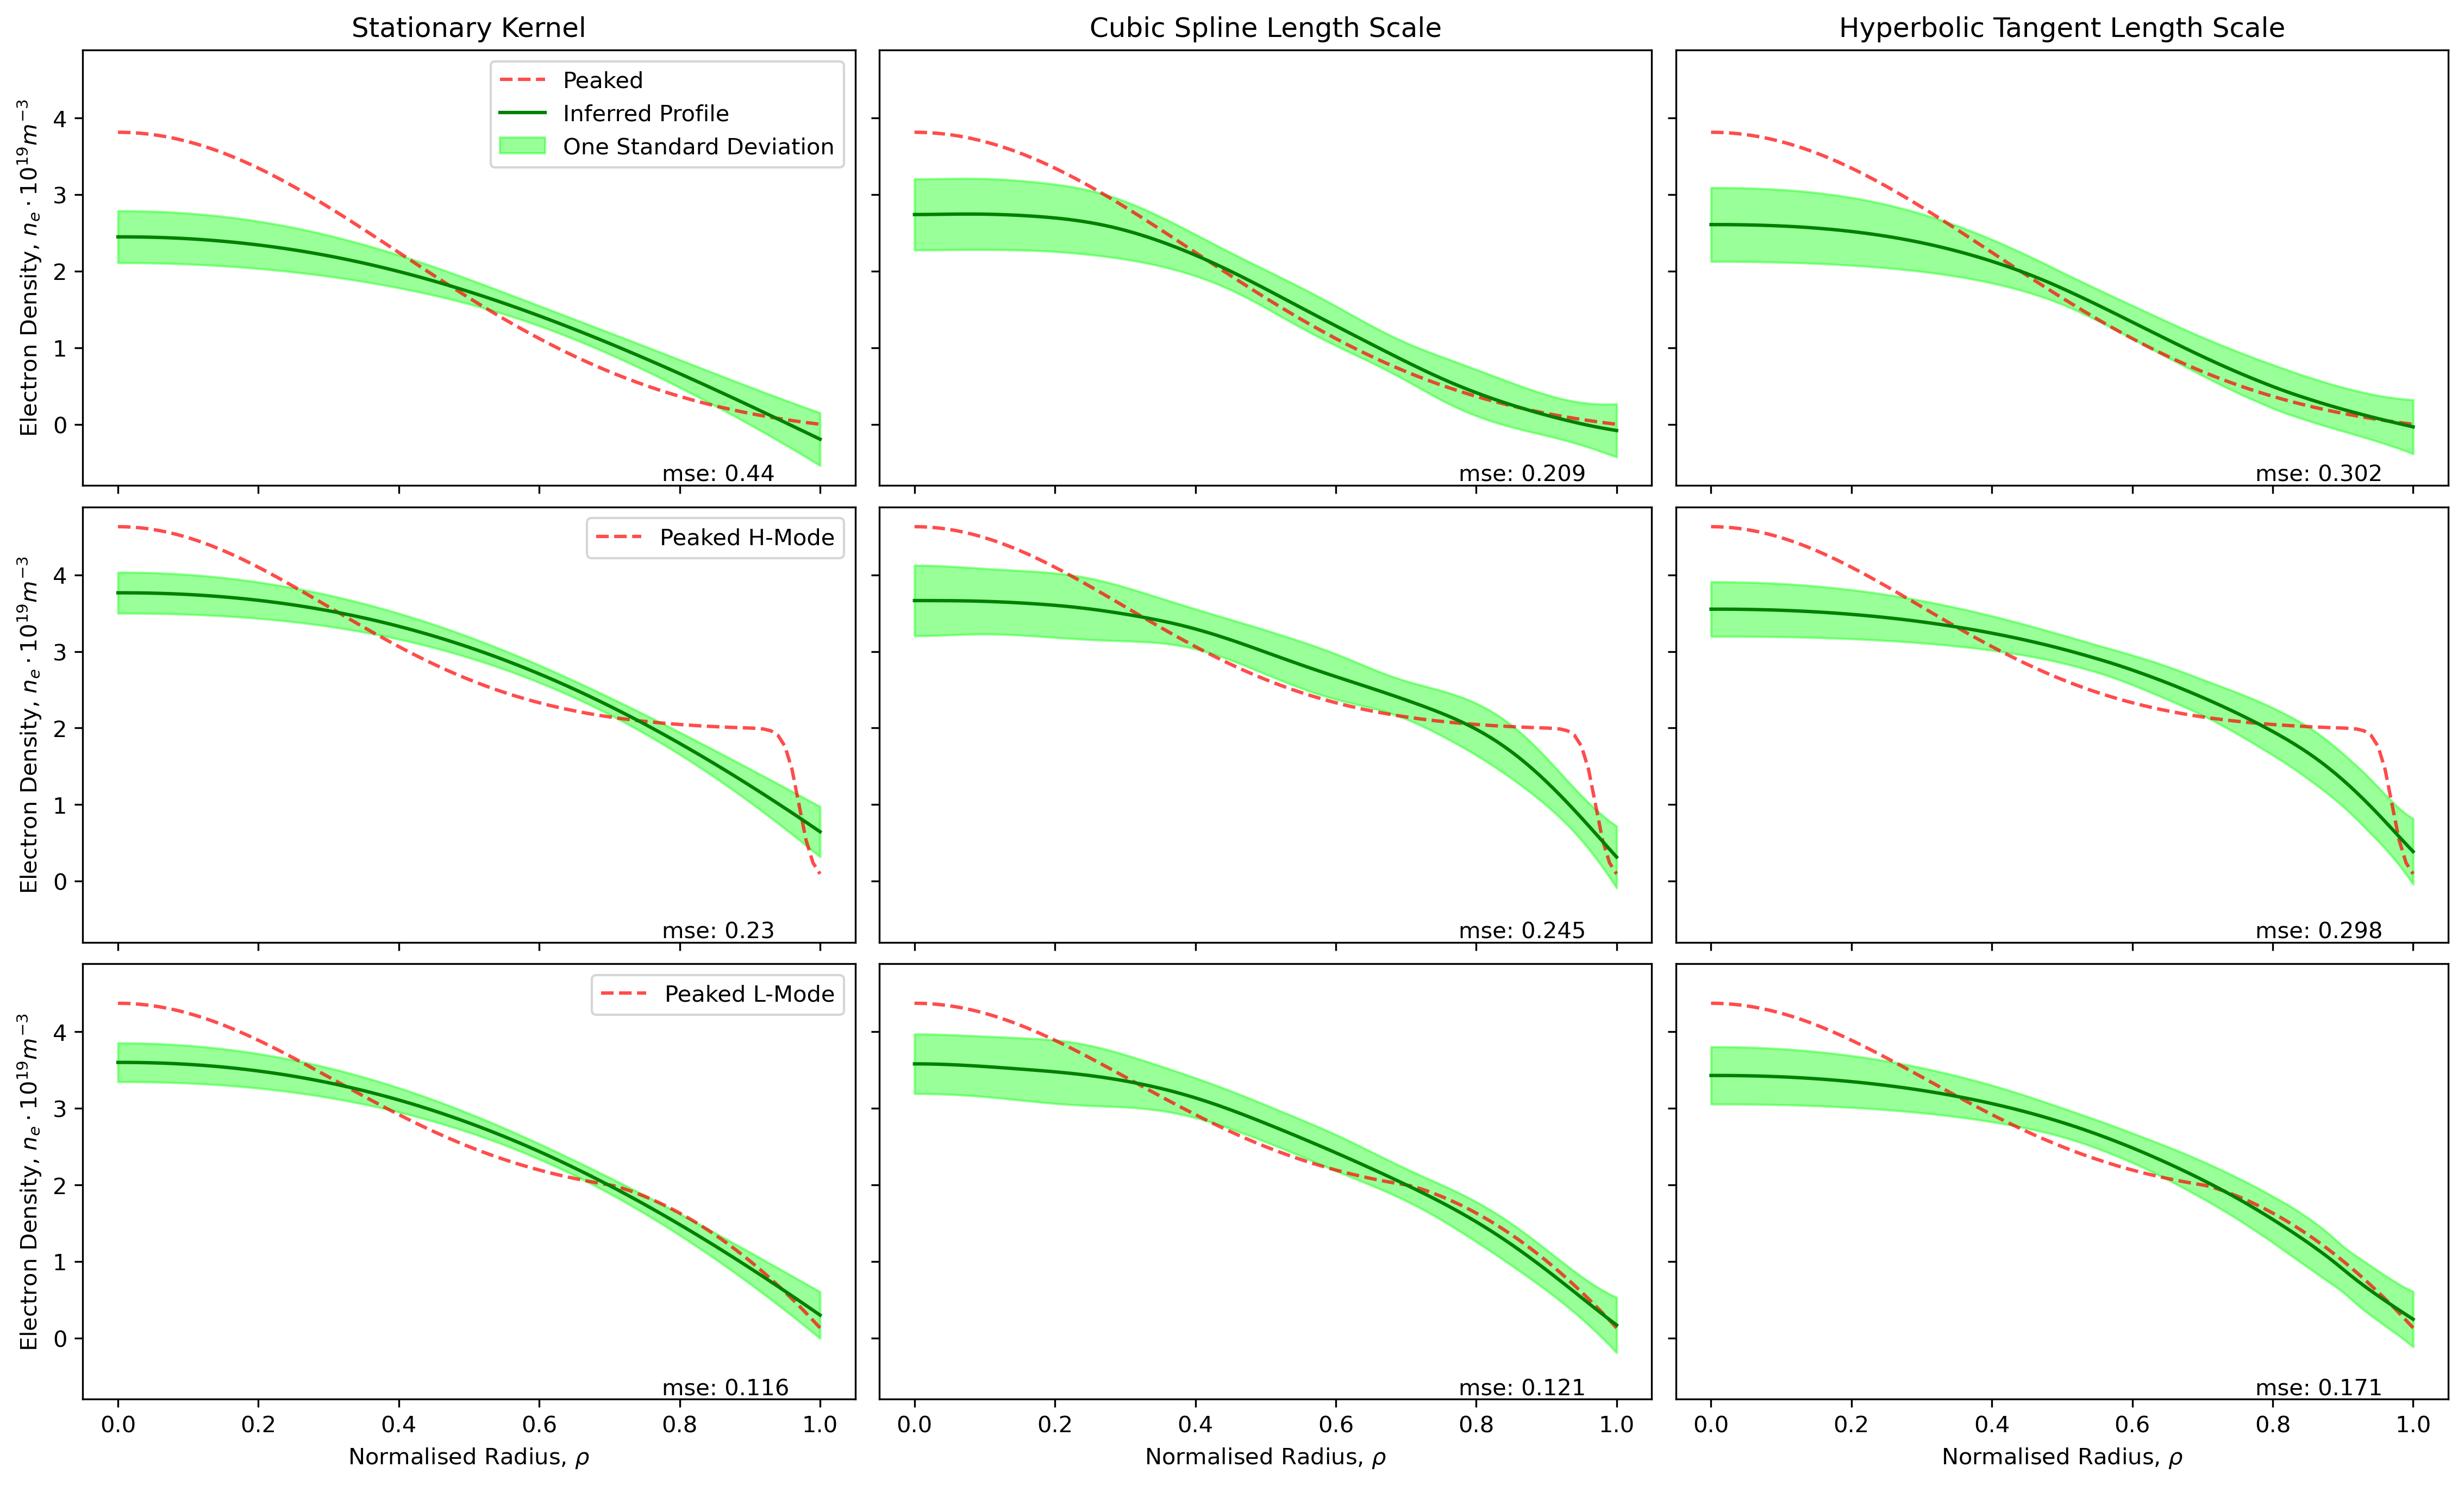
\includegraphics[width=500pt, angle=90]{images/Final/FB6000compute_noMAP_p_burn1000_thin10.png}
    \caption{Electron density inference based on the full Bayesian method for synthetic interferometry data from peaked profiles.}
    \label{fig:fb_inference_p}
\end{figure}

The exact same analysis is executed for real interferometry data from the \gls{west} tokamak. \gls{west} operates in L mode and figure \ref{fig:interf_nice} shows a \gls{nice} inference for a typical set of interferometry data and magnetic flux surfaces. The inferrences from the hyperparameter \gls{map} method are shown in figure \ref{fig:map_real}. 

\begin{figure}[ht]
    \centering
    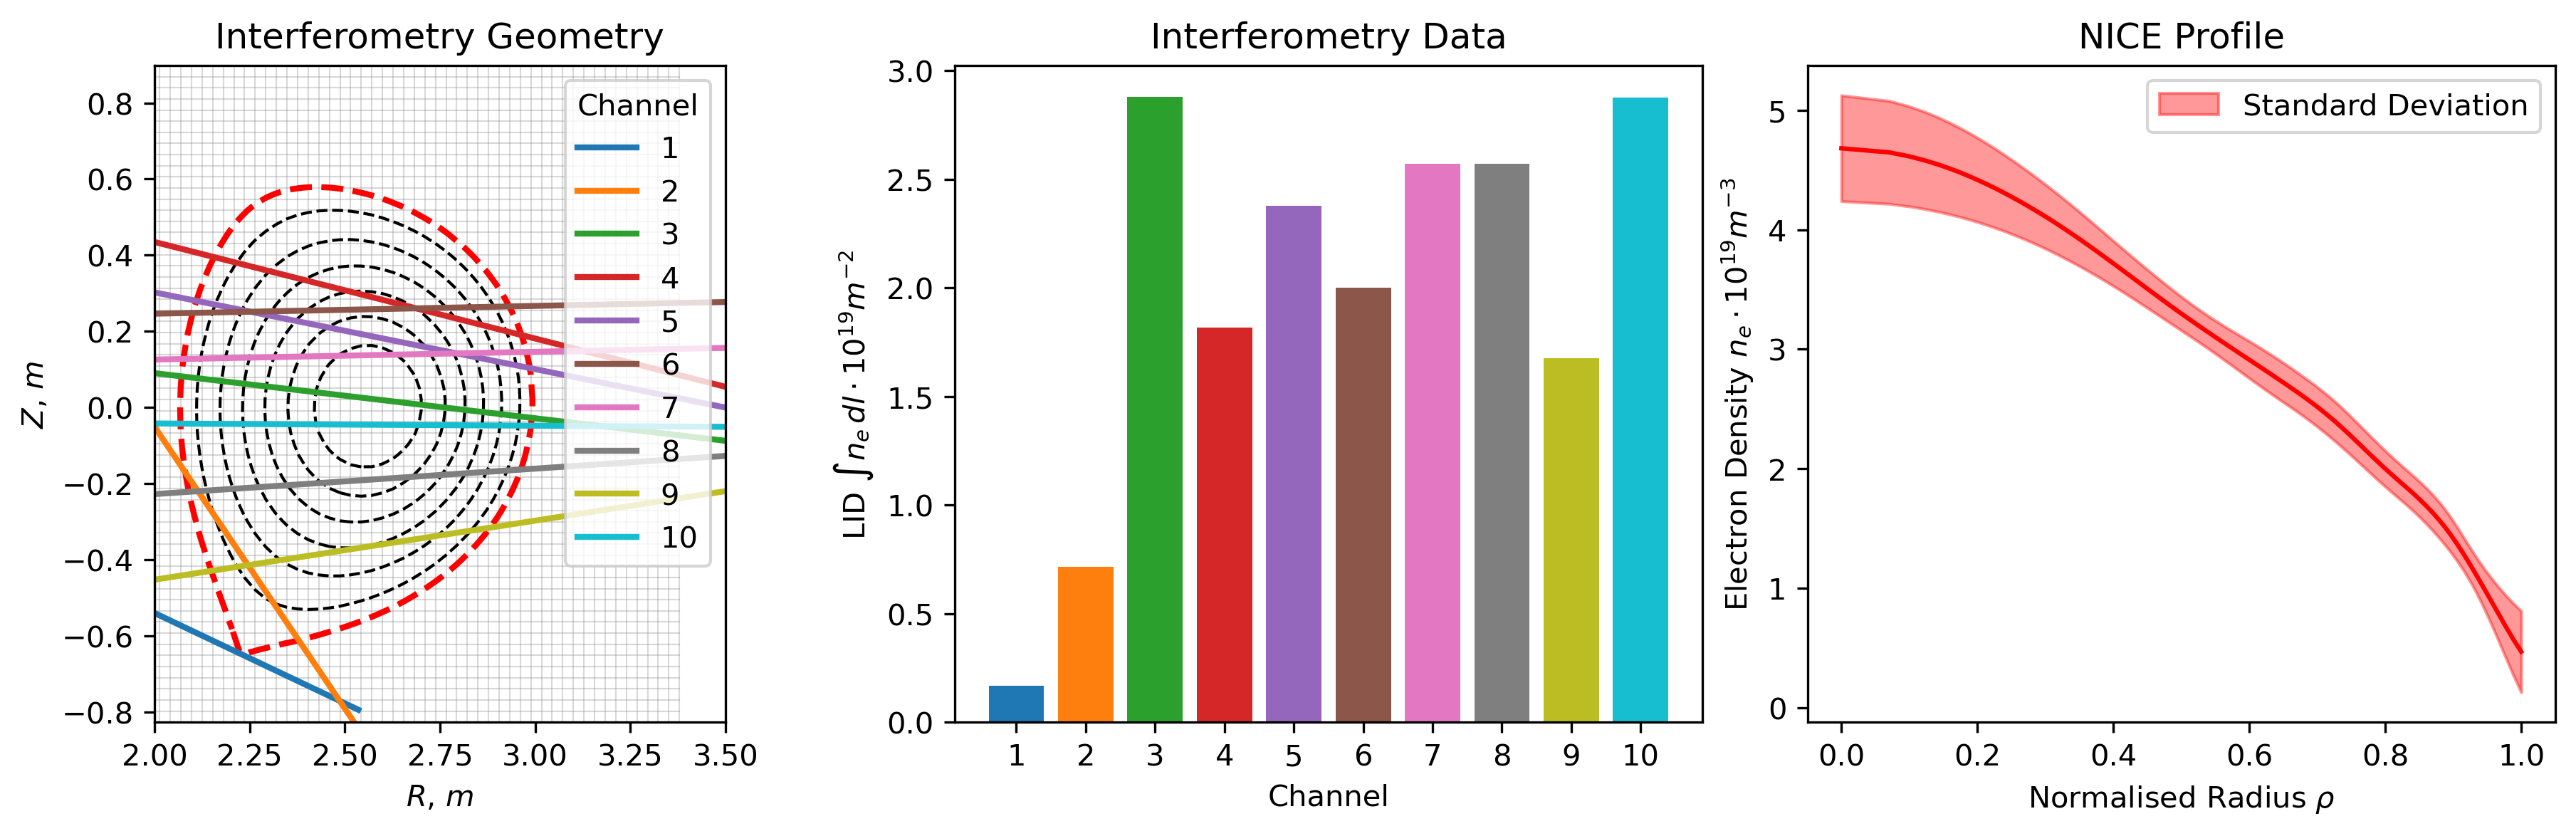
\includegraphics[width=500pt]{images/Final/interferometry_nice.png}
    \caption{A typical set of magnetic flux surfaces and interferometry data from the WEST tokamak. The electron desnity profile inferred by the NICE algorithem.}
    \label{fig:interf_nice}
\end{figure}

\begin{figure}[ht]
    \centering
    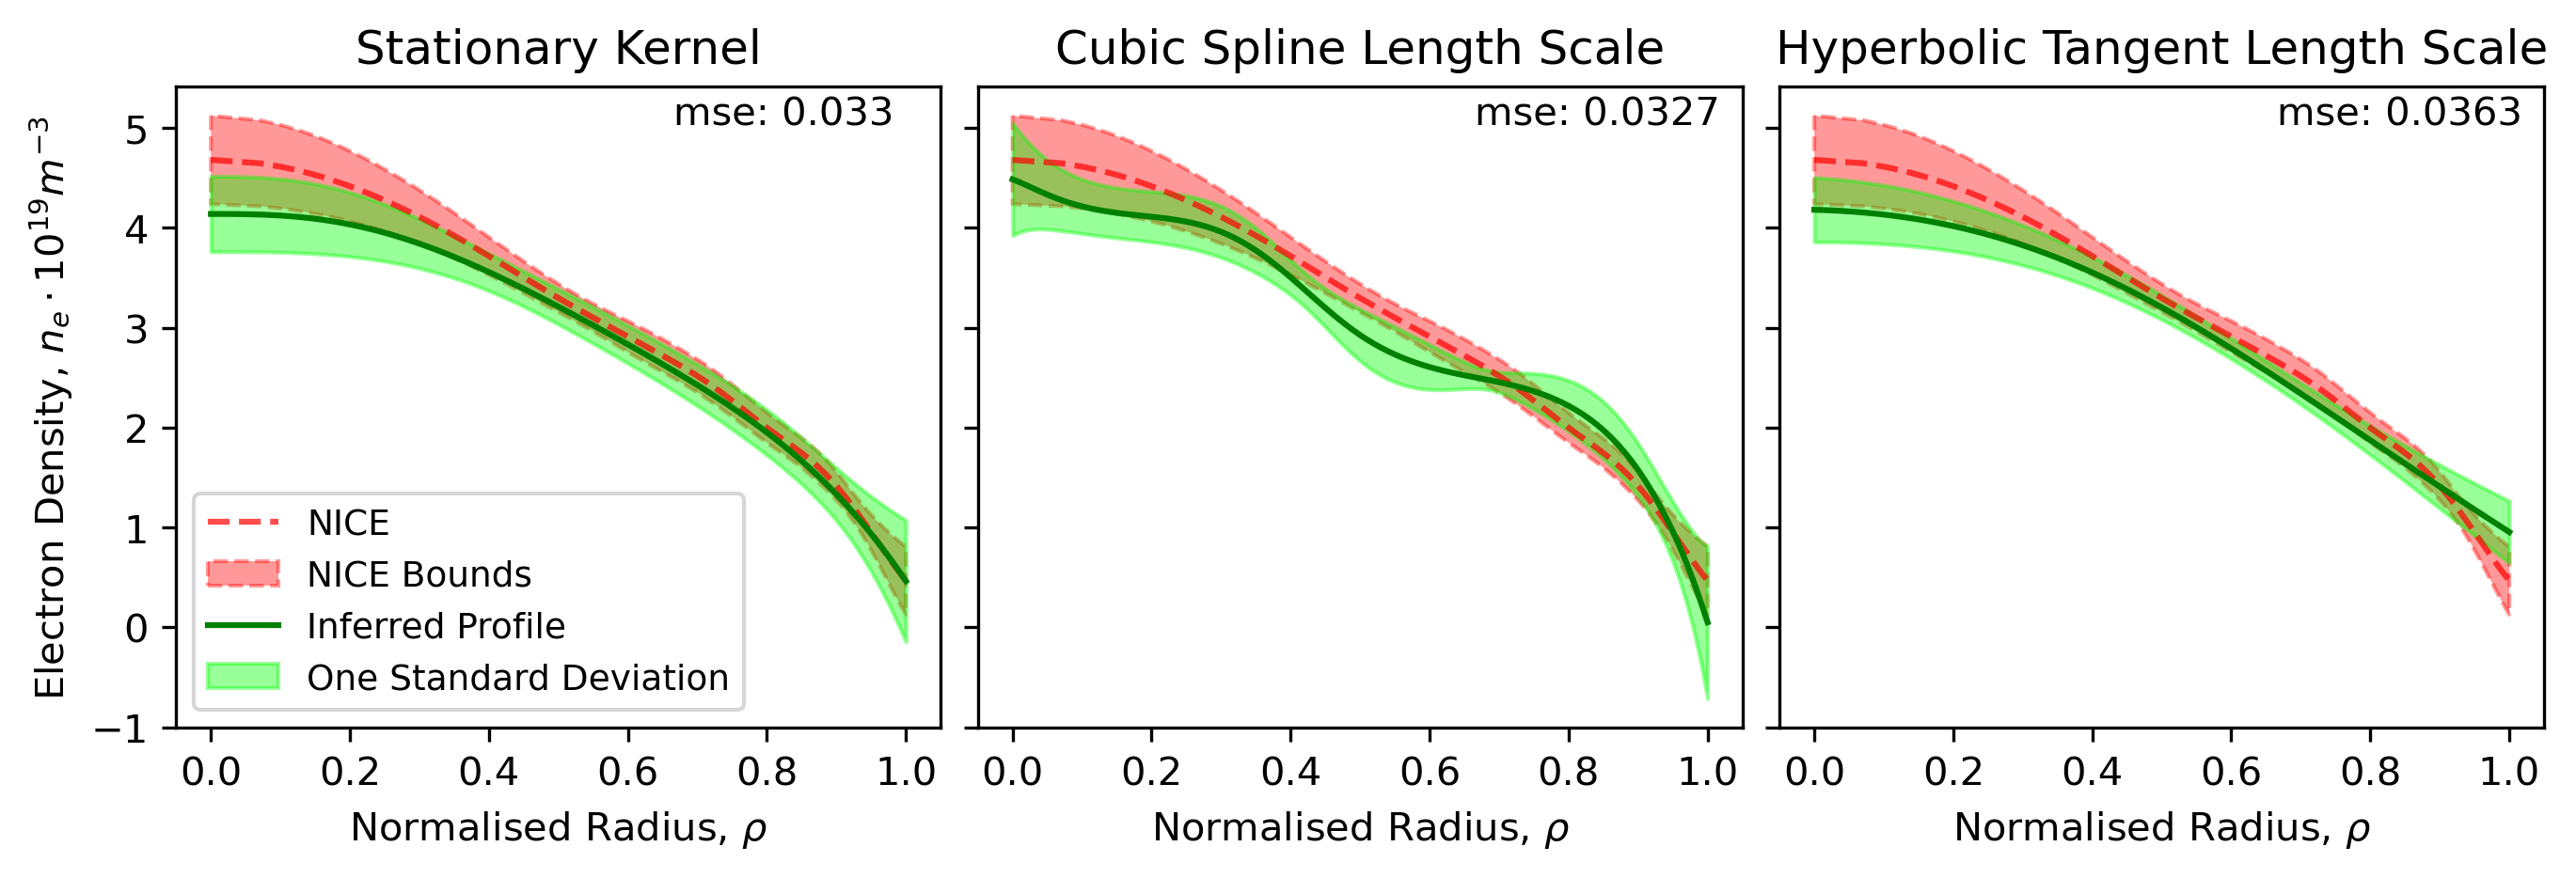
\includegraphics[width=\textwidth]{images/Final/NICE_real_map_likep.png}
    \caption{Electron density inference using the hyperparameter MAP method on real interferometry data from the WEST tokamak. The mean square error is shown as `mse'.}
    \label{fig:map_real}
\end{figure}

% \begin{figure}[ht]
%     \centering
%     \includegraphics[width=\textwidth]{images/Final/NICE_real_fb_likep.png}
%     \caption{Electron density inference using the full Bayesian method on real interferometry data from the WEST tokamak. The mean square error is shown as `mse'.}
%     \label{fig:map_real}
% \end{figure}




% \begin{table}
% \centering
% \begin{tabular}{|c|c|c|}
%     \hline
%     \textbf{Hyperparameter} & \textbf{Lower Bound} & \textbf{Upper Bound} \\
%     \hline
%     Amplitude & 0 & 100 \\
%     Length Scale & 0 & 3 \\
%     \hline
%     \textbf{Hyperbolic Tangent} & &\\
%     Transition Center & 0 & 1 \\
%     Transition Width & 0.01 & 0.5 \\
%     \hline
%     \textbf{Cubic Spline} & & \\
%     5 Knots Evenly Spaced in $rho$ & & \\
%     \hline
% \end{tabular}
% \caption{}
% \label{tbl:prior}
% \end{table}

%methodology

% Explain the details of the how the theory is implimented, what processing power is required, I used python jupyter notebooks numpy, scipy and pytorch. Explain the key parts of the code in order to compute the kernels, marginal likelyhood and inference. What test were done in order to try and improve the inference. 

% \begin{itemize}
%     \item What format was the data in when it came from west and how did I import it into python
%     \item A bit about the diffent forms the data comes in on the west imas database and which one was chosen. 
%     \item How can the accuracy of the forward model be tested and how should this effect the experimental error.
%     \item How does one select an experimental error, is it important for the inference? 
%     \item What is the non positive definite matrix error, how can it be avoided, what are the implications of this
%     \item How I used meshgrid to compute the kernel in a fast way
%     \item what are the different methods used for finding the minimum of the marginal likelyhood, scipy minimize, pytorch, grid search. How do they work. 
%     \item What distributions did I use to randomly initialize the kernel parameters. Why did I randomly initialise them?
%     \item Why I coded everything with pytorch tensors
%     \item How I optimised the learning rate
%     \item Attempts to use noise
%     \item How did I try and improve the inference.
%     \item summarise the chapter and lead into the results. 
    
% \end{itemize}


% \begin{itemize}
%     \item Make the case as why a 0 mean prior is not always a good Idea, since the marginal likelyhood is not perfect and inferences favour the lower side of NICE, likely due to the 0 prior as when amp is increased the inference will move to NICE but not beyond it. Including prior knowledge when available is always advised.
    
%     \item Make the case that if I set NICE as the true ground truth and create synthetic data then I get the NICE profile from lowering marginal likelyhood. This shows that everything is set up correctly.
    
%     \item Show I am getting a local minimum of the marginal likelihood which is nice like and a lower minimum which is parabolic. This could be a result of the marginal likelihood not being a perfect loss function for problems with little data. This seems to be true for SciPy, PyTorch, static and non-static.
%     \item Talk about the discovered more defined ridge, ask for access to log book to see if this is during a H-mode shot. Explain why it might be physically significant but a full monte carlo bayesian should be carried out to verify this. 
%     \item Show the static grid search

%     \item Results not yet curated
%         \subitem Bayesian inference using monte carlo methods
%         \subitem One size fits all kernel for real time. 
%     \item summarise the chapter and lead into conclusions
% \end{itemize}




%Figure \ref{fig:trace6000} shows a trace plot for the static lengthscale samples from a 6000 sample chain. 
% \begin{figure}[ht]
%     \centering
%     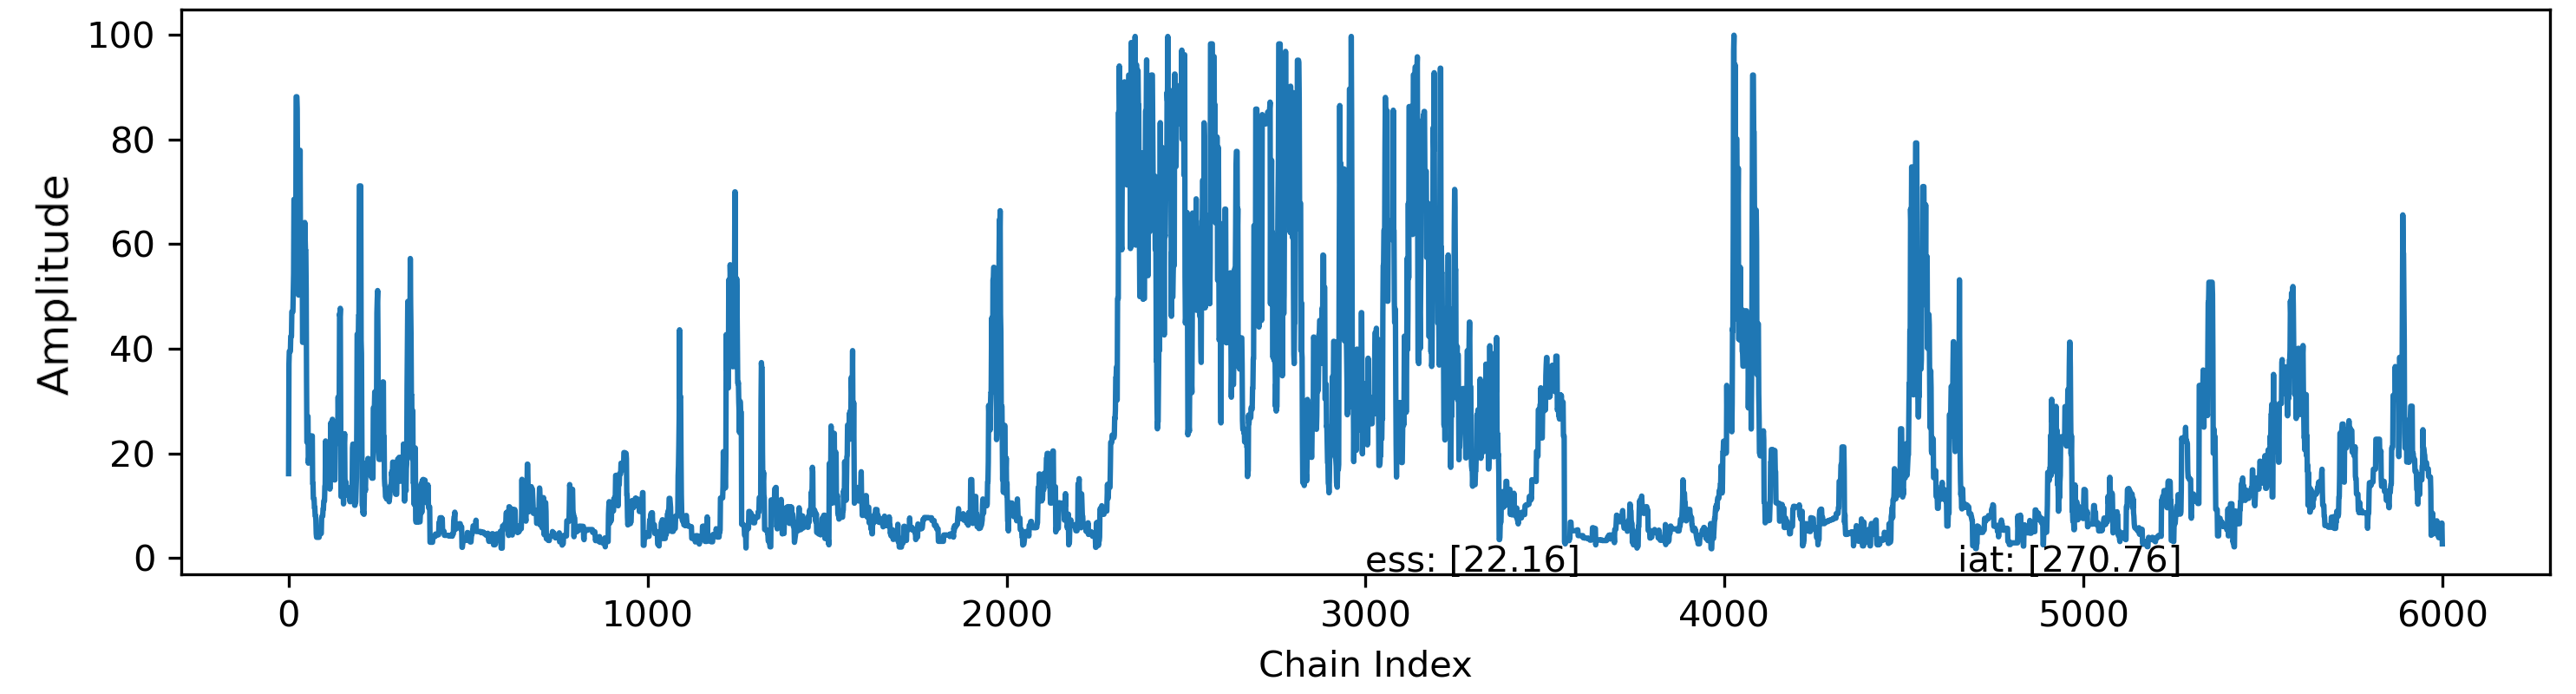
\includegraphics[width=\textwidth]{images/Final/Trace.png}
%     \caption{A trace plot showing the 6000 amplitude samples taken by an emcee chain. The integrated autocorrelation time and effective sample size is shown as `iat' and `ess', respectivly.}
%     \label{fig:trace6000}
% \end{figure}
\chapter{Conclusion}

The tokamak is the most researched device that has the highest chance of becoming a viable fusion reactor.  Within the tokamak, it is vital to be able to measure the electron density throughout the device to ensure safety limits are maintained and fusion performance goals are met. The equilibrium of the tokamak plasma has toroidally symmetric flux surfaces on which the electron density is constant. The flux surfaces allow a 1D electron density profile to express the density throughout the tokamak. The flux surfaces are provided by the \gls{nice} code which uses magnetic diagnostic data to determine the flux surfaces. There are multiple diagnostics that can measure the electron density. This thesis focused on the interferometry diagnostic within the \gls{west} tokamak. Interferometry is a technique that uses the optical path length difference of vacuum to plasma for multiple lasers fired through the plasma to determine the line integrated electron density along the laser's line of sight. This can provide enough information to infer the electron density profile with Bayesian techniques. Both real and synthetic data were used to test various Bayesian techniques. The various techniques were different ways to deal with the hyperparameters that defined the prior. Three different kernels were trialled that defined the functional form of the smoothness of the final inferred profile. The parameters in the kernels were decided using a \gls{map} of the hyperparameter posterior or with a full Bayesian analysis which involves marginalising the hyperparameters by sampling from a joint probability distribution of the electron density profiles posterior and the hyperparameter posterior. Once the hyperparameters are known then the posterior of the density profile can be computed analytically; although this process requires matrix inversion. The prior information also included that we know the gradient is close to 0 in the core and the density is close to 0 at the last closed flux surface. This was included in the Bayesian analysis using artificial observations. \gls{nice} also provides an electron density profile for real \gls{west} shots and can be compared to the Bayesian methods.

Five synthetic profiles were defined and used to create synthetic interferometry data. These included L-mode, H-mode, Peaked, L-mode Peaked and H-mode Peaked. They are all scientifically relevant profile shapes. Real interferometry data from a typical \gls{west} shot was also used. The inferred profiles of the synthetic data could be compared to the synthetic profiles and the inferred profiles from the real data could be compared to the \gls{nice} profile. The full Bayesian approach involves \gls{mcmc} sampling which was carried out using the emcee python package. The emcee parameters are turned to minimise the autocorrelation. There was still substantial autocorrelation that reduced the reliability of the samples to be from the true hyperparameter posterior distribution. This reduces the credibility of this implementation of the full Bayesian approach. The final inferences show potential for the methods explored but are inconclusive as to which is the best method. There was no combination of the kernels and hyperparameter method that was able to perform well on all of the profiles of interest. A few of the inferences very well match the synthetic or \gls{nice} profile; although for a real scenario, there is no comparison profile to assess performance and the inference algorithm must be able to cope with any ground truth profile.

For future investigation, more optimisation techniques could be deployed for finding the \gls{map} of the hyperparameter posterior of the various kernels. The cubic spline function for the hyperbolic tangent was the most flexible function used which should allow it to be the most effective for a wide variety of profiles, the number of spline knots and their prior positions could be better tuned to improve performance. The amplitude hyperparameter determines how far from the prior profile the inference can easily go. This is an intuitive parameter that could potentially be manually selected to reduce the dimensionality of the parameter space to be searched and increase the chance an optimal length-scale function could be selected. \gls{west} also collects polarimetry data and this also contains information about the electron density profile. More work could be done to include this information in the Bayesian inference. This would involve using the temperature profile to get the current profile which could be used to get the poloidal magnetic field which could then separate the electron density from the poloidal magnetic field in the polarimetry phase shift shown in equation, \ref{eq:pol_farad}. There is also information available about the amount of fuel injected into the system and this is correlated to the electron density. This could be used to get a more accurate prior for the electron density profile. Once the algorithm is stable and consistently provides accurate inferences then the next step would be to test the real-time capabilities. The slowest process is the hyperparameter optimisation and after that the matrix inversion. Perhaps these could be replaced with reduced models or neural networks to ensure real-time computation speeds.


\chapter{Future Investigation}

% \begin{itemize}
%     \item In future the injected gas information could be included to get a prior mean vector. How does this affect the inference? Is the widely accepted 0 mean prior a good idea? Simply make the prior mean high enough so that 99\% of the area is in the positive region. Since we know that the electron density is certainly positive. 
%     \item Plolarimetry information could be included. Using a thermal profile to get current profile to get polodial magnetic field profile to then use the polarimetry measurements to get more data on the current density. Explain why NICE didn't do this and why this might allow another implementation to improve on NICE.
%     \item try maximizing likelyhood rather than marginal likelyhood for best parameters. See obsidian closely fitting the data. 
%     \item Full monte carlo if not done, to get a bayesian ground truth.
%     \item Explain potential for real time inference, why its is important and how you envision it could be done. Using data from many shots and times we could compute the least square error of inference with bayesian ground truth as the loss function to optimise a one size fits all kernel with many parameters. Each l(rho) and sigma(rho) has a different value then the kernel would only have sigma along the diagonal as l can be optimized on the off diagonals to account for different sigma values. This reduces the chance of non positive definite matrix errors. Then using posterior of one inference as prior of next. Why is this method better than a neural network?
%     \item Jeffry finds the parameters are the same for many shots, he thinks I can take the mean and it will work fine as a one size fits all kernel.
%     \item Jeffries Advanced Static Kernel, a reference prior can be used to direct the functional form limitations of a non static kernel which is the Advanced Static Kernel.  The reference prior could be NICE, A monte carlo inference for 1 shot, or a parabolic with correct core and edge with edge being 0 and core given by amount of gas injected. It just needs to follow the rough shape as the implimentation is general. Although I fear if I use a parabolic the inferences will be parabolic. 
%     \item Jeffries Advanced Static Kernel could be used to help get a one size fits all kernel. You could learn the $sigma_{ij}$ and $l_{ij}$ that lead to the lowest loss over many shots and you don't need to worry about non positive definite errors as $sigma_{ij}$ and $l_{ij}$ are fed into the the Advanced static kernel formula. Then you have very many parameters as 
%  \end{itemize}

%----------------------------------------------------------------------
% END MATERIAL
% Bibliography, Appendices, Index, etc.
%----------------------------------------------------------------------

% Bibliography

% The following statement selects the style to use for references.  
% It controls the sort order of the entries in the bibliography and also the formatting for the in-text labels.
\bibliographystyle{plain}
% This specifies the location of the file containing the bibliographic information.  
% It assumes you're using BibTeX to manage your references (if not, why not?).
\cleardoublepage % This is needed if the "book" document class is used, to place the anchor in the correct page, because the bibliography will start on its own page.
% Use \clearpage instead if the document class uses the "oneside" argument
\phantomsection  % With hyperref package, enables hyperlinking from the table of contents to bibliography             
% The following statement causes the title "References" to be used for the bibliography section:
\renewcommand*{\bibname}{References}

% Add the References to the Table of Contents
\addcontentsline{toc}{chapter}{\textbf{References}}

\bibliography{uw-ethesis.bib}
% Tip: You can create multiple .bib files to organize your references. 
% Just list them all in the \bibliogaphy command, separated by commas (no spaces).

% The following statement causes the specified references to be added to the bibliography even if they were not cited in the text. 
% The asterisk is a wildcard that causes all entries in the bibliographic database to be included (optional).
\nocite{*}
%----------------------------------------------------------------------

% Appendices

% The \appendix statement indicates the beginning of the appendices.
\appendix
% Add an un-numbered title page before the appendices and a line in the Table of Contents
\chapter*{APPENDICES}/
\addcontentsline{toc}{chapter}{APPENDICES}
% Appendices are just more chapters, with different labeling (letters instead of numbers).
\chapter{Deriving the Closed Form Posterior Expressions}
% \label{Appendix A}
\label{append:dervcf}
The inference begins with Bayes theorem,  

\begin{equation}    
    P(\vec{y}|\vec{d}, \vec\epsilon, \theta) = \frac{P(\vec{d}|\vec{y},\vec\epsilon)P(\vec{y}|\theta)}{P(\vec d|\vec\epsilon,\theta)},
\end{equation}

\noindent where the likelihood can be written as,

\begin{equation}
P(\vec{d}|\vec{y},\vec\epsilon) = \frac{1}{(2\pi)^{\frac{m}{2}} \sqrt{|\Sigma_{li}|}} \exp \left[ -\frac{1}{2} (\vec d - R\vec y)^{\top} \Sigma^{-1}_{li} (\vec d - R\vec y) \right], \, \Sigma_{li} = \vec \epsilon I,
\end{equation}

\noindent the prior as,

\begin{equation}
\begin{split}
P(\vec y|\theta) = \frac{1}{(2\pi)^{\frac{n}{2}} \sqrt{|K|}} \exp \left[ -\frac{1}{2}(\vec y - \vec \mu_{pr})^{\top} K^{-1} (\vec y - \vec \mu_{pr}) \right],\\
\theta \rightarrow \{\sigma, l\}, \, K_{ij} = k(\rho_i, \rho_j) = \sigma^2 \exp \left[\frac{(\rho_i - \rho_j)^2}{2l^2}\right],
\end{split}
\end{equation}

\noindent and the posterior as,

\begin{equation}
P(\vec{y}|\vec{d},\vec\epsilon, \theta) = \frac{1}{(2\pi)^{\frac{n}{2}} \sqrt{|\Sigma_{post}|}} \exp \left[ -\frac{1}{2}(\vec y - \mu_{post})^{\top} \Sigma^{-1}_{post} (\vec y - \vec{\mu}_{post}) \right].
\end{equation}

\noindent To derive $\vec{\mu}_{post}$ and $\Sigma_{post}$ the likelihood and prior are multiplied together and re-arranged. Only first and second order $\vec y$ terms are kept as the constants do not affect the shape of the multivariate Gaussian and thus do not affect $\vec{\mu}_{post}$ or $\Sigma_{post}$. Then using the completing the square formula for matrices they can be combined into a single multivariate Gaussian. By comparing with the posterior we find the closed form expressions for $\vec{\mu}_{post}$ and $\Sigma_{post}$. When the distributions are multiplied together the exponential powers are summed,

$$
 -\frac{1}{2}\left[(\vec d - R\vec y)^{\top} \Sigma^{-1}_{li} (\vec d - R\vec y)  + (\vec y - \vec \mu_{pr})^{\top} K^{-1} (\vec y - \vec \mu_{pr})\right],
$$

\noindent ignoring the $-\frac{1}{2}$ for now and multiplying it out gets,

\begin{multline*}
\left(\vec d ^\top \Sigma_{li}^{-1} \vec d - \vec d^\top \Sigma_{li}^{-1} R\vec y - (R\vec y)^\top \Sigma_{li}^{-1} \vec d + (R\vec y)^\top \Sigma_{li}^{-1} R\vec y \right), \\ 
+ \left( \vec y^\top K^{-1} \vec y - \vec y^\top K^{-1} \vec \mu_{pr} - \vec \mu_{pr}^\top K^{-1} \vec y + \vec \mu_{pr}^\top K^{-1} \vec \mu_{pr} \right),
\end{multline*}

\noindent focusing on the $1^{st}$ order terms and remembering that the transpose of a scalar is itself and the transpose of a symmetric matrix (e.g. $\Sigma_{li}$) is itself, it can be shown that the first order terms equate to

$$
- \vec d^\top \Sigma_{li}^{-1} R\vec y - (R\vec y)^\top \Sigma_{li}^{-1} \vec d - \vec y^\top K^{-1} \vec \mu_{pr} - \vec \mu_{pr}^\top K^{-1} \vec y = -2 \vec y^\top ( R^{\top} \Sigma_{li}^{-1}\vec d + K^{-1} \vec \mu_{pr}) =-2 \vec y^\top \vec b
$$

\noindent in which a substitution was made to ease the use of the competing square formula, 

$$
\vec b = R^{\top} \Sigma_{li}^{-1}\vec d + K^{-1} \vec \mu_{pr}
$$

\noindent switching the focus to the $2^{nd}$ order terms,

$$
(R\vec y)^\top \Sigma_{li}^{-1} R\vec y + \vec y^\top K^{-1} \vec y = \vec y^\top (R^\top \Sigma_{li}^{-1} R + K^{-1}) \vec y = \vec y^\top M \vec y,
$$

\noindent in which a substitution was made to ease the use of the completing square formula,

$$
M = (R^\top \Sigma_{li}^{-1} R + K^{-1})
$$

\noindent ignoring 0 order terms that do not affect the shape, the original exponential power takes the form,

$$
 -\frac{1}{2}\left[\vec y^\top M \vec y - \vec y^\top \vec b \right],
$$

\noindent by completing the squares we obtain
$$
\vec y^\top M \vec y - y^\top \vec b = (\vec y - M^{-1}\vec b)^\top M (\vec y - M^{-1} \vec b) - \vec b^\top M^{-1} \vec b.
$$

\noindent We can ignore $\vec b^\top M^{-1} \vec b$ as it doesn't affect the shape of the Gaussian. Finally, for the posterior we have

$$
P(\vec{y}|\vec{d},\vec\epsilon, \theta) \propto \exp \left[ -\frac{1}{2}(\vec y - \vec{\mu}_{post})^{\top} \Sigma^{-1}_{post} (\vec y - \vec{\mu}_{post}) \right] \propto \exp \left[ -\frac{1}{2} (\vec y - M^{-1}\vec b)^\top M (\vec y - M^{-1} \vec b)\right],
$$

\noindent from comparison, it can be seen that,

\begin{equation}
\vec{\mu}_{post} = M^{-1} \vec b = \left(R^\top \Sigma_{li}^{-1} R + K^{-1}\right)^{-1} \left(R^{\top} \Sigma_{li}^{-1}\vec d + K^{-1} \vec \mu_{pr}\right), \, \Sigma_{post} = M^{-1} = \left(R^\top \Sigma_{li}^{-1} R + K^{-1}\right)^{-1}.
\end{equation}

\noindent The posterior mean is often written in another form. This form can be found with the following steps,

$$
\begin{aligned}
\vec{\mu}_{post} &= (K^{-1} + R^{\top} \Sigma_{li}^{-1} R)^{-1}(R^{\top} \Sigma_{li}^{-1} \vec{d} + K^{-1} \vec{\mu}_{pr}) \\
&= (K^{-1} + R^{\top} \Sigma_{li}^{-1} R)^{-1} R^{\top} \Sigma_{li}^{-1} \vec{d} + (K^{-1} + R^{\top} \Sigma_{li}^{-1} R)^{-1} (K^{-1} + R^{\top} \Sigma_{li}^{-1} R - R^{\top} \Sigma_{li}^{-1} R) \vec{\mu}_{pr} \\
&= \vec{\mu}_{pr} + (K^{-1} + R^{\top} \Sigma_{li}^{-1} R)^{-1} R^{\top} \Sigma_{li}^{-1} \vec{d} - (K^{-1} + R^{\top} \Sigma_{li}^{-1} R)^{-1} R^{\top} \Sigma_{li}^{-1} R \vec{\mu}_{pr} \\
&= \vec{\mu}_{pr} + (K^{-1} + R^{\top} \Sigma_{li}^{-1} R)^{-1} R^{\top} \Sigma_{li}^{-1} (\vec{d} - R \vec{\mu}_{pr}).
\end{aligned}
$$

\noindent The final closed form expression of the posterior mean and covariance is

\begin{gather}
\vec{\mu}_{post}= \vec{\mu}_{pr} + (K^{-1} + R^{\top} \Sigma_{li}^{-1} R)^{-1} R^{\top} \Sigma_{li}^{-1} (\vec{d} - R \vec{\mu}_{pr})\\
\Sigma_{post} = \left(R^\top \Sigma_{li}^{-1} R + K^{-1}\right)^{-1}.
\end{gather}

\noindent The error of each value in $\vec{\mu}_{post}$ can be found on the diagonal of $\Sigma_{post}$.

\chapter{Deriving the Marginal Likelihood and Loss Function Expression}
% \label{Appendix B}
\label{append:dervml}

The marginal likelihood is the denominator in Bayes theorem for the inference

\begin{equation}
P(\vec{y}|\vec{d}, \vec\epsilon, \theta) = \frac{P(\vec{d}|\vec{y},\vec\epsilon)P(\vec{y}|\theta)}{P(\vec d|\vec\epsilon,\theta)},
\end{equation}

\noindent since the marginal likelihood is a normalizing constant it can be expressed as

\begin{equation}
P(\vec d|\vec\epsilon,\theta) = \int P(\vec{d}|\vec{y},\vec\epsilon)P(\vec{y}|\theta)  \, d\vec y,
\end{equation}

\noindent the likelihood is,

\begin{equation}
P(\vec{d}|\vec{y},\vec\epsilon) = \frac{1}{(2\pi)^{\frac{m}{2}} \sqrt{|\Sigma_{li}|}} \exp \left[ -\frac{1}{2} (\vec d - R\vec y)^{\top} \Sigma^{-1}_{li} (\vec d - R\vec y) \right], \hspace{0.5cm} \Sigma_{li} = \vec \epsilon I,
\end{equation}

\noindent and the prior is,

\begin{equation}
\begin{split}
P(\vec y|\theta) = \frac{1}{(2\pi)^{\frac{n}{2}} \sqrt{|K|}} \exp \left[ -\frac{1}{2} (\vec y - \vec \mu_{pr})^{\top} K^{-1} (\vec y - \vec \mu_{pr}) \right],\\
\theta \rightarrow \{\sigma, l\}, \hspace{0.5cm} K_{ij} = k(\rho_i, \rho_j) = \sigma \exp \left[\frac{\rho_i - \rho_j}{2l^2}\right],
\end{split}
\end{equation}

\noindent when multiplied together the exponential powers become 

\begin{multline*}
\left(\vec d ^\top \Sigma_{li}^{-1} \vec d - \vec d^\top \Sigma_{li}^{-1} R\vec y - (R\vec y)^\top \Sigma_{li}^{-1} \vec d + (R\vec y)^\top \Sigma_{li}^{-1} R\vec y \right)\\ 
+ \left( \vec y^\top K^{-1} \vec y - \vec y^\top K^{-1} \vec \mu_{pr} - \vec \mu_{pr}^\top K^{-1} \vec y + \vec \mu_{pr}^\top K^{-1} \vec \mu_{pr} \right),
\end{multline*}

\noindent the first order terms of $\vec y$ can be simplified,

$$
-\vec d^\top \Sigma_{li}^{-1} R\vec y - (R\vec y)^\top \Sigma_{li}^{-1} \vec d - \vec y^\top K^{-1} \vec \mu_{pr} - \vec \mu_{pr}^\top K^{-1} \vec y = -2 \vec y^\top ( R^{\top} \Sigma_{li}^{-1}\vec d + K^{-1} \vec \mu_{pr}) =-2 \vec y^\top \vec b,
$$

\noindent the second order terms of $\vec y$ can be simplified,

$$
(R\vec y)^\top \Sigma_{li}^{-1} R\vec y + \vec y^\top K^{-1} \vec y = \vec y^\top (R^\top \Sigma_{li}^{-1} R + K^{-1}) \vec y = \vec y^\top M \vec y,
$$

\noindent all together, for the marginal likelihood we have

\begin{equation}
\begin{aligned}
 P(\vec d|\vec\epsilon,\theta) 
 &= \int P(\vec{d}|\vec{y},\vec\epsilon)P(\vec{y}|\theta)  \, d\vec y \\
 &= \frac{1}{(2\pi)^{\frac{m}{2}} \sqrt{|\Sigma_{li}|}} \frac{1}{(2\pi)^{\frac{n}{2}} \sqrt{|K|}} \exp\left[ -\frac{1}{2}(\vec d ^\top \Sigma_{li}^{-1} \vec d + \vec \mu_{pr}^\top K^{-1} \vec \mu_{pr} )\right] \int \exp\left[-\frac{1}{2}\vec y^\top M \vec y + \vec y^\top \vec b\right] \, d\vec y, 
\end{aligned}
\end{equation}

\noindent performing a standard Gaussian integral we get that

$$
\int \exp\left[-\frac{1}{2}\vec y^\top M \vec y + \vec y^\top \vec b\right] \, d\vec y =  \frac{(2\pi)^\frac{n}{2}}{\sqrt{|M|}} \exp \left[ \frac{1}{2} \vec b^\top M^{-1}\vec b \right],
$$

\noindent all together, for the marginal likelihood we have

$$
\begin{aligned}
 P(\vec d|\vec\epsilon,\theta) &= \int P(\vec{d}|\vec{y},\vec\epsilon)P(\vec{y}|\theta)  \, d\vec y\\
 &= \frac{(2\pi)^{\frac{n}{2}}}{(2\pi)^{\frac{m}{2}} (2\pi)^{\frac{n}{2}} \sqrt{|\Sigma_{li}||K||M|}} \exp\left[ -\frac{1}{2}(\vec d ^\top \Sigma_{li}^{-1} \vec d + \vec \mu_{pr}^\top K^{-1} \vec \mu_{pr} - \vec b^\top M^{-1}\vec b )\right],
\end{aligned}
$$

\noindent where $\vec b$ and $M$ are substitutions made earlier
$$
\vec b = R^{\top} \Sigma_{li}^{-1}\vec d + K^{-1} \vec \mu_{pr}
$$
$$
M = (R^\top \Sigma_{li}^{-1} R + K^{-1}),
$$

\noindent ignoring the $-\frac{1}{2}$ for now and reverting $\vec b$ and $M$ to their original form the exponential power becomes

$$
\vec{\mu}_{pr}^{\top} K^{-1} \vec{\mu}_{pr} + \vec{d}^{\top} \Sigma_{li}^{-1} \vec{d}- (R^{\top} \Sigma_{li}^{-1} \vec{d} + K^{-1}\vec{\mu}_{pr})^{\top} (K^{-1} + R^{\top} \Sigma_{li}^{-1} R)^{-1} (R^{\top} \Sigma_{li}^{-1} \vec{d} + K^{-1}\vec{\mu}_{pr}),
$$

\noindent the next step requires the Woodbury identity \cite{gp4ml}, 

\begin{equation}
(A + UCV)^{-1} = A^{-1} - A^{-1}U(C^{-1}+VA^{-1}U)^{-1}VA^{-1},
\end{equation}

\noindent the exponential power can thus be expanded to be
$$
\vec{\mu}_{pr}^{\top} K^{-1} \vec{\mu}_{pr} + \vec{d}^{\top} \Sigma_{li}^{-1} \vec{d} - (R^{\top} \Sigma_{li}^{-1} \vec{d} + K^{-1}\vec{\mu}_{pr})^{\top} \left[K - K R^{\top} \left(\Sigma_{li} + RK R^{\top}\right)^{-1} R K \right] (R^{\top} \Sigma_{li}^{-1} \vec{d} + K^{-1}\vec{\mu}_{pr}),
$$

\noindent This can then be rearranged to be

\begin{multline*}
\vec{d}^{\top} \left\{ \Sigma_{li}^{-1} - \Sigma_{li}^{-1} R \left[K - K R^{\top} \left(\Sigma_{li} + RK R^{\top}\right)^{-1} R K \right] R^{\top} \Sigma_{li}^{-1} \right\} \vec{d} \\- 2 \vec{\mu}^{\top} K^{-1} \left[K - K R^{\top} \left(\Sigma_{li} + RK R^{\top}\right)^{-1} R K \right] R^{\top} \Sigma_{li}^{-1} \vec{d} \\+ \vec{\mu}^{\top} \left\{ K^{-1} - K^{-1}\left[K - K R^{\top} \left(\Sigma_{li} + RK R^{\top}\right)^{-1} R K \right] K^{-1} \right\}\vec{\mu},
\end{multline*}

\noindent the second order term in $\vec d$ can be reduced

$$
\begin{aligned}
\Sigma_{li}^{-1} - \Sigma_{li}^{-1} R &\left[K - K R^{\top} \left(\Sigma_{li} + RK R^{\top}\right)^{-1} R K \right] R^{\top} \Sigma_{li}^{-1} \\ &= \Sigma_{li}^{-1} - \Sigma_{li}^{-1} R K R^{\top} \Sigma_{li}^{-1} + \Sigma_{li}^{-1} R K R^{\top} \left(\Sigma_{li} + RK R^{\top}\right)^{-1} R K R^{\top} \Sigma_{li}^{-1}\\ &= \Sigma_{li}^{-1} - \Sigma_{li}^{-1} R K R^{\top} \Sigma_{li}^{-1} + \Sigma_{li}^{-1} \left(\Sigma_{li} + R K R^{\top} - \Sigma_{li}\right)\left(\Sigma_{li} + RK R^{\top}\right)^{-1} R K R^{\top} \Sigma_{li}^{-1} \\
&= \Sigma_{li}^{-1} - \left(\Sigma_{li} + RK R^{\top}\right)^{-1} R K R^{\top} \Sigma_{li}^{-1} \\ &= \Sigma_{li}^{-1} - \left(\Sigma_{li} + RK R^{\top}\right)^{-1} \left(\Sigma_{li} + R K R^{\top} - \Sigma_{li} \right)\Sigma_{li}^{-1} \\ &= \left(\Sigma_{li} + RK R^{\top}\right)^{-1},
\end{aligned}
$$

\noindent the first order term in $\vec d$ can be reduced
$$
\begin{aligned}
-2 \vec{\mu}^{\top} K^{-1} &\left[K - K R^{\top} \left(\Sigma_{li} + RK R^{\top}\right)^{-1} R K \right] R^{\top} \Sigma_{li}^{-1} \\
&= -2 \vec{\mu}^{\top} R^{\top} \Sigma_{li}^{-1} + 2 \vec{\mu}^{\top} R^{\top} \left(\Sigma_{li} + RK R^{\top}\right)^{-1} R K R^{\top} \Sigma_{li}^{-1}\\
&= -2 \vec{\mu}^{\top} R^{\top} \Sigma_{li}^{-1} + 2 \vec{\mu}^{\top} R^{\top} \left(\Sigma_{li} + RK R^{\top}\right)^{-1} \left( \Sigma_{li} + R K R^{\top} - \Sigma_{li} \right) \Sigma_{li}^{-1} \\
&= -2 \vec{\mu}^{\top} R^{\top} \Sigma_{li}^{-1} + 2 \vec{\mu}^{\top} R^{\top} \Sigma_{li}^{-1} - 2 \vec{\mu}^{\top} R^{\top} \left(\Sigma_{li} + RK R^{\top}\right)^{-1} \\
&= -2 \vec{\mu}^{\top} R^{\top} \left(\Sigma_{li} + RK R^{\top}\right)^{-1},
\end{aligned}
$$

\noindent the zero order term in $\vec d$ can be reduced 

$$
K^{-1} - K^{-1}\left[K - K R^{\top} \left(\Sigma_{li} + RK R^{\top}\right)^{-1} R K \right] K^{-1} = R^{\top} \left(\Sigma_{li} + RK R^{\top}\right)^{-1} R,
$$

\noindent now the exponential is 
$$
\begin{aligned}
\vec d ^\top \Sigma_{li}^{-1} \vec d + \vec \mu_{pr}^\top &K^{-1} \vec \mu_{pr} - \vec b^\top M^{-1}\vec b \\
&= \vec{d}^{\top} \left(\Sigma_{li} + RK R^{\top}\right)^{-1} \vec{d} -2 \vec{\mu}^{\top} R^{\top} \left(\Sigma_{li} + RK R^{\top}\right)^{-1} + \vec{\mu}^{\top} R^{\top} \left(\Sigma_{li} + RK R^{\top}\right)^{-1} R \vec{\mu} \\
&= (\vec{d} - R\vec{\mu}_{pr})^{\top} (\Sigma_{li} + R K R^{\top})^{-1} (\vec{d} - R\vec{\mu}_{pr}),
\end{aligned}
$$

\noindent the scaling constant can be simplified using the matrix determinant lemma \cite{gp4ml}, 

\begin{equation}
\lvert A + UCV \rvert = \lvert A \rvert \, \lvert C \rvert \, \lvert C^{-1} + V A^{-1} U \rvert,
\end{equation}

$$
|\Sigma_{li}||K||M| = |\Sigma_{li}||K||R^\top \Sigma_{li}^{-1} R + K^{-1}| = |\Sigma_{li} + RKR^\top|,
$$

this also helps avoid precision errors as there are fewer matrix inversions and determinants to compute. The marginal likelihood becomes

\begin{equation}
\begin{aligned}
 P(\vec d|\vec\epsilon,\theta) &= \int P(\vec{d}|\vec{y},\vec\epsilon)P(\vec{y}|\theta)  \, d\vec y \\
 &= \frac{1}{(2\pi)^{\frac{m}{2}} \sqrt{|\Sigma_{li} + RKR^\top|}} \exp\left[ -\frac{1}{2} (\vec{d} - R\vec{\mu}_{pr})^{\top} (\Sigma_{li} + R K R^{\top})^{-1} (\vec{d} - R\vec{\mu}_{pr}) \right].
\end{aligned}
\end{equation}

The values of the marginal likelihood can become very large and troublesome to compute with standard 64-bit float precision. For this reason, the logarithm is computed,

\begin{equation}
\ln(P(\vec d| \vec \epsilon,\theta)) = -\frac{1}{2} \left[m\ln(2\pi ) + \ln(|\Sigma_{li}+RKR^\top|) +  (\vec{d} - R\vec{\mu}_{pr})^{\top} (\Sigma_{li} + R K R^{\top})^{-1} (\vec{d} - R\vec{\mu}_{pr})\right]. 
\end{equation}

It is convention for loss functions to be minimized so the negative log marginal likelihood is used as the loss function for optimizing the hyper-parameters. When minimizing, the constants do not play a major role, thus the loss function for the hyperparameters is expressed as

\begin{equation}
loss(\epsilon, \theta) = \ln(|\Sigma_{li}+RKR^\top|) +  (\vec{d} - R\vec{\mu}_{pr})^{\top} (\Sigma_{li} + R K R^{\top})^{-1} (\vec{d} - R\vec{\mu}_{pr})
\end{equation}
\chapter{Complete Set of Distributions and Expressions for Reference}
\label{append:distexpres}
\section{Gaussian Process Regression for Interferometry, Discluding Artificial Observations}

In section \ref{sec:BIandSRP}, Bayesian inference was introduced for a simple regression problem. In section \ref{sec:InfForInterf} it was explained how to alter the method so that it could be applied to interferometry data to infer the electron density profile. Here are the mentioned distributions fully described for reference. The likelihood is,

\begin{equation}
\begin{aligned}
\mathcal{N}(\vec{d}, \vec{\mu_{li}} = R\vec{n_e}, \Sigma_{li}) &= \frac{1}{\sqrt{(2\pi)^{\frac{n}{2}}|\Sigma_{li}|}} \exp \left[{{-\frac{1}{2}(\vec{d}-R\vec{n_e})^\top\Sigma_{li}^{-1}(\vec{d}-R\vec{n_e})}}\right],\\
\Sigma_{li} = \vec{\epsilon}I &=
\begin{bmatrix}
\epsilon_1 & 0 & \cdots & 0\\
0 & \epsilon_2 & \cdots & 0\\
\vdots & \vdots & \ddots & 0 \\
0 & 0 & 0 &\epsilon_m
\end{bmatrix},
\end{aligned}
\end{equation}
  
\noindent where $R$ is a matrix composed of flux surface contribution row vectors, where each row vector corresponds to a different line of sight and when multiplied with $\vec{n_e}$ produces the line integrated density over that line of sight, see section \ref{sec:InfForInterf} for more details. The prior is,

\begin{equation}
\begin{aligned}
&\mathcal{N}(\vec{n_e}, \vec \mu_{pr} = \vec{0}, K) = \frac{1}{\sqrt{(2\pi)^{\frac{n}{2}}|K|}} \exp \left[{{-\frac{1}{2}\vec{n_e}^\top K^{-1}\vec{n_e}}}\right],\\
&K_{ij} = k(\rho_i, \rho_j) = \sigma^2 \left( \frac{2l(\rho_i)l(\rho_j)}{l(\rho_i)^2 + l(\rho_j)^2} \right)^{1/2} \exp\left({\frac{(\rho_i - \rho_j)^2}{l(\rho_i)^2+l(\rho_j)^2}}\right),\\
\end{aligned}
\end{equation}

\noindent where $l(\rho)$ can be a hyperbolic tangent function or otherwise. If $l$ is not a function but a constant, $l(\rho) = l$, then the kernel reverts back to the stationary kernel,

\begin{equation}
K_{ij} = k(\rho_i, \rho_j) = \sigma^2 \exp\left[{\frac{(\rho_i - \rho_j)^2}{2l^2}}\right],
\end{equation}
  
\noindent The goal is to compute the posterior,

\begin{equation}
\mathcal{N}(\vec{n_e}, \vec{\mu}_{post}, \Sigma_{post}) = \frac{1}{\sqrt{(2\pi)^{\frac{n}{2}}|\Sigma_{post}|}} \exp \left[{{-\frac{1}{2}(\vec{n_e}-\vec{\mu}_{post})^\top\Sigma_{post}^{-1}(\vec{n_e}-\vec{\mu}_{post})}}\right],\\
\end{equation}

\noindent which can be done with the closed form expressions,

\begin{gather}
    \vec{\mu}_{post}= \vec{\mu}_{pr} + (K^{-1} + R^{\top} \Sigma_{li}^{-1} R)^{-1} R^{\top} \Sigma_{li}^{-1} (\vec{d} - R \vec{\mu}_{pr})\\
    \Sigma_{post} = \left(R^\top \Sigma_{li}^{-1} R + K^{-1}\right)^{-1},
\end{gather}

\noindent as derived in appendix \ref{append:dervcf}. Once known the density profile can be plotted with the $\vec{\mu}_{post}$ values at the same $\rho$ values used in the kernel. The errors are the standard deviations held in the diagonal of $\Sigma_{post}$. This calculation is unlikely to be accurate until the hyperparameters are optimised. The parameters in the length scale function $l(\rho)$ are hyperparameters. The experimental errors $\epsilon$ can also be hyperparameters if unknown. The optimal hyperparameters can be found by minimising the negative log marginal likelihood. It is derived in appendix \ref{append:dervml} to be, 

\begin{equation}
loss(\vec \epsilon,\theta) = \ln(|\Sigma_{li}+RKR^\top|) + (\vec{d} - R\vec{\mu}_{pr})^{\top} (\Sigma_{li} + R K R^{\top})^{-1} (\vec{d} - R\vec{\mu}_{pr}).
\end{equation}

\noindent There is no change in its form from the simple regression problem. The values of the various matrices and vectors have changed. 

\section{Gaussian Process Regression for Interferometry, Including Artificial Observations}

Artificial observations can be placed in the likelihood to include prior knowledge. This circumvents precision issues when including this information in the prior. The process was explained in section \ref{sec:InfForInterf}. Here are the full expressions for reference. The likelihood is,

\begin{equation}
\begin{aligned}
&\mathcal{N}(\vec{d^{alt}}, \vec{\mu_{li}} = R^{alt}\vec{a}, \Sigma_{li}) = \frac{1}{\sqrt{(2\pi)^{\frac{n}{2}}|\Sigma_{li}^{alt}|}} \exp \left[{{-\frac{1}{2}(\vec{d^{alt}}-R^{alt}\vec{a})^\top(\Sigma_{li}^{alt})^{-1}(\vec{d}-R^{alt}\vec{a})}}\right],\\
&\vec d^{alt} = \begin{bmatrix} \vec{d}\\ n_e(\rho=1)=0\\ n_e'(\rho=0)=0 \end{bmatrix} = \begin{bmatrix} lid_1\\ lid_2 \\ \vdots \\ lid_m \\ n_e(\rho=1)=0\\ n_e'(\rho=0)=0 \end{bmatrix}, \\
&\vec a = \begin{bmatrix} \vec{n_e}\\ n_e(\rho=1)\\ n_e'(\rho=0) \end{bmatrix} = \begin{bmatrix} n_e(\rho_1)\\ n_e(\rho_2) \\ \vdots \\ n_e(\rho_n) \\ n_e(\rho=1)\\ n_e'(\rho=0) \end{bmatrix}, \\
&\Sigma_{li}^{alt} = I\begin{bmatrix}\vec{\epsilon} \\ \epsilon_{edge} \\ \epsilon'_{core}\end{bmatrix} = I\begin{bmatrix}\epsilon_1 \\ \epsilon_2 \\ \vdots \\ \epsilon_m \\ \epsilon_{edge} \\ \epsilon'_{core}\end{bmatrix} =
\begin{bmatrix}
\epsilon_1 & 0 & \cdots & 0 & 0 & 0\\
0 & \epsilon_2 & \cdots & 0 & 0 & 0\\
\vdots & \vdots & \ddots & 0 & 0 & 0\\
0 & 0 & 0 &\epsilon_m & 0 & 0\\
0 & 0 & 0 & 0 & \epsilon_{edge} & 0\\
0 & 0 & 0 & 0 & 0 & \epsilon'_{core}\\
\end{bmatrix},\\
&R^{alt} = 
\begin{bmatrix}
 R_{m\times n} &   O_{m\times2} \\
 O_{2\times n} &   I_{2\times 2} \\
\end{bmatrix}
=
\begin{bmatrix}
 &       &    & 0         & 0\\
  &   R_{m\times n}    &    &  \vdots  & \vdots\\
  &       &    & 0        & 0\\
0 & \cdots & 0  & 1        & 0 \\
0 & \cdots & 0  & 0        & 1
\end{bmatrix},
\end{aligned}
\end{equation}

\noindent where $\vec d$ has been altered to include the data from the artificial observations, $lid_1$ is the line integrated density from the $1^{st}$ laser of $m$ lasers. $\vec a$ is the vector to be inferred and is the original electron density profile $\vec{n_e}$ with the additional artificial observations, $\vec \epsilon$ contains the experimental errors of the interferometry for each line of sight and $\epsilon_{edge}$ is the error of our artificial observation for the electron density at the edge, it represents the strength of our prior assumption. $\epsilon'_{core}$ represents the error of the artificial observation that the density gradient is 0 at the core, it also represents the strength of this prior assumption. $R$ is the original response matrix explained previously and $R^{alt}$ is a small alteration to return the artificial observations when applied to some $\vec a$. The prior is,

\begin{equation}
\begin{aligned}
&\mathcal{N}(\vec{a}, \vec \mu_{pr} = \vec{0}, K^{alt}) = \frac{1}{\sqrt{(2\pi)^{\frac{n}{2}}|K^{alt}|}} \exp \left[{{-\frac{1}{2}\vec{a}^\top (K^{alt})^{-1}\vec{a}}}\right],\\
&K^{alt} = \begin{bmatrix} K & K'\\ K'^\top & K''\end{bmatrix},\\
&K_{ij} = k(\rho_i, \rho_j) = \sigma^2 \left( \frac{2l(\rho_i)l(\rho_j)}{l(\rho_i)^2 + l(\rho_j)^2} \right)^{1/2} \exp\left({\frac{(\rho_i - \rho_j)^2}{l(\rho_i)^2+l(\rho_j)^2}}\right),\\
&K'_{ij} = k'(\rho'_i, \rho_j) = \frac{\partial k{(\rho'_i,\rho_j)}}{\partial \rho'_i},\\
&K''_{ij} = k''(\rho'_i, \rho'_j) = \frac{\partial k{(\rho'_i,\rho'_j)}}{\partial \rho'_i\partial \rho'_j},\\
\end{aligned}
\end{equation}

\noindent where $l(\rho)$ can be a hyperbolic tangent function or otherwise. If $l(\rho) = l$ then this reverts to the stationary kernel,

\begin{equation}
K_{ij} = k(\rho_i, \rho_j) = \sigma^2 \exp\left[{\frac{(\rho_i - \rho_j)^2}{2l^2}}\right].
\end{equation}

\noindent The $K'$  and $K''$ are required to account for the fact that now there is gradient information and the covariance for positions of gradient information $\rho'$ requires a differential of the original covariance kernel $k$. The goal is to compute the posterior,  

\begin{equation}
\mathcal{N}(\vec{a}, \vec{\mu}_{post}, \Sigma_{post}) = \frac{1}{\sqrt{(2\pi)^{\frac{n}{2}}|\Sigma_{post}|}} \exp \left[{{-\frac{1}{2}(\vec{a}-\vec{\mu}_{post})^\top\Sigma_{post}^{-1}(\vec{a}-\vec{\mu}_{post})}}\right],\\
\end{equation}

\noindent where since $\vec{n_e}$ has been extended to $\vec a$ the $\vec{\mu}_{post}$ and $\Sigma_{post}$ have also been extended. The careful choice of alterations allows us to use the same closed form expressions as before the artificial observations simply by inserting the alternate forms of the various matrices and vectors. The marginal likelihood for optimization also holds its form. To get the density profile one must remove the end terms of $\vec{\mu}_{post}$ associated with the artificial observations before plotting. The same applies to the diagonal of $\Sigma_{post}$ to obtain the errors. 


% GLOSSARIES (Lists of definitions, abbreviations, symbols, etc. provided by the glossaries-extra package)
% -----------------------------
\printglossary
% \cleardoublepage
\phantomsection		% allows hyperref to link to the correct page

%----------------------------------------------------------------------
\end{document} % end of logical document
